\documentclass[twoside]{report}

%%%%%%%%%%%%%%%%%%%%%%%%%%%%%%%%%
% PACKAGE IMPORTS
%%%%%%%%%%%%%%%%%%%%%%%%%%%%%%%%%


\usepackage[tmargin=2cm,rmargin=1in,lmargin=1in,margin=0.85in,bmargin=2cm,footskip=.2in]{geometry}
\usepackage{amsmath,amsfonts,amsthm,amssymb,mathtools}
\usepackage[varbb]{newpxmath}
\usepackage{xfrac}
\usepackage[makeroom]{cancel}
\usepackage{mathtools}
\usepackage{bookmark}
\usepackage{enumitem}
\usepackage{listings}
\usepackage{hyperref,theoremref}
\hypersetup{
	pdftitle={Assignment},
	colorlinks=true, linkcolor=myp,
	bookmarksnumbered=true,
	bookmarksopen=true
}
\usepackage[most,many,breakable]{tcolorbox}
\usepackage{xcolor}
\usepackage{varwidth}
\usepackage{varwidth}
\usepackage{etoolbox}
%\usepackage{authblk}
\usepackage{nameref}
\usepackage{multicol,array}
\usepackage{tikz-cd}
\usepackage[ruled,vlined,linesnumbered]{algorithm2e}
\usepackage{comment} % enables the use of multi-line comments (\ifx \fi) 
\usepackage{import}
\usepackage{xifthen}
\usepackage{pdfpages}
\usepackage{transparent}
\usepackage{afterpage}
\usepackage{tikz}
\usetikzlibrary{er, fit}
\usetikzlibrary{positioning}

\newcommand\mycommfont[1]{\footnotesize\ttfamily\textcolor{myp}{#1}}
\SetCommentSty{mycommfont}
\newcommand{\incfig}[1]{%
    \def\svgwidth{\columnwidth}
    \import{./figures/}{#1.pdf_tex}
}

\usepackage{tikzsymbols}
\renewcommand\qedsymbol{$\Laughey$}


%\usepackage{import}
%\usepackage{xifthen}
%\usepackage{pdfpages}
%\usepackage{transparent}

%%%%%%%%%%%%%%%%%%%%%%%%%%%%%%
% BLANK PAGE
%%%%%%%%%%%%%%%%%%%%%%%%%%%%%%

\newcommand\blankpage{%
    \null
    \thispagestyle{empty}%
    \addtocounter{page}{-1}%
    \newpage
}

%%%%%%%%%%%%%%%%%%%%%%%%%%%%%%
% LISTING
%%%%%%%%%%%%%%%%%%%%%%%%%%%%%%

\lstdefinestyle{SQL}{
  language=SQL,
  basicstyle=\ttfamily,
  keywordstyle=\color{blue},
  commentstyle=\color{green},
  stringstyle=\color{red},
  numbers=left,
  numberstyle=\tiny\color{gray},
  stepnumber=1,
  numbersep=5pt,
  breaklines=true,
  showstringspaces=false,
  frame=single,
  captionpos=b
}

%%%%%%%%%%%%%%%%%%%%%%%%%%%%%%
% SELF MADE COLORS
%%%%%%%%%%%%%%%%%%%%%%%%%%%%%%

\definecolor{myg}{RGB}{56, 140, 70}
\definecolor{myb}{RGB}{45, 111, 177}
\definecolor{myr}{RGB}{199, 68, 64}
\definecolor{mytheorembg}{HTML}{F2F2F9}
\definecolor{mytheoremfr}{HTML}{00007B}
\definecolor{mylenmabg}{HTML}{FFFAF8}
\definecolor{mylenmafr}{HTML}{983b0f}
\definecolor{mypropbg}{HTML}{f2fbfc}
\definecolor{mypropfr}{HTML}{191971}
\definecolor{myexamplebg}{HTML}{F2FBF8}
\definecolor{myexamplefr}{HTML}{88D6D1}
\definecolor{myexampleti}{HTML}{2A7F7F}
\definecolor{mydefinitbg}{HTML}{E5E5FF}
\definecolor{mydefinitfr}{HTML}{3F3FA3}
\definecolor{notesred}{RGB}{0,162,0}
\definecolor{myp}{RGB}{197, 92, 212}
\definecolor{mygr}{HTML}{2C3338}
\definecolor{myred}{RGB}{127,0,0}
\definecolor{myyellow}{RGB}{169,121,69}
\definecolor{myexercisebg}{HTML}{F2FBF8}
\definecolor{myexercisefg}{HTML}{88D6D1}

%%%%%%%%%%%%%%%%%%%%%%%%%%%%
% TCOLORBOX SETUPS
%%%%%%%%%%%%%%%%%%%%%%%%%%%%

\setlength{\parindent}{1cm}
%================================
% THEOREM BOX
%================================

\tcbuselibrary{theorems,skins,hooks}
\newtcbtheorem[number within=section]{Theorem}{Teorema}
{%
	enhanced,
	breakable,
	colback = mytheorembg,
	frame hidden,
	boxrule = 0sp,
	borderline west = {2pt}{0pt}{mytheoremfr},
	sharp corners,
	detach title,
	before upper = \tcbtitle\par\smallskip,
	coltitle = mytheoremfr,
	fonttitle = \bfseries\sffamily,
	description font = \mdseries,
	separator sign none,
	segmentation style={solid, mytheoremfr},
}
{th}

\tcbuselibrary{theorems,skins,hooks}
\newtcbtheorem[number within=chapter]{theorem}{Theorem}
{%
	enhanced,
	breakable,
	colback = mytheorembg,
	frame hidden,
	boxrule = 0sp,
	borderline west = {2pt}{0pt}{mytheoremfr},
	sharp corners,
	detach title,
	before upper = \tcbtitle\par\smallskip,
	coltitle = mytheoremfr,
	fonttitle = \bfseries\sffamily,
	description font = \mdseries,
	separator sign none,
	segmentation style={solid, mytheoremfr},
}
{th}


\tcbuselibrary{theorems,skins,hooks}
\newtcolorbox{Theoremcon}
{%
	enhanced
	,breakable
	,colback = mytheorembg
	,frame hidden
	,boxrule = 0sp
	,borderline west = {2pt}{0pt}{mytheoremfr}
	,sharp corners
	,description font = \mdseries
	,separator sign none
}

%================================
% Corollery
%================================
\tcbuselibrary{theorems,skins,hooks}
\newtcbtheorem[number within=section]{Corollary}{Corollary}
{%
	enhanced
	,breakable
	,colback = myp!10
	,frame hidden
	,boxrule = 0sp
	,borderline west = {2pt}{0pt}{myp!85!black}
	,sharp corners
	,detach title
	,before upper = \tcbtitle\par\smallskip
	,coltitle = myp!85!black
	,fonttitle = \bfseries\sffamily
	,description font = \mdseries
	,separator sign none
	,segmentation style={solid, myp!85!black}
}
{th}
\tcbuselibrary{theorems,skins,hooks}
\newtcbtheorem[number within=chapter]{corollary}{Corollary}
{%
	enhanced
	,breakable
	,colback = myp!10
	,frame hidden
	,boxrule = 0sp
	,borderline west = {2pt}{0pt}{myp!85!black}
	,sharp corners
	,detach title
	,before upper = \tcbtitle\par\smallskip
	,coltitle = myp!85!black
	,fonttitle = \bfseries\sffamily
	,description font = \mdseries
	,separator sign none
	,segmentation style={solid, myp!85!black}
}
{th}


%================================
% LENMA
%================================

\tcbuselibrary{theorems,skins,hooks}
\newtcbtheorem[number within=section]{Lenma}{Lenma}
{%
	enhanced,
	breakable,
	colback = mylenmabg,
	frame hidden,
	boxrule = 0sp,
	borderline west = {2pt}{0pt}{mylenmafr},
	sharp corners,
	detach title,
	before upper = \tcbtitle\par\smallskip,
	coltitle = mylenmafr,
	fonttitle = \bfseries\sffamily,
	description font = \mdseries,
	separator sign none,
	segmentation style={solid, mylenmafr},
}
{th}

\tcbuselibrary{theorems,skins,hooks}
\newtcbtheorem[number within=chapter]{lenma}{Lenma}
{%
	enhanced,
	breakable,
	colback = mylenmabg,
	frame hidden,
	boxrule = 0sp,
	borderline west = {2pt}{0pt}{mylenmafr},
	sharp corners,
	detach title,
	before upper = \tcbtitle\par\smallskip,
	coltitle = mylenmafr,
	fonttitle = \bfseries\sffamily,
	description font = \mdseries,
	separator sign none,
	segmentation style={solid, mylenmafr},
}
{th}


%================================
% PROPOSITION
%================================

\tcbuselibrary{theorems,skins,hooks}
\newtcbtheorem[number within=section]{Prop}{Proposition}
{%
	enhanced,
	breakable,
	colback = mypropbg,
	frame hidden,
	boxrule = 0sp,
	borderline west = {2pt}{0pt}{mypropfr},
	sharp corners,
	detach title,
	before upper = \tcbtitle\par\smallskip,
	coltitle = mypropfr,
	fonttitle = \bfseries\sffamily,
	description font = \mdseries,
	separator sign none,
	segmentation style={solid, mypropfr},
}
{th}

\tcbuselibrary{theorems,skins,hooks}
\newtcbtheorem[number within=chapter]{prop}{Proposition}
{%
	enhanced,
	breakable,
	colback = mypropbg,
	frame hidden,
	boxrule = 0sp,
	borderline west = {2pt}{0pt}{mypropfr},
	sharp corners,
	detach title,
	before upper = \tcbtitle\par\smallskip,
	coltitle = mypropfr,
	fonttitle = \bfseries\sffamily,
	description font = \mdseries,
	separator sign none,
	segmentation style={solid, mypropfr},
}
{th}


%================================
% CLAIM
%================================

\tcbuselibrary{theorems,skins,hooks}
\newtcbtheorem[number within=section]{claim}{Claim}
{%
	enhanced
	,breakable
	,colback = myg!10
	,frame hidden
	,boxrule = 0sp
	,borderline west = {2pt}{0pt}{myg}
	,sharp corners
	,detach title
	,before upper = \tcbtitle\par\smallskip
	,coltitle = myg!85!black
	,fonttitle = \bfseries\sffamily
	,description font = \mdseries
	,separator sign none
	,segmentation style={solid, myg!85!black}
}
{th}



%================================
% Exercise
%================================

\tcbuselibrary{theorems,skins,hooks}
\newtcbtheorem[number within=section]{Exercise}{Exercise}
{%
	enhanced,
	breakable,
	colback = myexercisebg,
	frame hidden,
	boxrule = 0sp,
	borderline west = {2pt}{0pt}{myexercisefg},
	sharp corners,
	detach title,
	before upper = \tcbtitle\par\smallskip,
	coltitle = myexercisefg,
	fonttitle = \bfseries\sffamily,
	description font = \mdseries,
	separator sign none,
	segmentation style={solid, myexercisefg},
}
{th}

\tcbuselibrary{theorems,skins,hooks}
\newtcbtheorem[number within=chapter]{exercise}{Exercise}
{%
	enhanced,
	breakable,
	colback = myexercisebg,
	frame hidden,
	boxrule = 0sp,
	borderline west = {2pt}{0pt}{myexercisefg},
	sharp corners,
	detach title,
	before upper = \tcbtitle\par\smallskip,
	coltitle = myexercisefg,
	fonttitle = \bfseries\sffamily,
	description font = \mdseries,
	separator sign none,
	segmentation style={solid, myexercisefg},
}
{th}

%================================
% EXAMPLE BOX
%================================

\newtcbtheorem[number within=section]{Example}{Esempio}
{%
	colback = myexamplebg
	,breakable
	,colframe = myexamplefr
	,coltitle = myexampleti
	,boxrule = 1pt
	,sharp corners
	,detach title
	,before upper=\tcbtitle\par\smallskip
	,fonttitle = \bfseries
	,description font = \mdseries
	,separator sign none
	,description delimiters parenthesis
}
{ex}

\newtcbtheorem[number within=chapter]{example}{Esempio}
{%
	colback = myexamplebg
	,breakable
	,colframe = myexamplefr
	,coltitle = myexampleti
	,boxrule = 1pt
	,sharp corners
	,detach title
	,before upper=\tcbtitle\par\smallskip
	,fonttitle = \bfseries
	,description font = \mdseries
	,separator sign none
	,description delimiters parenthesis
}
{ex}

%================================
% DEFINITION BOX
%================================

\newtcbtheorem[number within=section]{Definizione}{Definizione}{enhanced,
	before skip=2mm,after skip=2mm, colback=red!5,colframe=red!80!black,boxrule=0.5mm,
	attach boxed title to top left={xshift=1cm,yshift*=1mm-\tcboxedtitleheight}, varwidth boxed title*=-3cm,
	boxed title style={frame code={
					\path[fill=tcbcolback]
					([yshift=-1mm,xshift=-1mm]frame.north west)
					arc[start angle=0,end angle=180,radius=1mm]
					([yshift=-1mm,xshift=1mm]frame.north east)
					arc[start angle=180,end angle=0,radius=1mm];
					\path[left color=tcbcolback!60!black,right color=tcbcolback!60!black,
						middle color=tcbcolback!80!black]
					([xshift=-2mm]frame.north west) -- ([xshift=2mm]frame.north east)
					[rounded corners=1mm]-- ([xshift=1mm,yshift=-1mm]frame.north east)
					-- (frame.south east) -- (frame.south west)
					-- ([xshift=-1mm,yshift=-1mm]frame.north west)
					[sharp corners]-- cycle;
				},interior engine=empty,
		},
	fonttitle=\bfseries,
	title={#2},#1}{def}
\newtcbtheorem[number within=chapter]{definizione}{Definizione}{enhanced,
	before skip=2mm,after skip=2mm, colback=red!5,colframe=red!80!black,boxrule=0.5mm,
	attach boxed title to top left={xshift=1cm,yshift*=1mm-\tcboxedtitleheight}, varwidth boxed title*=-3cm,
	boxed title style={frame code={
					\path[fill=tcbcolback]
					([yshift=-1mm,xshift=-1mm]frame.north west)
					arc[start angle=0,end angle=180,radius=1mm]
					([yshift=-1mm,xshift=1mm]frame.north east)
					arc[start angle=180,end angle=0,radius=1mm];
					\path[left color=tcbcolback!60!black,right color=tcbcolback!60!black,
						middle color=tcbcolback!80!black]
					([xshift=-2mm]frame.north west) -- ([xshift=2mm]frame.north east)
					[rounded corners=1mm]-- ([xshift=1mm,yshift=-1mm]frame.north east)
					-- (frame.south east) -- (frame.south west)
					-- ([xshift=-1mm,yshift=-1mm]frame.north west)
					[sharp corners]-- cycle;
				},interior engine=empty,
		},
	fonttitle=\bfseries,
	title={#2},#1}{def}



%================================
% Solution BOX
%================================

\makeatletter
\newtcbtheorem{question}{Question}{enhanced,
	breakable,
	colback=white,
	colframe=myb!80!black,
	attach boxed title to top left={yshift*=-\tcboxedtitleheight},
	fonttitle=\bfseries,
	title={#2},
	boxed title size=title,
	boxed title style={%
			sharp corners,
			rounded corners=northwest,
			colback=tcbcolframe,
			boxrule=0pt,
		},
	underlay boxed title={%
			\path[fill=tcbcolframe] (title.south west)--(title.south east)
			to[out=0, in=180] ([xshift=5mm]title.east)--
			(title.center-|frame.east)
			[rounded corners=\kvtcb@arc] |-
			(frame.north) -| cycle;
		},
	#1
}{def}
\makeatother

%================================
% SOLUTION BOX
%================================

\makeatletter
\newtcolorbox{solution}{enhanced,
	breakable,
	colback=white,
	colframe=myg!80!black,
	attach boxed title to top left={yshift*=-\tcboxedtitleheight},
	title=Solution,
	boxed title size=title,
	boxed title style={%
			sharp corners,
			rounded corners=northwest,
			colback=tcbcolframe,
			boxrule=0pt,
		},
	underlay boxed title={%
			\path[fill=tcbcolframe] (title.south west)--(title.south east)
			to[out=0, in=180] ([xshift=5mm]title.east)--
			(title.center-|frame.east)
			[rounded corners=\kvtcb@arc] |-
			(frame.north) -| cycle;
		},
}
\makeatother

%================================
% Question BOX
%================================

\makeatletter
\newtcbtheorem{qstion}{Question}{enhanced,
	breakable,
	colback=white,
	colframe=mygr,
	attach boxed title to top left={yshift*=-\tcboxedtitleheight},
	fonttitle=\bfseries,
	title={#2},
	boxed title size=title,
	boxed title style={%
			sharp corners,
			rounded corners=northwest,
			colback=tcbcolframe,
			boxrule=0pt,
		},
	underlay boxed title={%
			\path[fill=tcbcolframe] (title.south west)--(title.south east)
			to[out=0, in=180] ([xshift=5mm]title.east)--
			(title.center-|frame.east)
			[rounded corners=\kvtcb@arc] |-
			(frame.north) -| cycle;
		},
	#1
}{def}
\makeatother

\newtcbtheorem[number within=chapter]{wconc}{Wrong Concept}{
	breakable,
	enhanced,
	colback=white,
	colframe=myr,
	arc=0pt,
	outer arc=0pt,
	fonttitle=\bfseries\sffamily\large,
	colbacktitle=myr,
	attach boxed title to top left={},
	boxed title style={
			enhanced,
			skin=enhancedfirst jigsaw,
			arc=3pt,
			bottom=0pt,
			interior style={fill=myr}
		},
	#1
}{def}



%================================
% NOTE BOX
%================================

\usetikzlibrary{arrows,calc,shadows.blur}
\tcbuselibrary{skins}
\newtcolorbox{note}[1][]{%
	enhanced jigsaw,
	colback=gray!20!white,%
	colframe=gray!80!black,
	size=small,
	boxrule=1pt,
	title=\textbf{Note:-},
	halign title=flush center,
	coltitle=black,
	breakable,
	drop shadow=black!50!white,
	attach boxed title to top left={xshift=1cm,yshift=-\tcboxedtitleheight/2,yshifttext=-\tcboxedtitleheight/2},
	minipage boxed title=1.5cm,
	boxed title style={%
			colback=white,
			size=fbox,
			boxrule=1pt,
			boxsep=2pt,
			underlay={%
					\coordinate (dotA) at ($(interior.west) + (-0.5pt,0)$);
					\coordinate (dotB) at ($(interior.east) + (0.5pt,0)$);
					\begin{scope}
						\clip (interior.north west) rectangle ([xshift=3ex]interior.east);
						\filldraw [white, blur shadow={shadow opacity=60, shadow yshift=-.75ex}, rounded corners=2pt] (interior.north west) rectangle (interior.south east);
					\end{scope}
					\begin{scope}[gray!80!black]
						\fill (dotA) circle (2pt);
						\fill (dotB) circle (2pt);
					\end{scope}
				},
		},
	#1,
}

%%%%%%%%%%%%%%%%%%%%%%%%%%%%%%
% SELF MADE COMMANDS
%%%%%%%%%%%%%%%%%%%%%%%%%%%%%%


\newcommand{\thm}[2]{\begin{Theorem}{#1}{}#2\end{Theorem}}
\newcommand{\cor}[2]{\begin{Corollary}{#1}{}#2\end{Corollary}}
\newcommand{\mlenma}[2]{\begin{Lenma}{#1}{}#2\end{Lenma}}
\newcommand{\mprop}[2]{\begin{Prop}{#1}{}#2\end{Prop}}
\newcommand{\clm}[3]{\begin{claim}{#1}{#2}#3\end{claim}}
\newcommand{\wc}[2]{\begin{wconc}{#1}{}\setlength{\parindent}{1cm}#2\end{wconc}}
\newcommand{\thmcon}[1]{\begin{Theoremcon}{#1}\end{Theoremcon}}
\newcommand{\ex}[2]{\begin{Example}{#1}{}#2\end{Example}}
\newcommand{\dfn}[2]{\begin{Definizione}[colbacktitle=red!75!black]{#1}{}#2\end{Definizione}}
\newcommand{\dfnc}[2]{\begin{definizione}[colbacktitle=red!75!black]{#1}{}#2\end{definizione}}
\newcommand{\qs}[2]{\begin{question}{#1}{}#2\end{question}}
\newcommand{\pf}[2]{\begin{myproof}[#1]#2\end{myproof}}
\newcommand{\nt}[1]{\begin{note}#1\end{note}}

\newcommand*\circled[1]{\tikz[baseline=(char.base)]{
		\node[shape=circle,draw,inner sep=1pt] (char) {#1};}}
\newcommand\getcurrentref[1]{%
	\ifnumequal{\value{#1}}{0}
	{??}
	{\the\value{#1}}%
}
\newcommand{\getCurrentSectionNumber}{\getcurrentref{section}}
\newenvironment{myproof}[1][\proofname]{%
	\proof[\bfseries #1: ]%
}{\endproof}

\newcommand{\mclm}[2]{\begin{myclaim}[#1]#2\end{myclaim}}
\newenvironment{myclaim}[1][\claimname]{\proof[\bfseries #1: ]}{}

\newcounter{mylabelcounter}

\makeatletter
\newcommand{\setword}[2]{%
	\phantomsection
	#1\def\@currentlabel{\unexpanded{#1}}\label{#2}%
}
\makeatother




\tikzset{
	symbol/.style={
			draw=none,
			every to/.append style={
					edge node={node [sloped, allow upside down, auto=false]{$#1$}}}
		}
}


% deliminators
\DeclarePairedDelimiter{\abs}{\lvert}{\rvert}
\DeclarePairedDelimiter{\norm}{\lVert}{\rVert}

\DeclarePairedDelimiter{\ceil}{\lceil}{\rceil}
\DeclarePairedDelimiter{\floor}{\lfloor}{\rfloor}
\DeclarePairedDelimiter{\round}{\lfloor}{\rceil}

\newsavebox\diffdbox
\newcommand{\slantedromand}{{\mathpalette\makesl{d}}}
\newcommand{\makesl}[2]{%
\begingroup
\sbox{\diffdbox}{$\mathsurround=0pt#1\mathrm{#2}$}%
\pdfsave
\pdfsetmatrix{1 0 0.2 1}%
\rlap{\usebox{\diffdbox}}%
\pdfrestore
\hskip\wd\diffdbox
\endgroup
}
\newcommand{\dd}[1][]{\ensuremath{\mathop{}\!\ifstrempty{#1}{%
\slantedromand\@ifnextchar^{\hspace{0.2ex}}{\hspace{0.1ex}}}%
{\slantedromand\hspace{0.2ex}^{#1}}}}
\ProvideDocumentCommand\dv{o m g}{%
  \ensuremath{%
    \IfValueTF{#3}{%
      \IfNoValueTF{#1}{%
        \frac{\dd #2}{\dd #3}%
      }{%
        \frac{\dd^{#1} #2}{\dd #3^{#1}}%
      }%
    }{%
      \IfNoValueTF{#1}{%
        \frac{\dd}{\dd #2}%
      }{%
        \frac{\dd^{#1}}{\dd #2^{#1}}%
      }%
    }%
  }%
}
\providecommand*{\pdv}[3][]{\frac{\partial^{#1}#2}{\partial#3^{#1}}}
%  - others
\DeclareMathOperator{\Lap}{\mathcal{L}}
\DeclareMathOperator{\Var}{Var} % varience
\DeclareMathOperator{\Cov}{Cov} % covarience
\DeclareMathOperator{\E}{E} % expected

% Since the amsthm package isn't loaded

% I prefer the slanted \leq
\let\oldleq\leq % save them in case they're every wanted
\let\oldgeq\geq
\renewcommand{\leq}{\leqslant}
\renewcommand{\geq}{\geqslant}

% % redefine matrix env to allow for alignment, use r as default
% \renewcommand*\env@matrix[1][r]{\hskip -\arraycolsep
%     \let\@ifnextchar\new@ifnextchar
%     \array{*\c@MaxMatrixCols #1}}


%\usepackage{framed}
%\usepackage{titletoc}
%\usepackage{etoolbox}
%\usepackage{lmodern}


%\patchcmd{\tableofcontents}{\contentsname}{\sffamily\contentsname}{}{}

%\renewenvironment{leftbar}
%{\def\FrameCommand{\hspace{6em}%
%		{\color{myyellow}\vrule width 2pt depth 6pt}\hspace{1em}}%
%	\MakeFramed{\parshape 1 0cm \dimexpr\textwidth-6em\relax\FrameRestore}\vskip2pt%
%}
%{\endMakeFramed}

%\titlecontents{chapter}
%[0em]{\vspace*{2\baselineskip}}
%{\parbox{4.5em}{%
%		\hfill\Huge\sffamily\bfseries\color{myred}\thecontentspage}%
%	\vspace*{-2.3\baselineskip}\leftbar\textsc{\small\chaptername~\thecontentslabel}\\\sffamily}
%{}{\endleftbar}
%\titlecontents{section}
%[8.4em]
%{\sffamily\contentslabel{3em}}{}{}
%{\hspace{0.5em}\nobreak\itshape\color{myred}\contentspage}
%\titlecontents{subsection}
%[8.4em]
%{\sffamily\contentslabel{3em}}{}{}  
%{\hspace{0.5em}\nobreak\itshape\color{myred}\contentspage}



%%%%%%%%%%%%%%%%%%%%%%%%%%%%%%%%%%%%%%%%%%%
% TABLE OF CONTENTS
%%%%%%%%%%%%%%%%%%%%%%%%%%%%%%%%%%%%%%%%%%%

\usepackage{tikz}
\definecolor{doc}{RGB}{0,60,110}
\usepackage{titletoc}
\contentsmargin{0cm}
\titlecontents{chapter}[3.7pc]
{\addvspace{30pt}%
	\begin{tikzpicture}[remember picture, overlay]%
		\draw[fill=myp,draw=myp] (-7.3,-.1) rectangle (-0.9,.5);%
		\pgftext[left,x=-3.7cm,y=0.2cm]{\color{white}\Large\sc\bfseries Capitolo\ \thecontentslabel};%
	\end{tikzpicture}\color{myp}\large\sc\bfseries}%
{}
{}
{\;\titlerule\;\large\sc\bfseries Pagina \thecontentspage
	\begin{tikzpicture}[remember picture, overlay]
		\draw[fill=myp,draw=myp] (2pt,0) rectangle (4,0.1pt);
	\end{tikzpicture}}%
\titlecontents{section}[3.7pc]
{\addvspace{2pt}}
{\contentslabel[\thecontentslabel]{2pc}}
{}
{\hfill\small \thecontentspage}
[]
\titlecontents*{subsection}[3.7pc]
{\addvspace{-1pt}\small}
{}
{}
{\ --- \small\thecontentspage}
[ \textbullet\ ][]

\makeatletter
\renewcommand{\chaptername}{Capitolo}
\renewcommand{\tableofcontents}{%
	\chapter*{%
	  \vspace*{-20\p@}%
	  \begin{tikzpicture}[remember picture, overlay]%
		  \pgftext[right,x=15cm,y=0.2cm]{\color{myp}\Huge\sc\bfseries \contentsname};%
		  \draw[fill=myp,draw=myp] (13,-.75) rectangle (20,1);%
		  \clip (13,-.75) rectangle (20,1);
		  \pgftext[right,x=15cm,y=0.2cm]{\color{white}\Huge\sc\bfseries \contentsname};%
	  \end{tikzpicture}}%
	\@starttoc{toc}}
\makeatother

%%%%%%%%%%%%%%%%%%%%%%%%%%%%%%%%%%%%%%%%%%%
% HYPERLINK
%%%%%%%%%%%%%%%%%%%%%%%%%%%%%%%%%%%%%%%%%%%

\hypersetup{
    colorlinks,
    citecolor=black,
    filecolor=black,
    linkcolor=black,
    urlcolor=black
}
%From M275 "Topology" at SJSU
\newcommand{\id}{\mathrm{id}}
\newcommand{\taking}[1]{\xrightarrow{#1}}
\newcommand{\inv}{^{-1}}

%From M170 "Introduction to Graph Theory" at SJSU
\DeclareMathOperator{\diam}{diam}
\DeclareMathOperator{\ord}{ord}
\newcommand{\defeq}{\overset{\mathrm{def}}{=}}

%From the USAMO .tex files
\newcommand{\ts}{\textsuperscript}
\newcommand{\dg}{^\circ}
\newcommand{\ii}{\item}

% % From Math 55 and Math 145 at Harvard
% \newenvironment{subproof}[1][Proof]{%
% \begin{proof}[#1] \renewcommand{\qedsymbol}{$\blacksquare$}}%
% {\end{proof}}

\newcommand{\liff}{\leftrightarrow}
\newcommand{\lthen}{\rightarrow}
\newcommand{\opname}{\operatorname}
\newcommand{\surjto}{\twoheadrightarrow}
\newcommand{\injto}{\hookrightarrow}
\newcommand{\On}{\mathrm{On}} % ordinals
\DeclareMathOperator{\img}{im} % Image
\DeclareMathOperator{\Img}{Im} % Image
\DeclareMathOperator{\coker}{coker} % Cokernel
\DeclareMathOperator{\Coker}{Coker} % Cokernel
\DeclareMathOperator{\Ker}{Ker} % Kernel
\DeclareMathOperator{\rank}{rank}
\DeclareMathOperator{\Spec}{Spec} % spectrum
\DeclareMathOperator{\Tr}{Tr} % trace
\DeclareMathOperator{\pr}{pr} % projection
\DeclareMathOperator{\ext}{ext} % extension
\DeclareMathOperator{\pred}{pred} % predecessor
\DeclareMathOperator{\dom}{dom} % domain
\DeclareMathOperator{\ran}{ran} % range
\DeclareMathOperator{\Hom}{Hom} % homomorphism
\DeclareMathOperator{\Mor}{Mor} % morphisms
\DeclareMathOperator{\End}{End} % endomorphism

\newcommand{\eps}{\epsilon}
\newcommand{\veps}{\varepsilon}
\newcommand{\ol}{\overline}
\newcommand{\ul}{\underline}
\newcommand{\wt}{\widetilde}
\newcommand{\wh}{\widehat}
\newcommand{\vocab}[1]{\textbf{\color{blue} #1}}
\providecommand{\half}{\frac{1}{2}}
\newcommand{\dang}{\measuredangle} %% Directed angle
\newcommand{\ray}[1]{\overrightarrow{#1}}
\newcommand{\seg}[1]{\overline{#1}}
\newcommand{\arc}[1]{\wideparen{#1}}
\DeclareMathOperator{\cis}{cis}
\DeclareMathOperator*{\lcm}{lcm}
\DeclareMathOperator*{\argmin}{arg min}
\DeclareMathOperator*{\argmax}{arg max}
\newcommand{\cycsum}{\sum_{\mathrm{cyc}}}
\newcommand{\symsum}{\sum_{\mathrm{sym}}}
\newcommand{\cycprod}{\prod_{\mathrm{cyc}}}
\newcommand{\symprod}{\prod_{\mathrm{sym}}}
\newcommand{\Qed}{\begin{flushright}\qed\end{flushright}}
\newcommand{\parinn}{\setlength{\parindent}{1cm}}
\newcommand{\parinf}{\setlength{\parindent}{0cm}}
% \newcommand{\norm}{\|\cdot\|}
\newcommand{\inorm}{\norm_{\infty}}
\newcommand{\opensets}{\{V_{\alpha}\}_{\alpha\in I}}
\newcommand{\oset}{V_{\alpha}}
\newcommand{\opset}[1]{V_{\alpha_{#1}}}
\newcommand{\lub}{\text{lub}}
\newcommand{\del}[2]{\frac{\partial #1}{\partial #2}}
\newcommand{\Del}[3]{\frac{\partial^{#1} #2}{\partial^{#1} #3}}
\newcommand{\deld}[2]{\dfrac{\partial #1}{\partial #2}}
\newcommand{\Deld}[3]{\dfrac{\partial^{#1} #2}{\partial^{#1} #3}}
\newcommand{\lm}{\lambda}
\newcommand{\uin}{\mathbin{\rotatebox[origin=c]{90}{$\in$}}}
\newcommand{\usubset}{\mathbin{\rotatebox[origin=c]{90}{$\subset$}}}
\newcommand{\lt}{\left}
\newcommand{\rt}{\right}
\newcommand{\bs}[1]{\boldsymbol{#1}}
\newcommand{\exs}{\exists}
\newcommand{\st}{\strut}
\newcommand{\dps}[1]{\displaystyle{#1}}

\newcommand{\sol}{\setlength{\parindent}{0cm}\textbf{\textit{Solution:}}\setlength{\parindent}{1cm} }
\newcommand{\solve}[1]{\setlength{\parindent}{0cm}\textbf{\textit{Solution: }}\setlength{\parindent}{1cm}#1 \Qed}
% Things Lie
\newcommand{\kb}{\mathfrak b}
\newcommand{\kg}{\mathfrak g}
\newcommand{\kh}{\mathfrak h}
\newcommand{\kn}{\mathfrak n}
\newcommand{\ku}{\mathfrak u}
\newcommand{\kz}{\mathfrak z}
\DeclareMathOperator{\Ext}{Ext} % Ext functor
\DeclareMathOperator{\Tor}{Tor} % Tor functor
\newcommand{\gl}{\opname{\mathfrak{gl}}} % frak gl group
\renewcommand{\sl}{\opname{\mathfrak{sl}}} % frak sl group chktex 6

% More script letters etc.
\newcommand{\SA}{\mathcal A}
\newcommand{\SB}{\mathcal B}
\newcommand{\SC}{\mathcal C}
\newcommand{\SF}{\mathcal F}
\newcommand{\SG}{\mathcal G}
\newcommand{\SH}{\mathcal H}
\newcommand{\OO}{\mathcal O}

\newcommand{\SCA}{\mathscr A}
\newcommand{\SCB}{\mathscr B}
\newcommand{\SCC}{\mathscr C}
\newcommand{\SCD}{\mathscr D}
\newcommand{\SCE}{\mathscr E}
\newcommand{\SCF}{\mathscr F}
\newcommand{\SCG}{\mathscr G}
\newcommand{\SCH}{\mathscr H}

% Mathfrak primes
\newcommand{\km}{\mathfrak m}
\newcommand{\kp}{\mathfrak p}
\newcommand{\kq}{\mathfrak q}

% number sets
\newcommand{\RR}[1][]{\ensuremath{\ifstrempty{#1}{\mathbb{R}}{\mathbb{R}^{#1}}}}
\newcommand{\NN}[1][]{\ensuremath{\ifstrempty{#1}{\mathbb{N}}{\mathbb{N}^{#1}}}}
\newcommand{\ZZ}[1][]{\ensuremath{\ifstrempty{#1}{\mathbb{Z}}{\mathbb{Z}^{#1}}}}
\newcommand{\QQ}[1][]{\ensuremath{\ifstrempty{#1}{\mathbb{Q}}{\mathbb{Q}^{#1}}}}
\newcommand{\CC}[1][]{\ensuremath{\ifstrempty{#1}{\mathbb{C}}{\mathbb{C}^{#1}}}}
\newcommand{\PP}[1][]{\ensuremath{\ifstrempty{#1}{\mathbb{P}}{\mathbb{P}^{#1}}}}
\newcommand{\HH}[1][]{\ensuremath{\ifstrempty{#1}{\mathbb{H}}{\mathbb{H}^{#1}}}}
\newcommand{\FF}[1][]{\ensuremath{\ifstrempty{#1}{\mathbb{F}}{\mathbb{F}^{#1}}}}
% expected value
\newcommand{\EE}{\ensuremath{\mathbb{E}}}
\newcommand{\charin}{\text{ char }}
\DeclareMathOperator{\sign}{sign}
\DeclareMathOperator{\Aut}{Aut}
\DeclareMathOperator{\Inn}{Inn}
\DeclareMathOperator{\Syl}{Syl}
\DeclareMathOperator{\Gal}{Gal}
\DeclareMathOperator{\GL}{GL} % General linear group
\DeclareMathOperator{\SL}{SL} % Special linear group

%---------------------------------------
% BlackBoard Math Fonts :-
%---------------------------------------

%Captital Letters
\newcommand{\bbA}{\mathbb{A}}	\newcommand{\bbB}{\mathbb{B}}
\newcommand{\bbC}{\mathbb{C}}	\newcommand{\bbD}{\mathbb{D}}
\newcommand{\bbE}{\mathbb{E}}	\newcommand{\bbF}{\mathbb{F}}
\newcommand{\bbG}{\mathbb{G}}	\newcommand{\bbH}{\mathbb{H}}
\newcommand{\bbI}{\mathbb{I}}	\newcommand{\bbJ}{\mathbb{J}}
\newcommand{\bbK}{\mathbb{K}}	\newcommand{\bbL}{\mathbb{L}}
\newcommand{\bbM}{\mathbb{M}}	\newcommand{\bbN}{\mathbb{N}}
\newcommand{\bbO}{\mathbb{O}}	\newcommand{\bbP}{\mathbb{P}}
\newcommand{\bbQ}{\mathbb{Q}}	\newcommand{\bbR}{\mathbb{R}}
\newcommand{\bbS}{\mathbb{S}}	\newcommand{\bbT}{\mathbb{T}}
\newcommand{\bbU}{\mathbb{U}}	\newcommand{\bbV}{\mathbb{V}}
\newcommand{\bbW}{\mathbb{W}}	\newcommand{\bbX}{\mathbb{X}}
\newcommand{\bbY}{\mathbb{Y}}	\newcommand{\bbZ}{\mathbb{Z}}

%---------------------------------------
% MathCal Fonts :-
%---------------------------------------

%Captital Letters
\newcommand{\mcA}{\mathcal{A}}	\newcommand{\mcB}{\mathcal{B}}
\newcommand{\mcC}{\mathcal{C}}	\newcommand{\mcD}{\mathcal{D}}
\newcommand{\mcE}{\mathcal{E}}	\newcommand{\mcF}{\mathcal{F}}
\newcommand{\mcG}{\mathcal{G}}	\newcommand{\mcH}{\mathcal{H}}
\newcommand{\mcI}{\mathcal{I}}	\newcommand{\mcJ}{\mathcal{J}}
\newcommand{\mcK}{\mathcal{K}}	\newcommand{\mcL}{\mathcal{L}}
\newcommand{\mcM}{\mathcal{M}}	\newcommand{\mcN}{\mathcal{N}}
\newcommand{\mcO}{\mathcal{O}}	\newcommand{\mcP}{\mathcal{P}}
\newcommand{\mcQ}{\mathcal{Q}}	\newcommand{\mcR}{\mathcal{R}}
\newcommand{\mcS}{\mathcal{S}}	\newcommand{\mcT}{\mathcal{T}}
\newcommand{\mcU}{\mathcal{U}}	\newcommand{\mcV}{\mathcal{V}}
\newcommand{\mcW}{\mathcal{W}}	\newcommand{\mcX}{\mathcal{X}}
\newcommand{\mcY}{\mathcal{Y}}	\newcommand{\mcZ}{\mathcal{Z}}


%---------------------------------------
% Bold Math Fonts :-
%---------------------------------------

%Captital Letters
\newcommand{\bmA}{\boldsymbol{A}}	\newcommand{\bmB}{\boldsymbol{B}}
\newcommand{\bmC}{\boldsymbol{C}}	\newcommand{\bmD}{\boldsymbol{D}}
\newcommand{\bmE}{\boldsymbol{E}}	\newcommand{\bmF}{\boldsymbol{F}}
\newcommand{\bmG}{\boldsymbol{G}}	\newcommand{\bmH}{\boldsymbol{H}}
\newcommand{\bmI}{\boldsymbol{I}}	\newcommand{\bmJ}{\boldsymbol{J}}
\newcommand{\bmK}{\boldsymbol{K}}	\newcommand{\bmL}{\boldsymbol{L}}
\newcommand{\bmM}{\boldsymbol{M}}	\newcommand{\bmN}{\boldsymbol{N}}
\newcommand{\bmO}{\boldsymbol{O}}	\newcommand{\bmP}{\boldsymbol{P}}
\newcommand{\bmQ}{\boldsymbol{Q}}	\newcommand{\bmR}{\boldsymbol{R}}
\newcommand{\bmS}{\boldsymbol{S}}	\newcommand{\bmT}{\boldsymbol{T}}
\newcommand{\bmU}{\boldsymbol{U}}	\newcommand{\bmV}{\boldsymbol{V}}
\newcommand{\bmW}{\boldsymbol{W}}	\newcommand{\bmX}{\boldsymbol{X}}
\newcommand{\bmY}{\boldsymbol{Y}}	\newcommand{\bmZ}{\boldsymbol{Z}}
%Small Letters
\newcommand{\bma}{\boldsymbol{a}}	\newcommand{\bmb}{\boldsymbol{b}}
\newcommand{\bmc}{\boldsymbol{c}}	\newcommand{\bmd}{\boldsymbol{d}}
\newcommand{\bme}{\boldsymbol{e}}	\newcommand{\bmf}{\boldsymbol{f}}
\newcommand{\bmg}{\boldsymbol{g}}	\newcommand{\bmh}{\boldsymbol{h}}
\newcommand{\bmi}{\boldsymbol{i}}	\newcommand{\bmj}{\boldsymbol{j}}
\newcommand{\bmk}{\boldsymbol{k}}	\newcommand{\bml}{\boldsymbol{l}}
\newcommand{\bmm}{\boldsymbol{m}}	\newcommand{\bmn}{\boldsymbol{n}}
\newcommand{\bmo}{\boldsymbol{o}}	\newcommand{\bmp}{\boldsymbol{p}}
\newcommand{\bmq}{\boldsymbol{q}}	\newcommand{\bmr}{\boldsymbol{r}}
\newcommand{\bms}{\boldsymbol{s}}	\newcommand{\bmt}{\boldsymbol{t}}
\newcommand{\bmu}{\boldsymbol{u}}	\newcommand{\bmv}{\boldsymbol{v}}
\newcommand{\bmw}{\boldsymbol{w}}	\newcommand{\bmx}{\boldsymbol{x}}
\newcommand{\bmy}{\boldsymbol{y}}	\newcommand{\bmz}{\boldsymbol{z}}

%---------------------------------------
% Scr Math Fonts :-
%---------------------------------------

\newcommand{\sA}{{\mathscr{A}}}   \newcommand{\sB}{{\mathscr{B}}}
\newcommand{\sC}{{\mathscr{C}}}   \newcommand{\sD}{{\mathscr{D}}}
\newcommand{\sE}{{\mathscr{E}}}   \newcommand{\sF}{{\mathscr{F}}}
\newcommand{\sG}{{\mathscr{G}}}   \newcommand{\sH}{{\mathscr{H}}}
\newcommand{\sI}{{\mathscr{I}}}   \newcommand{\sJ}{{\mathscr{J}}}
\newcommand{\sK}{{\mathscr{K}}}   \newcommand{\sL}{{\mathscr{L}}}
\newcommand{\sM}{{\mathscr{M}}}   \newcommand{\sN}{{\mathscr{N}}}
\newcommand{\sO}{{\mathscr{O}}}   \newcommand{\sP}{{\mathscr{P}}}
\newcommand{\sQ}{{\mathscr{Q}}}   \newcommand{\sR}{{\mathscr{R}}}
\newcommand{\sS}{{\mathscr{S}}}   \newcommand{\sT}{{\mathscr{T}}}
\newcommand{\sU}{{\mathscr{U}}}   \newcommand{\sV}{{\mathscr{V}}}
\newcommand{\sW}{{\mathscr{W}}}   \newcommand{\sX}{{\mathscr{X}}}
\newcommand{\sY}{{\mathscr{Y}}}   \newcommand{\sZ}{{\mathscr{Z}}}


%---------------------------------------
% Math Fraktur Font
%---------------------------------------

%Captital Letters
\newcommand{\mfA}{\mathfrak{A}}	\newcommand{\mfB}{\mathfrak{B}}
\newcommand{\mfC}{\mathfrak{C}}	\newcommand{\mfD}{\mathfrak{D}}
\newcommand{\mfE}{\mathfrak{E}}	\newcommand{\mfF}{\mathfrak{F}}
\newcommand{\mfG}{\mathfrak{G}}	\newcommand{\mfH}{\mathfrak{H}}
\newcommand{\mfI}{\mathfrak{I}}	\newcommand{\mfJ}{\mathfrak{J}}
\newcommand{\mfK}{\mathfrak{K}}	\newcommand{\mfL}{\mathfrak{L}}
\newcommand{\mfM}{\mathfrak{M}}	\newcommand{\mfN}{\mathfrak{N}}
\newcommand{\mfO}{\mathfrak{O}}	\newcommand{\mfP}{\mathfrak{P}}
\newcommand{\mfQ}{\mathfrak{Q}}	\newcommand{\mfR}{\mathfrak{R}}
\newcommand{\mfS}{\mathfrak{S}}	\newcommand{\mfT}{\mathfrak{T}}
\newcommand{\mfU}{\mathfrak{U}}	\newcommand{\mfV}{\mathfrak{V}}
\newcommand{\mfW}{\mathfrak{W}}	\newcommand{\mfX}{\mathfrak{X}}
\newcommand{\mfY}{\mathfrak{Y}}	\newcommand{\mfZ}{\mathfrak{Z}}
%Small Letters
\newcommand{\mfa}{\mathfrak{a}}	\newcommand{\mfb}{\mathfrak{b}}
\newcommand{\mfc}{\mathfrak{c}}	\newcommand{\mfd}{\mathfrak{d}}
\newcommand{\mfe}{\mathfrak{e}}	\newcommand{\mff}{\mathfrak{f}}
\newcommand{\mfg}{\mathfrak{g}}	\newcommand{\mfh}{\mathfrak{h}}
\newcommand{\mfi}{\mathfrak{i}}	\newcommand{\mfj}{\mathfrak{j}}
\newcommand{\mfk}{\mathfrak{k}}	\newcommand{\mfl}{\mathfrak{l}}
\newcommand{\mfm}{\mathfrak{m}}	\newcommand{\mfn}{\mathfrak{n}}
\newcommand{\mfo}{\mathfrak{o}}	\newcommand{\mfp}{\mathfrak{p}}
\newcommand{\mfq}{\mathfrak{q}}	\newcommand{\mfr}{\mathfrak{r}}
\newcommand{\mfs}{\mathfrak{s}}	\newcommand{\mft}{\mathfrak{t}}
\newcommand{\mfu}{\mathfrak{u}}	\newcommand{\mfv}{\mathfrak{v}}
\newcommand{\mfw}{\mathfrak{w}}	\newcommand{\mfx}{\mathfrak{x}}
\newcommand{\mfy}{\mathfrak{y}}	\newcommand{\mfz}{\mathfrak{z}}

\renewcommand{\contentsname}{Indice}
\RequirePackage[times]{quotchap}
\definecolor{chaptergrey}{rgb}{0.7,0,0}
\usepackage{fancyhdr}



\def\layout{2}  


\title{
    \Huge{\textcolor{1}{\textbf{Sviluppo Applicazioni Software}}\\
    \textcolor{4}{\hrulefill} \\
    \textcolor{6}{\textbf{Appunti}}}
}
\author{\huge{Luca Barra}}
\date{\textbf{Anno accademico 2023/2024}
\begin{figure}[h]
    \centering
    
\includegraphics[scale=0.5]{images/unito_logo.png}
\end{figure}
}

\begin{document}

\maketitle

\newpage% or \cleardoublepage
% \pdfbookmark[<level>]{<title>}{<dest>}
\pdfbookmark[section]{\contentsname}{toc}
\afterpage{\blankpage}
\pagenumbering{Roman}
\tableofcontents
\cleardoublepage\pagenumbering{arabic}

%%%%%%%%%%%%%%%%%%%%%%%%%%%%%%
% EXPERIMENT
%%%%%%%%%%%%%%%%%%%%%%%%%%%%%%
\pagestyle{fancy}

\ifnum\layout=2 
    \fancyhf{}      
    \renewcommand{\headrulewidth}{0pt}
    \renewcommand{\chaptermark}[1]{{\markboth{#1}{}}}

    \fancyhead[LE]{\nouppercase{\textbf{\textcolor{chaptergrey}{\chaptername}}~ \thechapter~ |~ \leftmark}}
    \fancyhead[RO]{\nouppercase{ \rightmark}}
    \fancyfoot[LE,RO]{\thepage}
    \fancypagestyle{plain}{         
    \fancyhf{}
    \fancyfoot[LE,RO]{\thepage}}    
 \else          
    \renewcommand{\headrulewidth}{0pt}
    \fancyhf{}                  
    \textcolor{red}{\fancyhead[C]{\nouppercase{ \leftmark}}}
    \fancyfoot[C]{\thepage}
\fi

\chapter{Premessa}

\section{Licenza}

Questi appunti sono rilasciati sotto licenza Creative Commons Attribuzione 4.0 Internazionale (per maggiori
informazioni consultare il link: \href{https://creativecommons.org/version4/}{https://creativecommons.org/version4/}). Sono basati sulle slides del corso di "Sviluppo Applicazioni Software" del prof. Matteo Baldoni, contenenti riferimenti a:
\begin{itemize}
    \item [1.] C. Larman, "Applicare UML e i Pattern", Pearson, 2016;
    \item [2.] F. Guidi Polanco, "GoF's Design Patterns in Java", Politecnico di Torino, 2002
    (disponibile all'indirizzo \href{http://eii.pucv.cl/pers/guidi/designpatterns.htm}{http://eii.pucv.cl/pers/guidi/designpatterns.htm}).
\end{itemize}

\begin{center}
    
\includegraphics[width=0.5\textwidth]{images/cc.png}
\end{center}

\section{Formato utilizzato}

In questi appunti vengono utilizzati molti \fancyglitter{box}. Questa è una semplice 
rassegna che ne spiega l'utilizzo:

\subsubsection{Box di "Concetto sbagliato":}

\wc{Testo del concetto sbagliato}{
    Testo contente il concetto giusto.
}

\subsubsection{Box di "Corollario":}

\cor{Nome del corollario}{
    Testo del corollario. Per corollario si intende una definizione minore,
    legata a un'altra definizione.
}

\subsubsection{Box di "Definizione":}

\dfn{Nome delle definizione}{
    Testo della definizione.
}

\subsubsection{Box di "Domanda":}

\qs{}{
    Testo della domanda. Le domande sono spesso utilizzate per far riflettere
    sulle definizioni o sui concetti.
}

\subsubsection{Box di "Esempio":}

\ex{Nome dell'esempio}{
    Testo dell'esempio. Gli esempi sono tratti dalle slides del corso.
}

\subsubsection{Box di "Note":}

\nt{
    Testo della nota. Le note sono spesso utilizzate per chiarire concetti
    o per dare informazioni aggiuntive.
}

\subsubsection{Box di "Osservazioni":}

\clm{}{}{Testo delle osservazioni. Le osservazioni sono spesso utilizzate
per chiarire concetti o per dare informazioni aggiuntive.
A differenza delle note le osservazioni sono più specifiche.}

\subsubsection{Box di "Pattern":}

\mypattern{Nome del pattern}{
    \paragraph{Problema:} Testo del problema.

    \paragraph{Soluzione:} Testo della soluzione.
}

\subsubsection{Box di "Struttura del Pattern":}

\cd{
    \paragraph{}
    Questo box è utilizzato per mostrare
    la struttura di un pattern GoF.
    \paragraph{}
}
\afterpage{\blankpage}

\definecolor{chaptergrey}{rgb}{0,0.7,0}
\ifnum\layout=2 
    \fancyhf{}      
    \renewcommand{\headrulewidth}{0pt}
    \renewcommand{\chaptermark}[1]{\markboth{#1}{}}

    \fancyhead[LE]{\nouppercase{\textbf{\textcolor{chaptergrey}{\chaptername}}~ \thechapter~ |~ \leftmark}}
    \fancyhead[RO]{\nouppercase{ \rightmark}}
    \fancyfoot[LE,RO]{\thepage}
    \fancypagestyle{plain}{         
    \fancyhf{}
    \fancyfoot[LE,RO]{\thepage}}    
 \else          
    \renewcommand{\headrulewidth}{0pt}
    \fancyhf{}                  
    \fancyhead[C]{\nouppercase{ \leftmark}}
    \fancyfoot[C]{\thepage}
\fi
\chapter{Processi per lo sviluppo software}

\section{Introduzione}

In questa sezione verranno mostrati, anche in chiave storica,
i principali processi per lo \newfancyglitter{sviluppo software}, \newfancyglitter{modelli di
processi software}, sviluppo \newfancyglitter{iterativo} ed evolutivo, 
sviluppo \newfancyglitter{agile}.

\dfn{Software di qualità}{
    \begin{itemize}
        \item Non è un semplice programma o gruppo di programmi;
        \item Include \newfancyglitter{documentazione}, \newfancyglitter{test}, \newfancyglitter{manutenzione}, \newfancyglitter{aggiornamenti};
    \end{itemize}
}

\cor{Caratteristiche essenziali}{
    \begin{itemize}
        \item [$\Rightarrow$] \fancyglitter{Mantenibilità}: il software deve 
        evolversi in base alle necessità dei clienti\footnote{Da questo si hanno i maggiori introiti.};
        \item [$\Rightarrow$] \fancyglitter{Fidatezza}: il software non dovrebbe causare danni
        fisici o economici;
        \item [$\Rightarrow$] \fancyglitter{Efficienza}: il software deve fare 
        un uso efficiente delle risorse;
        \item [$\Rightarrow$] \fancyglitter{Accettabilità}: il software deve essere comprensibile, usabile e compatibile
        con altri sistemi. 
    \end{itemize}
}

\nt{A volte può convenire vendere il software "sottoprezzo" per
poi guadagnare con la manutenzione.}

\qs{}{Cosa descrive un processo software?}

\paragraph{Risposta:} descrive \textbf{\newfancyglitter{chi}} fa \textbf{\newfancyglitter{che cosa}}, \textbf{\newfancyglitter{come}} e \textbf{\newfancyglitter{quando}} per
raggiungere un \fancyglitter{obiettivo}.

\dfn{Un processo per lo sviluppo software}{
    Un processo software descrive un approccio \newfancyglitter{disciplinato} alla
    \newfancyglitter{costruzione}, al \newfancyglitter{rilascio} ed eventualmente alla
    \newfancyglitter{manutenzione} del software.
}

\subsubsection{Si possono distinguere quattro attività di processo comuni:}

\begin{itemize}
    \item [$\Rightarrow$] \fancyglitter{Specifiche del software:} clienti e sviluppatori
    definiscono le funzionalità del software (e i relativi vincoli);
    \item [$\Rightarrow$] \fancyglitter{Sviluppo del software:} il software viene progettato e sviluppato;
    \item [$\Rightarrow$] \fancyglitter{Convalida del software:} il software viene convalidato
    per garantire che soddisfi le specifiche del cliente;
    \item [$\Rightarrow$] \fancyglitter{Evoluzione del software:} il software viene modificato
    per riflettere i cambiamenti nei requisiti del cliente e del mercato.
\end{itemize}

\subsection{Specifica dei requisiti}

Anche detta "\fancyglitter{ingegneria dei requisiti}", è l'attività per
capire e definire quali sono i requisiti richiesti dal sistema e identificare i vincoli 
all'operabilità e allo sviluppo del sistema.
\subsubsection{Le fasi principali di questa attività sono:}

\begin{itemize}
    \item [$\Rightarrow$] \fancyglitter{Deduzione e analisi dei requisiti:} 
    osservazione di sistemi esistenti, discussioni con possibili utenti, analisi, etc.
    \item [$\Rightarrow$] \fancyglitter{Specifica dei requisiti:} si traducono le informazioni raccolte in un 
    \newfancyglitter{documento};
    \item [$\Rightarrow$] \fancyglitter{Convalida dei requisiti:} si controlla che i requisiti
    siano realistici, coerenti e completi.
\end{itemize}

\subsection{Sviluppo del software}

Anche detta "\fancyglitter{progettazione e implementazione del software}", è l'attività
di conversione delle specifiche del software in un sistema da consegnare al cliente.
Nelle \newfancyglitter{metodologie agili} la progettazione e l'implementazione
sono spesso \newfancyglitter{integrate} e, tipicamente, non producono documenti formali. 

\subsubsection{Le fasi principali di questa attività sono:}

\begin{itemize}
    \item [$\Rightarrow$] \fancyglitter{Progettazione dell'architettura:} identifica la struttura
    complessiva del sistema, dei componenti, delle loro relazioni e della loro distribuzione; 
    \item [$\Rightarrow$] \fancyglitter{Progettazione del database:} si progetta la rappresentazione
    delle strutture dati che verranno utilizzate e la loro rappresentazione in un database\footnote{Non verrà trattata
    in questo corso. È stata parzialmente trattata nel corso "Basi di dati".}; 
    \item [$\Rightarrow$] \fancyglitter{Progettazione dell'interfaccia:} definisce l'interfaccia 
    utente e le modalità di interazione con il sistema\footnote{Non verrà trattato lo sviluppo di un'interfaccia. È stato parzialmente trattata
    in "Programmazione III".};
    \item [$\Rightarrow$] \fancyglitter{Progettazione e scelta dei componenti:} si ricercano i componenti
    riutilizzabili o vengono progettati nuovi componenti.
\end{itemize}

\nt{La scelta dei componenti è particolarmente facile nel caso di linguaggi 
object-oriented.}

\subsection{Convalida del software}

L'attività di verifica e convalida serve a dimostrare che un sistema sia 
\newfancyglitter{conforme} alle specifiche e che \newfancyglitter{soddisfi}
le esigenze del cliente.
La convalida richiede anche attività di \newfancyglitter{controllo}, \newfancyglitter{ispezione} e \newfancyglitter{revisione}
a ogni stadio del processo di sviluppo. In alcune meteodologie agili
si scrivono i test prima di scrivere il codice (eXtreame Programming).

\nt{In questo corso ci si concentrerà sul processo di testing. 
Per una modo formale di verificare la correttezza di un sistema
si può fare riferimento al corso "Metodi formali dell'informatica".}

\subsubsection{I test possono essere:}

\begin{itemize}
    \item [$\Rightarrow$] \fancyglitter{Test di unità (o dei componenti):} i componenti vengono
    testato singolarmente\footnote{Visti nel corso "Algoritmi e strutture dati".};
    \item [$\Rightarrow$] \fancyglitter{Test del sistema:} si testa il sistema nel suo complesso;
    \item  [$\Rightarrow$] \fancyglitter{Test del cliente:} il sistema viene testato dal cliente con i propri dati. 
\end{itemize}

\subsection{Evoluzione del software}

Anche detto "\fancyglitter{manutenzione del software}", è l'attività di
modifica durante o dopo lo sviluppo di un sistema software. La distinzione
(storica) tra sviluppo e manutenzione è sempre più irrilevante. L'ingegneria
del software è un unico processo evolutivo.

\nt{Può capitare che si debba far fronte a cambiamenti improvvisi per esigenze di mercato
o per incomprensioni con il cliente.}

\subsubsection{Bisogna \newfancyglitter{ridurre} i costi di rilavorazione:}

\begin{itemize}
    \item [$\Rightarrow$] \fancyglitter{Anticipazione dei cambiamenti:} si possono prevedere
    o anticipare eventuali cambiamenti prima di una richiesta di rilavorazione;
    \item [$\Rightarrow$] \fancyglitter{Tolleranza ai cambiamenti:} si progetta il sistema in modo
    da rendere facili eventuali cambiamenti.
\end{itemize}

\subsubsection{Ci sono due metodi per far fronte ai cambiamenti:}

\begin{itemize}
    \item [$\Rightarrow$] \fancyglitter{Prototipazione del sistema:} il sistema
    viene sviluppato rapidamente per verificare i requisiti del cliente. Ciò consente
    eventuali modifiche prima di sviluppare il sistema completo;
    \item [$\Rightarrow$] \fancyglitter{Consegna incrementale:} vengono consegnati al cliente
    parti del sistema in modo incrementale in modo che il cliente possa provarlo e commentarlo. 
\end{itemize}

\nt{Il refactoring è un importante meccanismo per supportare la tolleranza ai cambiamenti}

\section{Modelli di processo software}

Esitono veri modelli di processo software: \newfancyglitter{cascata}, \newfancyglitter{Unified Process}, \newfancyglitter{Scrum}, \newfancyglitter{XP}, \newfancyglitter{RUP}, \newfancyglitter{RAD}, \newfancyglitter{Spirale}, etc. Le quattro attività
fondamentali sono organizzate in modo diverso in ciascun modello: in sequenza nel modello a cascata e intrecciate negli altri (modelli incrementali).
Un ulteriore modello è il modello a integrazione e configurazione che però è poco trattato
a livello ingegneristico.

\dfn{Paradigma di processo}{
    Il modello di processo software è una rappresentazione semplificata di un 
    processo software. Sono strutture di processo da \newfancyglitter{estendere}
    e \newfancyglitter{adattare} per soddisfare le esigenze specifiche di un progetto.
}

\clm{}{}{Non esiste un modello di processo software "universale", ma la scelta
del modello dipende dai requisiti del cliente:
\begin{itemize}
    \item [$\Rightarrow$]i software a sicurezza critica richiedono un modello a cascata
    per via delle analisi e della documentazione;
    \item [$\Rightarrow$] i software per il mercato richiedono un modello incrementale;
    \item [$\Rightarrow$] i sistemi aziendali richiedono un modello a configurazione e integrazione.
\end{itemize}
Inoltre, in grandi sistemi, si possono combinare più modelli.
}

\subsection{Modello a cascata}

\dfn{Modello a cascata}{
    Il modello a cascata è un modello di processo software in cui le fasi di sviluppo
    sono viste come \newfancyglitter{fasi distinte} e \newfancyglitter{non sovrapposte}.

    Questo modello era l'unico modello utilizzato fino agli anni '80.
}

\nt{Si contrappone ai modelli incrementali in cui le fasi di sviluppo sono sovrapposte
e iterate.}

\cor{Fasi del modello a cascata}{
    \begin{itemize}
        \item [$\Rightarrow$] All'inizio si definiscono i requisiti;
        \item [$\Rightarrow$] All'inizio si definisce un piano temporale;
        \item [$\Rightarrow$] Si progetta e modella il sistema;
        \item [$\Rightarrow$] Si crea un progetto completo del software;
        \item [$\Rightarrow$] Si inizia la programmazione del sistema;
        \item [$\Rightarrow$] Si testa il sistema, si rilascia e si prosegue con la manutenzione.
    \end{itemize}
}

\subsubsection{Il modello a cascata:}

\begin{itemize}
    \item [$\Rightarrow$] Non è adatto allo sviluppo in team;
    \item [$\Rightarrow$] Si dovevano definire spesso modelli matematici;
    \item [$\Rightarrow$] Costava molto in termini di tempo e denaro.
\end{itemize}

\subsection{Modello incrementale}

\dfn{Modello incrementale}{
    Il modello incrementale è un modello di processo software in cui il sistema
    viene sviluppato in \newfancyglitter{incrementi} (o \newfancyglitter{iterazioni}).
    Si effettuano \newfancyglitter{feedback veloci} e \newfancyglitter{rilasci}.
}

\nt{Negli anni '80 e '90 molte persone si avvicinano al mondo della progettazione 
e nasce la necessità di sviluppare software in modo incrementale.}

\cor{I casi d'uso}{
    I casi d'uso sono il modo migliore per definire i requisiti:
    il cliente racconta una storia e il programmatore la traduce in un caso d'uso.
}

\subsubsection{Lo sviluppo incrementale:}

\begin{itemize}
    \item [$\Rightarrow$] È un approccio \newfancyglitter{plan-driven}, \newfancyglitter{agile} o una combinazione di questi approcci;
    \item [$\Rightarrow$] Se \fancyglitter{plan-driven}, si pianificano in anticipo gli incrementi;
    \item [$\Rightarrow$] Se \fancyglitter{agile}, si identificano gli incrementi iniziali ma si dà priorità
    al rilascio di incrementi che soddisfano i requisiti più importanti;
    \item [$\Rightarrow$] Il costo di implementazione di modifiche è ridotto;
    \item [$\Rightarrow$] È più facile ottenere un feedback dal cliente;
\end{itemize}

\nt{Tuttavia si devono avere consegne regolari e frequenti, la struttura
dei sistemi tende a degradarsi e richiede pianificazione in anticipo per grandi team.}

\subsection{Integrazione e configurazione}

\dfn{Riutilizzo del software}{
    \begin{itemize}
        \item [$\Rightarrow$] Dagli anni 2000 si sono diffusi software che riutilizzano
        software già esistente;
        \item [$\Rightarrow$] Collezioni di oggetti che sono sviluppati 
        come un componente o un pacchetto da integrare tramite framework;
        \item [$\Rightarrow$] Servizi web che possono essere integrati in un sistema.
    \end{itemize}
}

\subsubsection{Le fasi principali sono:}

\begin{itemize}
    \item [$\Rightarrow$] \fancyglitter{Specifica dei requisiti};
    \item [$\Rightarrow$] \fancyglitter{Ricerca e valutazione del software:} se esiste 
    un software che soddisfa i requisiti;
    \item [$\Rightarrow$] \fancyglitter{Perfezionamento dei requisiti:} utilizzando le informazioni trovate nella ricerca;
    \item  [$\Rightarrow$] \fancyglitter{Configurazione del sistema di applicazioni}; 
    \item [$\Rightarrow$] \fancyglitter{Adattamento e integrazione:} si integra il sistema con i componenti
    riutilizzabili.
\end{itemize}


\clm{}{}{
    Questo approccio riduce la quantità di software da sviluppare, riducendo i costi e i rischi.
    Però bisogna scendere a compromessi con i requisiti e si perdwe il controllo sull'evoluzione del 
    sistema.
}

\subsection{Sviluppo incrementale, iterativo ed evolutivo}

Questo modello è:

\begin{itemize}
    \item \textbf{Incrementale:} si incrementa il codice man mano che si sviluppa;
    \item  \textbf{Iterativo:} si sviluppa il software in cicli (iterazioni);
    \item \textbf{Evolutivo:} si sviluppa il software in modo che possa evolvere a ogni iterazione richiedendo un feedback.
\end{itemize}

\dfn{Approccio iterativo}{
    Nell'approccio iterativo:
    \begin{itemize}
        \item [$\Rightarrow$] lo sviluppo è organizzato in mini-progetti brevi (le iterazioni);
        \item [$\Rightarrow$] il risultato di ogni iterazione è un sistema parzialmente funzionante (testato e integrato);
        \item [$\Rightarrow$] ogni iterazione dura poche settimane\footnote{Un'iterazione di lunghezza fissata è detta \newfancyglitter{timeboxed}.} e comprende le proprie attività di analisi, sviluppo, etc.;
        \item [$\Rightarrow$] si ottiene un feedback a ogni iterazione.
    \end{itemize}
}

\nt{Git supporta lo sviluppo incrementale, iterativo ed evolutivo.}

\section{Sviluppo agile}

\dfn{Sviluppo agile}{
    Lo sviluppo \newfancyglitter{agile} è un insieme di metodi di sviluppo software.
}

\paragraph{Contesto:}

\begin{itemize}
    \item [$\Rightarrow$] Il software è parte essenziale delle operazioni aziendali;
    \item [$\Rightarrow$] La rapidità della consegna è un fattore critico;
    \item [$\Rightarrow$] Spesso non si possono ottenere requisiti stabili;
    \item [$\Rightarrow$] I requisiti diventano chiari solo dopo che il sistema
    è stato consegnato e utilizzato;
    \item [$\Rightarrow$] In successive iterazioni si possono ottenere requisiti
    più chiari.
\end{itemize}

\subsection{I principi dello sviluppo agile}

\dfn{Agile Modelling}{
    Lo scopo della modellazione (UML) è principalmente quello
    di \newfancyglitter{comprendere} e di agevolare la \newfancyglitter{comunicazione}, non di documentare.
}

\begin{itemize}
    \item [$\Rightarrow$] Adottare un metodo agile non significa evitare del tutto
    la modellazione;
    \item [$\Rightarrow$] Non si deve applicare UML per eseguire per intero o per la maggior parte la
    progettazione software;
    \item [$\Rightarrow$] Va utilizzato l'approccio più semplice e che comporta il minor dispendio 
    di energie. Esempio: abbozzo di UML su una lavagna;
    \item [$\Rightarrow$] La modellazione non va fatta da soli ma in coppie o in gruppo;
    \item [$\Rightarrow$] Solo il codice verificato dimostra il vero progetto, i diagrammi precedenti
    sono suggerimenti incompleti (usa e getta);
    \item [$\Rightarrow$] La modellazione per OO dovrebbe essere eseguita degli stessi sviluppatori che andranno
    effettivamente a scrivere il codice. 
\end{itemize}

\paragraph{Pratiche innovative:}

\begin{itemize}
    \item [$\Rightarrow$] \fancyglitter{Storie utente:} scenari d'uso in cui potrebbe trovarsi un utente. Il cliente 
    lavora a stretto contatto con il team di sviluppo e discute di possibili scenari;
    \item [$\Rightarrow$] \fancyglitter{Refactoring:} il codice va costantemente rifattorizzato per proteggerlo dal deterioramento causato dallo sviluppo incrementale;
    \item [$\Rightarrow$] \fancyglitter{Sviluppo con test iniziali:} lo sviluppo non può procedere finchè tutti i test non sono stati superati;
    \item [$\Rightarrow$] \fancyglitter{Programmazione a coppie:} i programmatori lavorano a coppie nella stessa postazione per sviluppare il software.
\end{itemize}

\subsection{eXtreame Programming (XP)}

\dfn{eXtreame Programming}{
    eXtreame Programming (XP) è un metodo di sviluppo software che si basa su
    valori e principi di base:
    \begin{itemize}
        \item [$\Rightarrow$] sviluppo incrementale attraverso piccole e frequenti release;
        \item [$\Rightarrow$] il cliente è parte attiva dello sviluppo;
        \item [$\Rightarrow$] il progetto è supportato da test, refactoring e integrazione continua;
        \item [$\Rightarrow$] si punta a mantenere la semplicità.
    \end{itemize}
}

\subsection{Scrum}

\dfn{Scrum}{
    Scrum offre un framework per organizzare progetti agili e fornire una visibilità esterna su ciò che 
    sta accadendo, ossia si occupa dell'organizzazione del lavoro e della gestione dei progetti.

    Scrum è un approccio iterativo e incrementale in cui ciascuna iterazione 
    ha una durata fissata denominata Sprint (non si hanno estensioni).
}

\paragraph{Sono presenti tre ruoli:}

\begin{itemize}
    \item [$\Rightarrow$] \fancyglitter{Product Owner:} rappresenta il cliente, definisce i requisiti
    e specifica le priorità attraverso il \newfancyglitter{Product Backlog}\footnote{Un elenco di voci, funzionalità e requisiti.};
    \item [$\Rightarrow$] \fancyglitter{Development Team:} le persone che sviluppano il software;
    \item [$\Rightarrow$] \fancyglitter{Scrum Master:} garantisce che il team segua le regole di Scrum.
\end{itemize}

\subsubsection{Gestione agile della progettazione:}

\begin{itemize}
    \item [$\Rightarrow$] Il Development Team seleziona dal Product Backlog un insieme di voci
    da sviluppare durante quell'iterazione (\newfancyglitter{Sprint Goal}), compila 
    lo \newfancyglitter{Sprint Backlog} (ossia i compiti dettagliati per raggiungere il goal);
    \item [$\Rightarrow$] Il risultato di ciascuno Sprint è un prodotto software funzionante
    chiamato "incremento di prodotto potenzialmente rilasciabile" (integrato, verificato e documentato);
    \item [$\Rightarrow$] Nello \newfancyglitter{Sprint Review} il Product Owner e il Development Team presentano le parti
    coinvolte dall'incremento, ne fanno la dimostrazione, ottengono un feedback e decidono cosa fare nello Sprint successivo;
    \item [$\Rightarrow$] Si dà enffasi all'adozione di Team auto-organizzati e auto-gestiti.
\end{itemize}

\definecolor{chaptergrey}{rgb}{0,0,0.7}
\ifnum\layout=2 
    \fancyhf{}      
    \renewcommand{\headrulewidth}{0pt}
    \renewcommand{\chaptermark}[1]{\markboth{#1}{}}

    \fancyhead[LE]{\nouppercase{\textbf{\textcolor{chaptergrey}{\chaptername}}~ \thechapter~ |~ \leftmark}}
    \fancyhead[RO]{\nouppercase{ \rightmark}}
    \fancyfoot[LE,RO]{\thepage}
    \fancypagestyle{plain}{         
    \fancyhf{}
    \fancyfoot[LE,RO]{\thepage}}    
 \else          
    \renewcommand{\headrulewidth}{0pt}
    \fancyhf{}                  
    \fancyhead[C]{\nouppercase{ \leftmark}}
    \fancyfoot[C]{\thepage}
\fi

\chapter{Unified Process (UP)}

\section{OOA e OOD}

\dfn{OOA/D}{
    \begin{itemize}
        \item [$\Rightarrow$] \textbf{OOA} (Object Oriented Analysis): studio dei requisiti e delle specifiche del sistema;
        \item [$\Rightarrow$] \textbf{OOD} (Object Oriented Design): progettazione del sistema.
    \end{itemize}

    Per studiare OOA/D si utilizza Unified Process, 
    un processo di sviluppo software orientato agli oggetti.
}

\nt{UP può essere applicato usando un 
approccio agile come Scrum o XP.}

\cor{UML}{
    UP utilizza UML come linguaggio di modellazione.
    UML è un linguaggio di modellazione grafico e testuale
    per la specifica, la costruzione e la documentazione
    di sistemi software orientati agli oggetti.

}

\wc{UML descrive il software}{ UML non è nato per descrivere software, ma
per descrivere \fancyglitter{concetti}\footnote{Simile a ER, visto nel corso "Basi di dati".}.}

\subsubsection{OOD è guidata dalle responsabilità (si vedano
i pattern GRASP):}

\begin{itemize}
    \item [$\Rightarrow$] Quali sono gli oggetti? Quali sono le classi?
    \item [$\Rightarrow$] Cosa deve conoscere un oggetto? Cosa deve saper fare?
    \item [$\Rightarrow$] Come collaborano gli oggetti?
\end{itemize}

\dfn{Pattern}{
    I pattern sono euristiche, best practice, che aiutano a codificare principi
    di soluzioni.
}


\subsubsection{ODD è correlata all'analisi dei requisiti:}

\begin{itemize}
    \item [$\Rightarrow$] \fancyglitter{Casi d'uso};
    \item [$\Rightarrow$] \fancyglitter{Storie utente}.
\end{itemize}

\ex{Gioca una \newfancyglitter{partita a dadi}}{
\subsubsection{Definizione dei casi d'uso: storie scritte.}

Il \newfancyglitter{Giocatore} chiede
di \fancyglitter{lanciare} i \newfancyglitter{dadi}. Il Sistema presenta il
\fancyglitter{risultato}: se \fancyglitter{il valore totale} delle facce dei dadi
è sette, il giocatore ha vinto; altrimenti ha
perso.

\subsubsection{Definizione di un modello di dominio:
\newfancyglitter{i concetti o gli oggetti significativi}.}

\begin{center}
    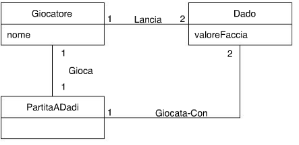
\includegraphics[scale=0.7]{images/Dadi.png}
\end{center}

\subsubsection{Assegnare responsabilità agli oggetti e 
disegnare diagrammi di interazione: \fancyglitter{responsabilità e collaborazioni}.}

\begin{center}
    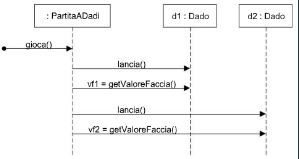
\includegraphics[scale = 0.7]{images/Dadi2.png}
\end{center}

\subsubsection{Definizione dei diagrammi delle classi di progetto.}

\begin{center}
    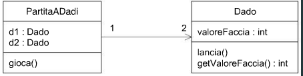
\includegraphics[scale=0.7]{images/Dadi 3.png}
\end{center}

}
\subsubsection{}
L'analisi dei requisiti e l'OOA/D vanno svolte nel contesto di un processo di sviluppo:

\begin{itemize}
    \item [$\Rightarrow$] Sviluppo iteratuivo;
    \item [$\Rightarrow$] Approccio agile;
    \item [$\Rightarrow$] Unified Process (UP).
\end{itemize}

\nt{ER e UML non sono pienamente adatti a possibili incrementi.}
\pagebreak

\subsection{UML}

\dfn{UML}{UML è un linguaggio \newfancyglitter{visuale} per la specifica,
la costruzione e la documentazione degli elaborati di un sistema software.

UML è uno standard per la notazione di diagrammi per disegnare o rappresentare
figure relative al software (specialmente OO).}
\subsubsection{}
UML è un \textit{abbozzo} o un \textit{progetto} per aiutare la comprensione nei team di sviluppo.
Il termine abbozzo indica che può essere soggetto a correzzione, ma se non ci 
sono feedback a tal proposito deve essere trattato come un dizionario.

\subsubsection{Uso di UML:}

\begin{itemize}
    \item [$\Rightarrow$] Punto di vista \fancyglitter{concettuale}: modello 
    di dominio, per visualizzare concetti del mondo reale;
    \item [$\Rightarrow$] Punto di vista \fancyglitter{software}: diagramma
    delle classi di progetto, utilizzata per visualizzare elementi software.
\end{itemize}

\subsubsection{Brevi note storiche:}

\begin{itemize}
    \item [$\Rightarrow$] Anni '60 e '70: nascita dei linguaggi OO (Simula e Smalltalk);
    \item [$\Rightarrow$] 1988: Bertrand Meyer, "Object-Oriented Software";
    \item [$\Rightarrow$] 1991: Jim Rumbaugh, "Object-Oriented Modelling and Design" (OOA/D);
    \item [$\Rightarrow$] 1991, Grady Booch, "Object-Oriented Software Engineering" (OOA/D e Casi d'Uso);
    \item [$\Rightarrow$] 1994, Rumbaugh e Booch fanno le prime proposte di UML;
    \item [$\Rightarrow$] Rational Corporation fondata dai "tre amigos" (Jacobson, Booch e Rumbaugh);
    \item [$\Rightarrow$] 1997 UML 1;
    \item [$\Rightarrow$] 2004 UML 2 (usato attualmente).
\end{itemize}

\section{Unified Process}

\dfn{Unified Process}{
    Unified Process è un processo iterativo ed evolutivo (incrementale)
    per lo sviluppo del software per la costruzione di sistemi orientati agli oggetti.
    Le iterazioni iniziali sono guidate dal \newfancyglitter{rischio}, dal
    \newfancyglitter{cliente} e dall'\newfancyglitter{architettura}.
}

\qs{}{Cosa c'è in UP?}

\begin{itemize}
    \item [$\Rightarrow$] Un'organizzazione del piano di progetto
    per fasi sequenziali;
    \item [$\Rightarrow$] Indicazioni sulle attività da svolgere nell'ambito
    di discipline e sulle loro inter-relazioni;
    \item [$\Rightarrow$] Un insieme di ruoli predefiniti;
    \item [$\Rightarrow$] Un insieme di artefatti da produrre.
\end{itemize}

\subsubsection{Un progetto UP è organizzato in 4 fasi:}

\begin{itemize}
    \item [$\Rightarrow$] \fancyglitter{Ideazione} (inception): visione approssimativa, studio economico, portata, stime approssimative di costi e tempi. \textbf{\underline{Milestone}:} \newfancyglitter{Obiettivi};
    \item [$\Rightarrow$] \fancyglitter{Elaborazione} (elaboration): visione raffinata, è un'implementazione iterativa del nucleo dell'architettura, risoluzione dei rischi maggiori, identificazione della maggior parte dei requisiti e della portata, stime più realistiche sulle loro inter-relazioni. \textbf{\underline{Milestone}:} \newfancyglitter{Architetturale};  
    \item [$\Rightarrow$] \fancyglitter{Costruzione} (construction): implementazione iterativa degli elementi rimanenti, più facili e a rischio minore, preparazione al rilascio. \textbf{\underline{Milestone}:} \newfancyglitter{Capacità operazionale};
    \item [$\Rightarrow$] \fancyglitter{Transizione} (transition): beta test, rilascio. \textbf{\underline{Milestone}:} \newfancyglitter{Rilascio prodotto}.
\end{itemize}

\begin{center}
    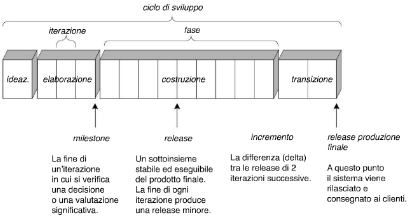
\includegraphics[scale = 1]{images/UP.png}
\end{center}

\wc{L'ideazione e l'elaborazione sono fasi di requisiti}{
    \begin{itemize}
        \item [$\Rightarrow$] L'Ideazione non è una fase di requisiti, ma di fattibilità;
        \item [$\Rightarrow$] L'Elaborazione non è una fase di requisiti o di progettazione, ma una fase in cui 
        si implementa in modo iterativo l'architettura del sistema e vengono ridotti i rischi maggiori.
    \end{itemize}
}

\subsection{Le discipline}

\dfn{Discipline}{
    Una disciplina è un insieme di attività e dei relativi \newfancyglitter{elaborati}
    in una determinata area, come le attività relative all'analisi dei requisiti. 
}

\cor{Elaborato}{
    Un elaborato (artefatto o work product) è il termine generico che indica un qualsiasi prodotto di lavoro: codice, schemi di basi di dati, 
    documenti di testo, diagrammi, modelli, etc.
}

\subsubsection{Discipline ingegneristiche di UP:}

\begin{itemize}
    \item [$\Rightarrow$] \fancyglitter{Modellazione del business}: attività che 
    modellano il dominio del problema e il suo ambito;
    \item [$\Rightarrow$] \fancyglitter{Requisiti}: attività di raccolra dei requisiti;
    \item [$\Rightarrow$] \fancyglitter{Progettazione} (analysis and design): attività di analisi dei requisiti
    e progetto architetturale;
    \item [$\Rightarrow$] \fancyglitter{Implementazione}: attività di progetto dettagliato e codifica del sistema, test sui componenti;
    \item [$\Rightarrow$] \fancyglitter{Test}: attività di controllo di qualità, test di integrazione e di sistema;
    \item [$\Rightarrow$] \fancyglitter{Rilascio}: attività di consegna e messa in opera.
\end{itemize}

\subsubsection{Discipline di supporto di UP:}

\begin{itemize}
    \item [$\Rightarrow$] \fancyglitter{Gestione delle configurazioni e del cambiamento}: attività di manutenzione durante il progetto;
    \item [$\Rightarrow$] \fancyglitter{Gestione progetto}: attività di pianificazione e governo del progetto;
    \item [$\Rightarrow$] \fancyglitter{Infrastruttura} (enviroment): attività che supportano il team di progetto, riguardo ai processi e strumenti utilizzati.
\end{itemize}

\nt{Nonostante le fasi siano \newfancyglitter{sequenziali}, le discipline non lo sono (perchè si eseguono in ogni iterazione).
Il numero di iterazioni dipende dal Project Manager.}

\subsubsection{Uso di UML in UP:}

\begin{itemize}
    \item [$\Rightarrow$] UP usa solo UML come linguaggio di modellazione;
    \item [$\Rightarrow$] I diagrammi UML si usano con variabilità, bisogna \newfancyglitter{personalizzare} UP;
    \item [$\Rightarrow$] I diagrammi si usano in UP seguendo le iterazioni e gli incrementi;
    \item [$\Rightarrow$] UP dice \newfancyglitter{quando} usare un diagramma;
    \item [$\Rightarrow$] In UP quasi tutto è \newfancyglitter{opzionale} eccetto che lo sviluppo iterativo e guidato dal rischio, la verifica continua della qualità e il codice;
    \item [$\Rightarrow$] La scelta delle pratiche e degli artefatti UP si riassume in un documento (\newfancyglitter{scenario di sviluppo}).
\end{itemize}

\subsection{Che cosa sono i requisiti?}

\dfn{Requisito}{
    Un requisito è una \newfancyglitter{capacità} o una condizione a cui il sistema deve essere \newfancyglitter{conforme}.
}

\cor{Sorgenti dei requisiti}{
    I requisiti derivano da richieste degli utenti del sistema per risolvere dei problemi e raggiungere degli obiettivi.
    Possono essere:
    \begin{itemize}
        \item [$\Rightarrow$] \fancyglitter{Requisiti funzionali}: descrivono il comportamento del sistema in termini di funzionalità offerte;
        \item [$\Rightarrow$] \fancyglitter{Requisiti non funzionali}: le proprietà del sistema nel suo complesso (sicurezza, prestazioni, etc.).
    \end{itemize}
}

\clm{}{}{
    In UP bisogna gestire i requisiti: si utilizza un approccio sistematico
    per trovare, documentare, organizza e tracciare i \underline{requisiti che cambiano}
    di un sistema. Si inizia a programmare quando sono stati specificati il 10\% o il 20\%
    dei requisiti significativi.
}

\subsubsection{Acquisizione sistematica dei requisiti:}

\begin{itemize}
    \item [$\Rightarrow$] Scrivere i Casi d'Uso con i clienti;
    \item [$\Rightarrow$] Workshop dei requisiti con sviluppatori e clienti;
    \item [$\Rightarrow$] Gruppi di lavoro con rappresentanti dei clienti;
    \item [$\Rightarrow$] Dimostrazione ai clienti dei risultati di ciascuna iterazione, per favorire un feedback.
\end{itemize}

\subsubsection{Modello FURPS+:}

\begin{itemize}
    \item [$\Rightarrow$] \fancyglitter{Funzionali} (F): requisiti funzionali e di sicurezza;
    \item [$\Rightarrow$] \fancyglitter{Usabilità} (U): facilità d'uso del sistema;
    \item [$\Rightarrow$] \fancyglitter{Affidabilità} (R - Reliability): disponibilità del sistema, capacità di tollerare guasti o di essere ripristinato;
    \item [$\Rightarrow$] \fancyglitter{Prestazioni} (P): tempi di risposta, throughput, capacità e uso delle risorse;
    \item [$\Rightarrow$] \fancyglitter{Sostenibilità} (S): facilità di modifica per riparazioni e miglioramenti, adattabilità, manutenibilità, localizzazione, configurazione, compatibilità;
    \item [$\Rightarrow$] \fancyglitter{+}: vincoli di progetto, interoperabilità, operazionali, fisici, legali, etc.
\end{itemize}

\subsubsection{Elaborati:}

\begin{itemize}
    \item [$\Rightarrow$] \fancyglitter{Modello dei Casi d'Uso}: scenari tipi dell'utilizzo di un sistema;
    \item [$\Rightarrow$] \fancyglitter{Specifiche supplementari}: ciò che non rientra nei Casi d'Uso, requisiti non funzionali o funzionali non esprimibili attraverso i Casi d'Uso;
    \item [$\Rightarrow$] \fancyglitter{Glossario}: termini significativi, dizionario dei dati;
    \item [$\Rightarrow$] \fancyglitter{Visione}: riassume i requisiti di alto livello, un documento sintetico per apprendere rapidamente le idee principali del progetto;
    \item [$\Rightarrow$] \fancyglitter{Regole di Business}: regole di dominio, i requisiti o le politiche che trascendono un unico progetto software e a cui un sistema deve conformarsi.
\end{itemize}

\section{Ideazione}

\qs{}{Che cos'è l'ideazione?}

\paragraph{Risposta:} l'ideazione permette di stabilire una visione completa
e la portata del progetto (\newfancyglitter{studio di fattibilità}).

\subsubsection{Durante l'ideazione:}

\begin{itemize}
    \item [$\Rightarrow$] Si analizzano il 10\% dei Casi d'Uso;
    \item [$\Rightarrow$] Si analizzano i requisiti non funzionali più importanti;
    \item [$\Rightarrow$] Si realizza una stima dei costi;
    \item [$\Rightarrow$] Si prepara l'ambiente di sviluppo;
    \item [$\Rightarrow$] \newfancyglitter{Durata:} breve.
\end{itemize}

\clm{}{}{Lo scopo dell'Ideazione \underline{non} è di raccogliere tutti i requisiti, né di generare
una stima o un piano di progetto affidabile.
Durante l'ideazione si cerca di capire se il progetto è fattibile e se ha senso.}

\definecolor{dkgreen}{rgb}{0, 0.5, 0}
\definecolor{mgray}{rgb}{0.9, 0.9, 0.9}
\begin{center}
    \begin{tabular}{ || >{\columncolor{mgray}}p{8cm} | >{\columncolor{GreenPastel}}p{8cm} ||}
    \hline\hline
        \rowcolor{lightgray}
    \textbf{Elaborato}& \textbf{\textcolor{dkgreen}{Commento}}\\ \hline
    \hline
        Visione e studio economico & Descrive obiettivi e vincoli di alto livello, fornisce un sommario del progetto.\\ \hline

        Modello dei Casi d'Uso & Descrive i requisiti funzionali del sistema. Vengono identificati i nomi della maggior parte dei Casi d'Uso.\\ \hline

        Specifiche supplementari & Descrive i requisiti non funzionali e i requisiti funzionali non esprimibili attraverso i Casi d'Uso.\\ \hline

        Glossario & Definisce i termini significativi del dominio.\\ \hline

        Lista dei Rischi e Piano di Gestione dei Rischi & Identifica i rischi principali e come affrontarli.\\ \hline

        Prototipi e proof of concept & Dimostrano la fattibilità tecnica e la comprensione dei requisiti.\\ \hline

        Piano dell'Iterazione & Fornisce una descrizione di cosa fare nella prima iterazione dell'elaborazione.\\ \hline

        Piano delle Fasi e Piano di Sviluppo del Software & Ipotesi (poco precise) riguardo la fase di elaborazione.\\ \hline 
    
        Scenario di Sviluppo & Descrive le pratiche e gli artefatti UP da usare.\\ \hline
    
        \hline

    \end{tabular}
\end{center}

\subsection{Artefatti nell'Ideazione}

\qs{}{La documentazione non è troppa?}

\paragraph{Risposta:} lo scopo della documentazione non è nel documento in sè, ma nel pensare:

\begin{itemize}
    \item [$\Rightarrow$] gli artefatti sono quelli che aggiungono valore;
    \item [$\Rightarrow$] sono parzialmente completati;
    \item [$\Rightarrow$] sono preliminari e approssimativi.
\end{itemize}

\nt{Nessun documento è definitivo.}

\dfn{Specifiche supplementari}{
    Le \newfancyglitter{specifiche supplementari} raccolgono altri requisiti,
    informazioni e vincoli che non sono espressi nei Casi d'Uso o nel Glossario. 
    Si deve mettere anche la cronologia delle versioni.
}

\subsection{Tipologie di documenti}

\dfn{Visione}{
    Il documento \newfancyglitter{Visione} riassume alcune informazioni contenute nel modello dei Casi d'Uso e 
    nelle Specifiche supplementari. Inoltre descrive brevemente il progetto ai partecipanti per stabilire una
    visione comune.
    
    \begin{itemize}
        \item [$\Rightarrow$] Obiettivi e problemi fondamentali ad alto livello\footnote{Soprattutto per i requisiti non funzionali};
        \item [$\Rightarrow$] Riepilogo delle caratteristiche di sistema.
    \end{itemize}
}

\nt{Spesso è utile iniziare da un Glossario.}

\dfn{Glossario e dizionario dei dati}{
    Il \newfancyglitter{Glossario} è un documento che definisce i termini significativi del dominio e le relazioni tra di
    essi. Si devono eliminare eventuali discrepanze per ridurre problemi di comunicazione e di ambiguità.

    In UP il Glossario svolge anche il ruolo di \newfancyglitter{dizionario dei dati}:
    un documento di dati che si riferiscono ad altri dati\footnote{Metadati.}, per esempio le regole di validazione.
}

\cor{Regole di dominio}{
    Le \newfancyglitter{regole di dominio} (o regole di Business\footnote{Viste in "Basi di dati".}) stabiliscono
    come può funzionare un dominio o un business.

}


\section{Casi d'Uso}

\subsection{Disciplina dei requisiti}

\dfn{Disciplina dei requisiti}{
    La \newfancyglitter{disciplina dei requisiti} è il processo
    per scoprire cosa deve essere costruito e orientare lo sviluppo verso 
    il sistema corretto.
}

\cor{Requisiti di sistema}{
    I requisiti di sistema sono le capacità e le condizioni
    a cui il sistema deve essere conforme.
}

\nt{I requisiti di sistema sono scritti nel "linguaggio del cliente".}

\subsubsection{Passi principali:}

\begin{itemize}
    \item [$\Rightarrow$] Produrre una \fancyglitter{lista dei requisiti potenziali} (candidati);
    \item [$\Rightarrow$] Capire il \fancyglitter{contesto} del sistema;
    \item [$\Rightarrow$] Catturare i \fancyglitter{requisiti funzionali} (di comportamento);
    \item [$\Rightarrow$] Catturare i \fancyglitter{requisiti non funzionali}.
\end{itemize}

\subsubsection{Ogni requisito è caratterizzato da:}

\begin{itemize}
    \item [$\Rightarrow$] \fancyglitter{Breve descrizione};
    \item [$\Rightarrow$] \fancyglitter{Stato} (proposto, approvato, incorporato, validato);
    \item [$\Rightarrow$] \fancyglitter{Costi di implementazione stimati};
    \item [$\Rightarrow$] \fancyglitter{Priorità};
    \item [$\Rightarrow$] \fancyglitter{Rischio associato per la sua implementazione}.
\end{itemize}

\dfn{Lista dei requisiti}{
    La \newfancyglitter{lista dei requisiti} è usata per stimare la taglia del progetto e per
    decidere come suddividere il lavoro in sequenze di iterazioni.
}

\subsection{Capire il contesto del sistema e catturare i requisiti}

\subsubsection{Ci sono due modi per capire il contesto del sistema:}

\begin{itemize}
    \item [$\Rightarrow$] \fancyglitter{Modello di dominio}: descrive i concetti significativi del sistema come oggetti del dominio e relaziona i concetti con associazioni (usa UML);
    \item [$\Rightarrow$] \fancyglitter{Modello di business}: un super-insieme del modello di dominio, descrive i processi di business. È un prodotto dell'ingegneria del business e ha lo scopo di migliorare i processi di business. 
\end{itemize}

\nt{Il contesto del sistema è catturato dal \newfancyglitter{diagramma UML dei Casi d'Uso}.}

\subsubsection{Catturare i requisiti funzionali:}

\begin{itemize}
    \item [$\Rightarrow$] In UP vengono usati i Casi d'Uso;
    \item [$\Rightarrow$] Un Caso d'Uso rappresenta un possibile utilizzo del sistema da parte di un utente;
    \item [$\Rightarrow$] Sono descrizioni testuali.
\end{itemize}

\subsubsection{Catturare i requisiti non funzionali:}

\begin{itemize}
    \item [$\Rightarrow$] Si utilizzano le Specifiche supplementari;
    \item [$\Rightarrow$] Possono ancge essere catturati nei Casi d'Uso.
\end{itemize}

\subsection{Casi d'Uso e UP}

\subsubsection{UP è una metodologia "\fancyglitter{use-case driven}":}
\begin{itemize}
    \item [$\Rightarrow$] I Casi d'Uso si usano per pianificare le iterazioni;
    \item [$\Rightarrow$] L'analisi e la progettazione si basano sui Casi d'Uso;
    \item [$\Rightarrow$] I Casi d'Uso sono usati per definire i test;
    \item [$\Rightarrow$] I Casi d'Uso influiscono nella redazione dei manuali utente e della Visione;
    \item [$\Rightarrow$] \fancyglitter{Attori}: qualcosa o qualcuno dotato di \newfancyglitter{comportamento};
    \item [$\Rightarrow$] \fancyglitter{Scenario} (istanza di Caso d'Uso): \newfancyglitter{sequenza specifica di azioni e interazioni} tra l sistema e alcuni attori. Descrive una particolare storia;
    \item [$\Rightarrow$] \fancyglitter{Caso d'Uso}: \newfancyglitter{insieme di scenari} che descrivono un attore che usa il sistema per \newfancyglitter{raggiungere un obiettivo specifico}.
\end{itemize}

\nt{I Casi d'Uso possono essere di successo o di fallimento.}

\wc{I Casi d'Uso sono diagrammi}{
    I Casi d'Uso sono sono documenti di testo, non diagrammi.
}
\pagebreak
\ex{Caso d'Uso: breve descrizione}{
    \begin{center}
        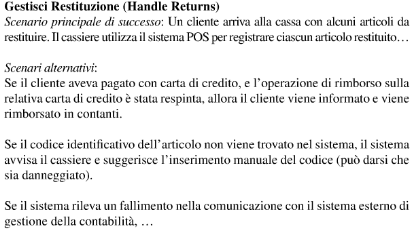
\includegraphics[scale = 0.7]{images/Gestisci restituzione.png}
    \end{center}

}

\dfn{Modello dei Casi d'Uso}{
    Il \newfancyglitter{modello dei Casi d'Uso} è un modello delle funzionalità del sistema. Include un diagramma
    UML dei Casi d'Uso che funge da \newfancyglitter{modello di contesto} del sistema e da \newfancyglitter{indice dei nomi} di Caso d'Uso.

}

\nt{I Casi d'Uso sono utili per rappresentare i requisiti come OOA/D.

I Casi d'Uso definiscono i \newfancyglitter{contratti} (vedi sezione \ref{contratti}) in relazione al comportamento del sistema.}


\subsubsection{L'enfasi è posta sull'utente:}
\begin{itemize}
    \item [$\Rightarrow$] Chi utilizza il sistema?
    \item [$\Rightarrow$] Quali sono i loro Scenari d'Uso tipici?
    \item [$\Rightarrow$] Quali sono i loro obiettivi?
    \item [$\Rightarrow$] \underline{Non} sono caratteristiche del sistema (il "come" si vedrà nella progettazione).
\end{itemize}

\subsection{Attori e tipi di attori}

\dfn{Attore}{
    Un \newfancyglitter{attore} è qualcosa o qualcuno dotato di comportamento.
}

\nt{Il sistema stesso è considerato un attore.}

\subsubsection{Gli attori sono \fancyglitter{ruoli} svolti da persone, organizzazioni, software e macchine:}

\begin{itemize}
    \item [$\Rightarrow$] \fancyglitter{Attore primario}:
    \begin{itemize}
        \item Raggiunge gli obiettivi utente utilizzando il sistema;
        \item Utile per trovare gli obiettivi utente.
    \end{itemize}
    \item [$\Rightarrow$] \fancyglitter{Attore di supporto}:
    \begin{itemize}
        \item Offre un servizio al sistema;
        \item Utile per chiarire le interfacce esterne e i protocolli.
    \end{itemize}
    \item [$\Rightarrow$] \fancyglitter{Fuori scena}:
    \begin{itemize}
        \item Ha un interesse nel comportamento del Caso d'Uso;
        \item Utile per garantire che tutti gli interessi necessari vengano soddisfatti.
    \end{itemize}
\end{itemize}

\subsection{Formato di un Caso d'Uso}

\subsubsection{Un Caso d'Uso può avere tre formati distinti:}

\begin{itemize}
    \item [$\Rightarrow$] \fancyglitter{Breve}: un paragrafo, relativo allo scenario principale di successo. Serve a capire rapidamente l'\newfancyglitter{argomento} e la \newfancyglitter{portata};
    \item [$\Rightarrow$] \fancyglitter{Informale}: più paragrafi, scritti in modo informale, relativi a vari scenari. Si ha un maggior livello di dettaglio;
    \item [$\Rightarrow$] \fancyglitter{Dettagliato}: tutti i passi e le variazioni sono scritti in dettaglio, include \newfancyglitter{pre-condizioni} e \newfancyglitter{garanzie di successo}. Si scrivono a partire da un formato breve o informale.
\end{itemize}

\nt{Durante l'Ideazione il 10\% dei Casi d'Uso è riportato
in formato dettagliato utilizzando appositi \newfancyglitter{template}}

\begin{center}
    \begin{tabular}{ || >{\columncolor{mgray}}p{8cm} | >{\columncolor{GreenPastel}}p{8cm} ||}
    \hline\hline
        \rowcolor{lightgray}
    \textbf{Sezione del Caso d'Uso}& \textbf{\textcolor{dkgreen}{Commento}}\\ \hline
    \hline
        Nome del Caso d'Uso & Inizia con un verbo. \\\hline

        Portata & Il sistema che si sta progettando. \\\hline

        Livello & "Obiettivo utente" o "sottofunzione". \\\hline

        Attore primario & Usa direttamente il sistema; gli chiede
        di fornire i suoi servizi per raggiungere un obiettivo. \\\hline

        Parti interessate e interessi & Chiunque abbia un interesse nel comportamento del Caso d'Uso e che cosa desidera. \\\hline

        Pre-condizioni & Stato del sistema prima che il Caso d'Uso inizi. Ciò che vale la pena di dire al lettore. \\\hline

        Garanzia di successo & Che cosa deve essere vero se il Caso d'Uso viene completato con successo. Ciò che vale la pena di dire al lettore. \\\hline  

        Scenario principale di successo & Uno scenario comune di attraversamento del Caso d'Uso, di successo e incondizionato. \\\hline

        Estensioni & Scenari alternativi, di successo o di fallimento. \\\hline

        Requisiti speciali & Requisiti non funzionali correlati. \\\hline

        Elenco delle varianti tecnologiche e dei dati & Varianti dei metodi di I/O e nel formato dei dati. \\\hline

        Frequenza di ripetizione & Quanto spesso si prevede che il Caso d'Uso venga eseguito. \\\hline

        Varie & Altri aspetti. \\\hline

        \hline

    \end{tabular}
\end{center}


\subsection{Come scrivere un Caso d'Uso}

\subsubsection{Sezioni del Caso d'Uso:}

\begin{itemize}
    \item [$\Rightarrow$] \fancyglitter{Portata}: descrive i confini del sistema;
    \item [$\Rightarrow$] \fancyglitter{Livello}: "obiettivo utente" o "sottofunzione";
    \item [$\Rightarrow$] \fancyglitter{Attore finale, attore primario}: l'attore
    finale è l'attore che vuole raggiungere un obiettivo e questo richiede l'esecuzione dei servizi
    del sistema. L'attore primario è l'attore che usa direttamente il sistema. Spesso coincidono;
    \item [$\Rightarrow$] \fancyglitter{Parti interessate}: chiunque abbia un interesse nel comportamento del Caso d'Uso;
    \item [$\Rightarrow$] \fancyglitter{Pre-condizioni}: lo stato del sistema prima che il Caso d'Uso inizi. Non vengono verificate all'interno del Caso d'Uso;
    \item [$\Rightarrow$] \fancyglitter{Garanzie di successo} (post-condizioni): ciò che deve essere vero se il Caso d'Uso viene completato con successo.
\end{itemize}

\subsubsection{Caratteristiche:}

\begin{itemize}
    \item [$\Rightarrow$] Lo scenario principale viene anche chiamato "\fancyglitter{percorso felice}", "flusso
    di base" o "flusso tipico";
    \item [$\Rightarrow$] Lo scenario principale è costituito da una sequenza di passi, che può contenere passi da ripetere, ma che non comprende nessuna diramazione\footnote{\underline{Non} è un algoritmo.};
    \item [$\Rightarrow$] La gestione del comportamento condizionale e delle alternative viene descritta nelle "\fancyglitter{estensioni}".
\end{itemize}

\subsubsection{I passi possono essere di 3 tipi:}

\begin{itemize}
    \item [$\Rightarrow$] \fancyglitter{Un'interazione tra attori}: 
    \begin{itemize}
        \item Un attore chiede qualcosa al sistema o inserisce dei dati;
        \item Il sistema interagisce con l'attore, rispondendo o comunicando dei dati;
        \item Il sistema interagisce con altri sistemi.
    \end{itemize}
    \item [$\Rightarrow$] \fancyglitter{Un cambiamento di stato da parte del sistema};
    \item [$\Rightarrow$] \fancyglitter{Una validazione}: normalmente fatta dal sistema.
\end{itemize}

\nt{Il primo passo indica l'evento \textit{trigger} che scatena l'esecuzione dello scenario.}

\subsubsection{Estensioni:}

\begin{itemize}
    \item [$\Rightarrow$] Descrivono tutti gli altri scenari;
    \item [$\Rightarrow$] Sono descritte per differenza rispetto allo scenario principale;
    \item [$\Rightarrow$] Vengono indicate con riferimento a un passo dello scenario principale;
    \item [$\Rightarrow$] Sono composte da:
    \begin{itemize}
        \item \fancyglitter{Condizione}: che scatena l'estensione;
        \item \fancyglitter{Gestione}: come viene gestita l'estensione. Può essere di un unico passo o di più passi.
    \end{itemize}
\end{itemize}

\nt{Le condizioni vanno scritte, se possibile, come qualcosa che può essere rilevato da un attore.}

\cor{Utilizzo delle estensioni}{
    \begin{itemize}
        \item [$\Rightarrow$] L'attore vuole che l'esecuzione principale del Caso d'Uso proceda in modo diverso da quanto previsto nel percorso felice;
        \item [$\Rightarrow$] Il Caso d'Uso deve procedere diversamente da quanto previsto ed è il sistema che se ne accorge (durante un'azione o una validazione);
        \item [$\Rightarrow$] Un passo dello scenario principale descrive un'azione generica o astratta, mentre le estensioni
        descrivono azioni specifiche o concrete.
    \end{itemize}
}
\pagebreak
\subsubsection{Notazione:}

\begin{itemize}
    \item [$\Rightarrow$] Si può utilizzare il formato a due colonne. Questo enfatizza
    la \fancyglitter{conversazione} tra gli attori e il sistema\footnote{È il formato scelto per il laboratorio del corso.}.
    \begin{figure}[!h]
        \centering
        \subfloat[Rappresentazione come conversazione]{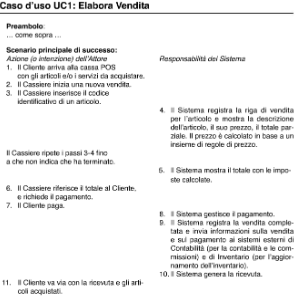
\includegraphics[scale = 0.65]{images/Notazione.png}} 
        \subfloat[Relativa tabella]{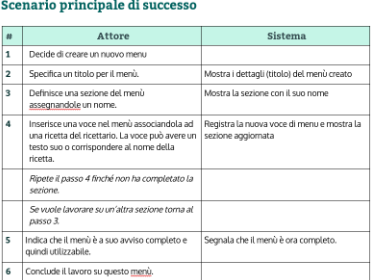
\includegraphics[scale = 0.65]{images/Notazione2.png}}
    \end{figure}
    \item [$\Rightarrow$] Le estensioni vanno indicate con riferimento al passo dello scenario principale.
\begin{figure}[!h]
    \centering
    \subfloat[Estensione del punto 1]{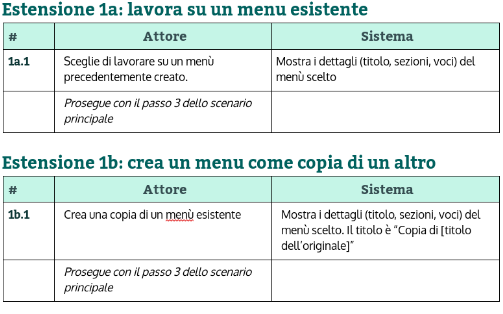
\includegraphics[scale = 0.4]{images/Estensione1.png}} 
    \subfloat[Estensione del punto 3]{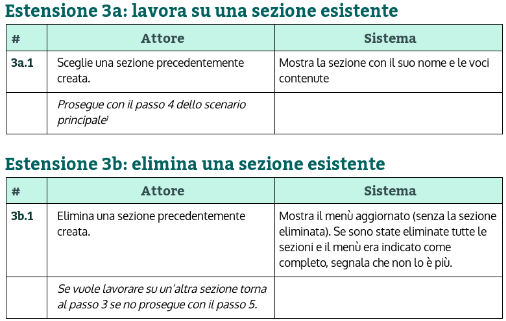
\includegraphics[scale = 0.4]{images/Estensione2.png}}
\end{figure}
\item [$\Rightarrow$] Ci possono essere alternative che possono occorrere in più passi.
\begin{figure}[!h]
    \centering
    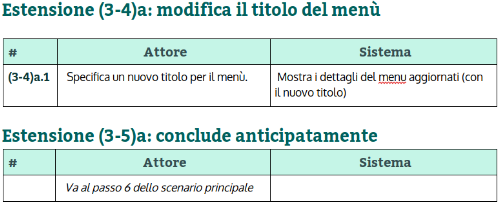
\includegraphics[scale = 0.55]{images/Estensione3.png}
\end{figure}
\end{itemize}

\ex{Passi ed estensioni}{
    \begin{center}
        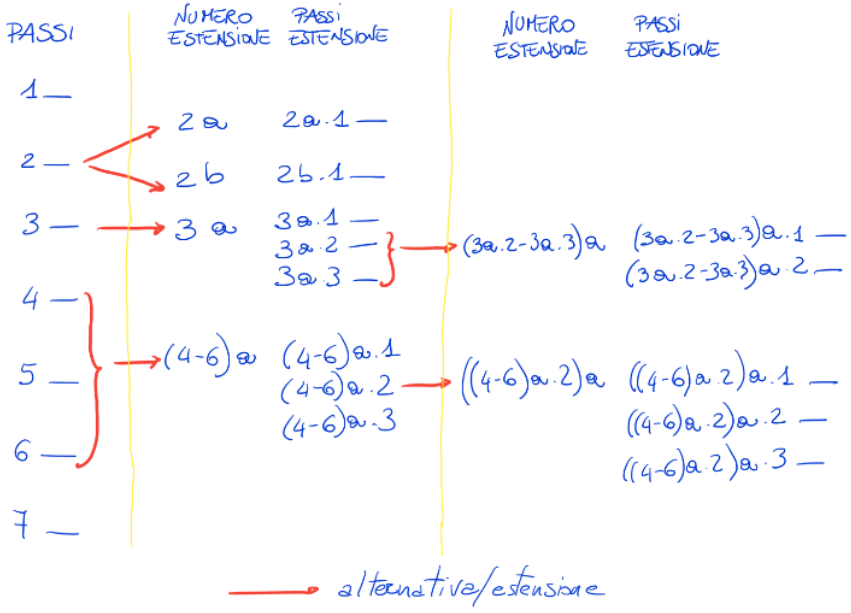
\includegraphics[scale = 0.4]{images/Passi ed estensioni.png}
    \end{center}
}

\nt{Lo stile deve essere \newfancyglitter{essenziale} e \newfancyglitter{coinciso}. Si ignora l'interfaccia utente, ci si concentra sull'Obiettivo Utente.}

\dfn{Stile essenziale}{
    La narrativa è espressa a livello di \newfancyglitter{intenzioni} e 
    \newfancyglitter{responsabilità}, non con riferimento ad azioni concrete.
    Le intenzioni e le responsabilità devono rimanere indipendenti dai dettagli tecnologici e dagli attori.
}

\ex{Stile}{
    \begin{itemize}
        \item [\textcolor{dkgreen}{\checkmark}] L'Amministratore si identifica.
        \item [\textcolor{dkgreen}{\checkmark}] Il Sistema autentica l'identità.
        \item [\textcolor{red}{\XSolidBrush}] L'Amministratore inserisce ID e password nella finestra di dialogo.
        \item [\textcolor{red}{\XSolidBrush}] Il sistema autentica l'Amministratore.
        \item [\textcolor{red}{\XSolidBrush}] Il sistema visualizza la finestra "edit users".
    \end{itemize}
}

\clm{}{}{Durante l'analisi dei requisiti bisogna specificare il comportamento
esterno del Sistema, considerato a "scatola nera". Non bisogna prendere decisioni
sul "come".

\begin{itemize}
    \item [\textcolor{red}{\XSolidBrush}] Il Sistema memorizza la vendita in una base di dati.
    \item [\textcolor{red}{\XSolidBrush}] Il Sistema esegue un'istruzione SQL INSERT per la vendita.
\end{itemize}
}

\subsection{Trovare i Casi d'Uso}

\begin{enumerate}
    \item Scegliere i confini del Sistema;
    \item Identificare gli attori primari;
    \item Identificare gli obiettivi di ciascun attore primario;
    \item Definire i Casi d'Uso che soddisfano gli obiettivi degli utenti.
\end{enumerate}

\ex{Identificare gli attori primari}{
    \begin{center}
        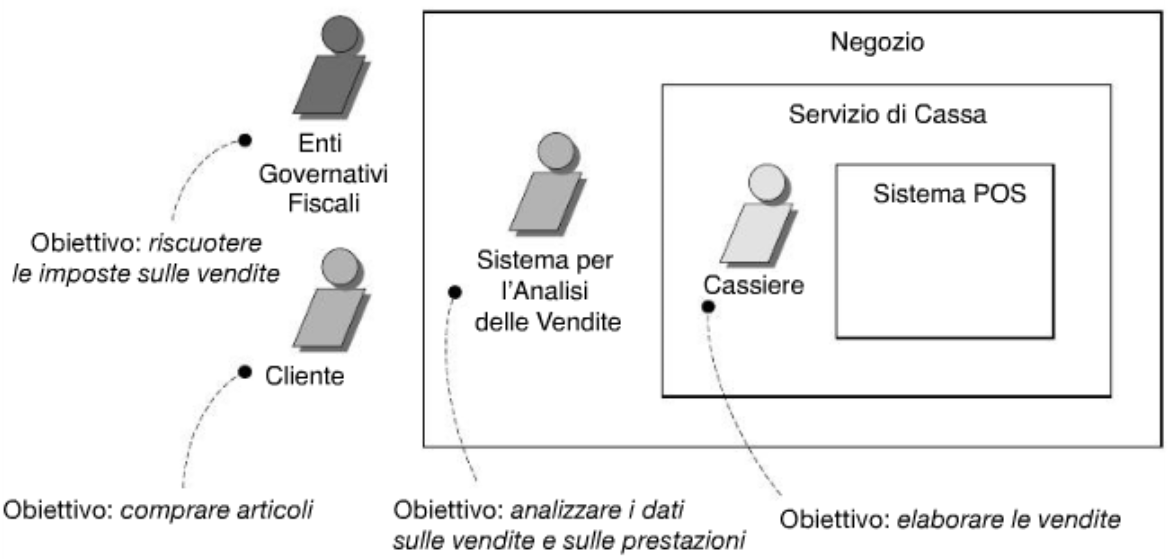
\includegraphics[scale = 0.3]{images/Identificare gli attori primari.png}
        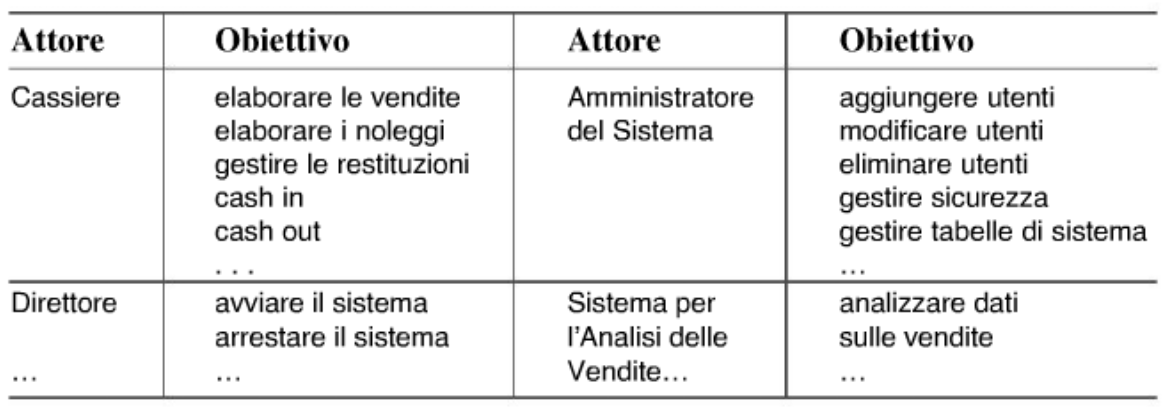
\includegraphics[scale = 0.3]{images/Identificare gli attori 2.png}
    \end{center}

}

\qs{}{Qual è un livello utile per esprimere i Casi d'Uso nell'analisi dei requisiti di un'applicazione software?}
\begin{itemize}
    \item [$\Rightarrow$] Il test del \fancyglitter{capo}: il capo sarà felice?
    \item [$\Rightarrow$] Il test \fancyglitter{EBP} (Elementary Business Process): un processo di Business è un'attività che aggiunge un valore;
    \item [$\Rightarrow$] Il test della \fancyglitter{dimensione}: un Caso d'Uso raramente richiede una singola azione o passo. Normalmente, nella forma dettagliata, richiede dalle 3 alle 10 pagine.
\end{itemize}

\ex{Verificare l'utilità dei Casi d'Uso}{
    \begin{itemize}
        \item \textcolor{red}{\XSolidBrush} Negoziare un contratto con un fornitore.
        \begin{itemize}
            \item [$\Rightarrow$] Troppo grande.

        \end{itemize}
        \item \textcolor{dkgreen}{\checkmark} Gestire una restituzione.
        \begin{itemize}
            \item [$\Rightarrow$] D'accordo con il capo, simile a EBP, dimensioni adeguate.
        \end{itemize}
        \item \textcolor{red}{\XSolidBrush} Effetture il login.
        \begin{itemize}
            \item [$\Rightarrow$] Il capo non è contento se ci si limita a fare solo quello tutta la giornata.
        \end{itemize}
        \item \textcolor{red}{\XSolidBrush} Spostare una pedina sul tabellone da gioco.
        \begin{itemize}
            \item [$\Rightarrow$] Passo singolo, non supera il test della dimensione.
        \end{itemize}
    \end{itemize}
}

\subsection{Livello dei Casi d'Uso}

\dfn{Livello di obiettivo utente}{
    Nell'analisi dei requisiti è utile concentrarsi sui casi utente EBP.
}

\dfn{Livello di sotto-funzione}{
    Rappresenta una funzionalità nell'uso del sistema.
    Utile per mettere a fattor comune sequenze di passi condivise da più Casi
    d'Uso, evitando duplicazione di testo.
}

\ex{Diagramma dei Casi d'Uso (UCD)}{
    \begin{center}
        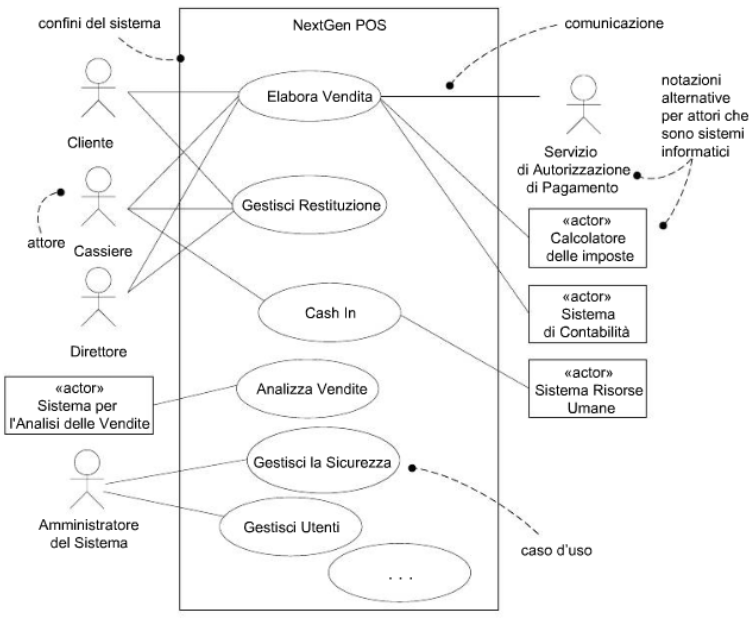
\includegraphics[scale = 0.5]{images/UCD.png}
    \end{center}

}
\section{Elaborazione}

\dfn{Elaborazione}{
    L'elaborazione è la serie iniziale di iterazioni durante le quali il team
    esegue un'indagine seria, implementa il nucleo dell'architettura,
    chiarisce la maggior parte dei requisiti e affronta le problematiche
    più rischiose.
}

\nt{Durante questa fase vengono creati prototipi "usa e getta" ma codice
e progettazione sono parti di qualità-produzione del sistema finale.}

\subsection{Pianificazione dell'iterazione successiva}

I requisiti e le iterazioni sono organizzate in base a:

\begin{itemize}
    \item [$\Rightarrow$] \fancyglitter{Rischio}: tecnico, incertezza dello sforzo, usabilità;
    \item [$\Rightarrow$] \fancyglitter{Copertura}: le iterazioni iniziali devono coprire tutte le parti principali del sistema;
    \item [$\Rightarrow$] \fancyglitter{Criticità}: le funzioni che il cliente ritiene più importanti.
\end{itemize}

\clm{}{}{La classifica viene stilata prima dell'iterazione 1, poi prima dell'iterazione 2 e così via. La lista non è definitiva.

\begin{center}
    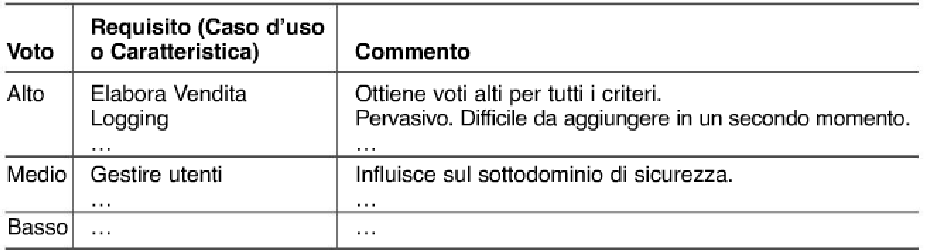
\includegraphics[scale=0.48]{images/Classifica.png}
\end{center}
}

\dfn{Iterazione 1}{
    Nell'iterazione 1 si implementa un sottoinsieme dei requisiti o dei Casi d'Uso completi.
}

\subsection{Artefatti dell'Elaborazione}

\begin{center}
    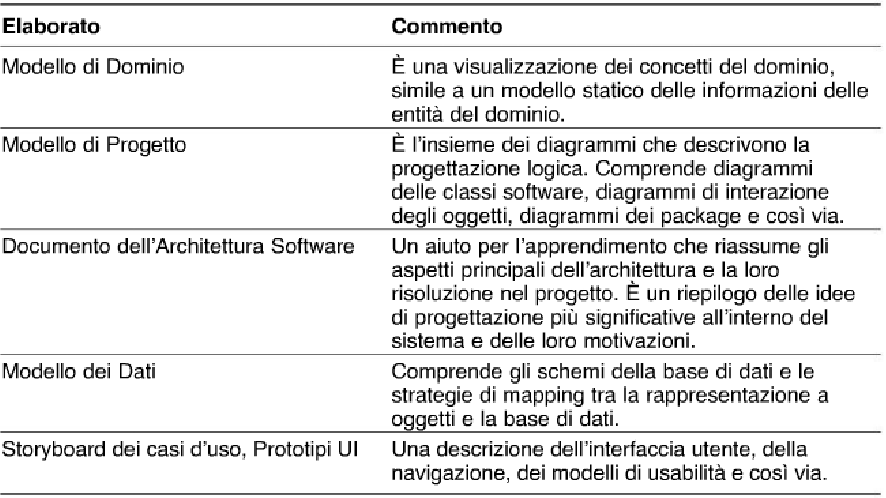
\includegraphics[scale=0.5]{images/Artefatti elaborazione.png}
\end{center}

\begin{center}
    
\end{center}

\section{Modello di Dominio}

\dfn{Modello di Dominio}{
    Il \newfancyglitter{Modello di Dominio} è una rappresentazione visuale
    delle classi concettuali (oggetti del dominio). Include:
    \begin{itemize}
        \item [\textcolor{green}{\checkmark}] \newfancyglitter{Oggetti} di dominio.
        \item [\textcolor{green}{\checkmark}] \newfancyglitter{Associazioni} tra classi concettuali.
        \item [\textcolor{green}{\checkmark}] \newfancyglitter{Attributi} di classi concettuali.
        \item [\textcolor{red}{\XSolidBrush}] \newfancyglitter{Operazioni}.
    \end{itemize}
}

\nt{Non è un modello di dati.}

\ex{Modello di dominio}{
    \begin{center}
        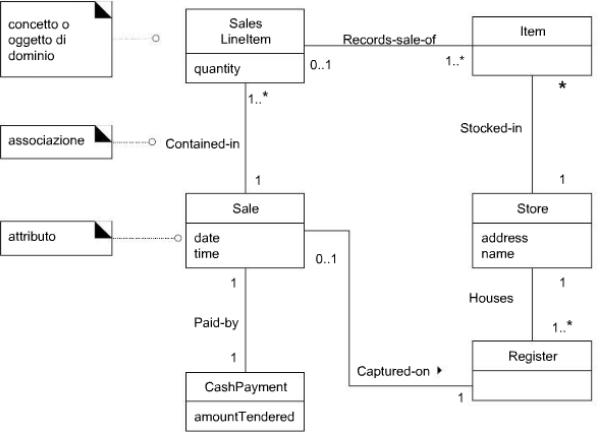
\includegraphics[scale=0.5]{images/Modello di dominio.png}
    \end{center}

}

\subsection{Classi concettuali}

\dfn{Classi concettuali}{
    Una \newfancyglitter{classe concettuale} rappresenta un concetto
    del mondo reale o del dominio di interesse di un sistema che si sta modellando.

    \begin{itemize}
        \item [$\Rightarrow$] Il \newfancyglitter{simbolo} è una parola 
        o un'immagine usata per rappresentare la classe concettuale;
        \item [$\Rightarrow$] L'\newfancyglitter{intensione} è la definizione della classe concettuale;
        \item [$\Rightarrow$] L'\newfancyglitter{estensione} è l'insieme di oggetti che la classe concettuale rappresenta.
    \end{itemize}
}
\pagebreak
\cor{Associazioni}{
    Un'associazione è una relazione tra istanze di classi
    che indica una connessione significativa e interessante.
}

\ex{Associazione}{
    \begin{center}
        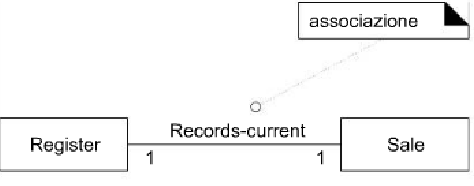
\includegraphics[scale=0.5]{images/Associazione.png}
    \end{center}


}

\cor{Attributi}{
    Un attributo è un valore logico degli oggetti di una classe.
}

\ex{Attributo}{
    \begin{center}
        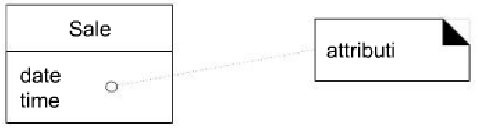
\includegraphics[scale=0.5]{images/Attributo.png}
    \end{center}
}

\subsubsection{Riduzione del "gap di rappresentazione":}

\begin{itemize}
    \item [$\Rightarrow$] \fancyglitter{Comprendere} il dominio del sistema da realizzare e il suo vocabolario;
    \item [$\Rightarrow$] \fancyglitter{Definire} un \fancyglitter{linguaggio comune} che abiliti la comunicazione tra le diverse parti;
    \item [$\Rightarrow$] Come \fancyglitter{fonte di ispirazione} per la progettazione dello strato di dominio.
\end{itemize}

\qs{}{Come creare un Modello di Dominio}

\begin{itemize}
    \item [$\Rightarrow$] Trovare le classi concettuali;
    \item [$\Rightarrow$] Disegnarle come classi in UML;
    \item [$\Rightarrow$] Aggiungere le associazioni;
    \item [$\Rightarrow$] Aggiungere gli attributi.
\end{itemize}

\subsection{Trovare le classi concettuali}

\begin{itemize}
    \item [$\Rightarrow$] Riuso-modifica di modelli esistenti (pattern);
    \item [$\Rightarrow$] Utilizzo di elenchi di categorie;
    \item [$\Rightarrow$] Analisi linguistica delle descrizioni testuali di un dominio. 
    Si utilizano i Casi d'Uso dettagliati.
\end{itemize}

\dfn{Classi Descrizione}{
    Una \newfancyglitter{classe descrizione} contiene informazioni
    che descrivono qualcos'altro. È utile avere un'associazione
    che collega la classe descrizione alla classe descritta\footnote{Pattern Item-Descriptor.}.
}

\ex{Classe descrizione}{
    \begin{center}
        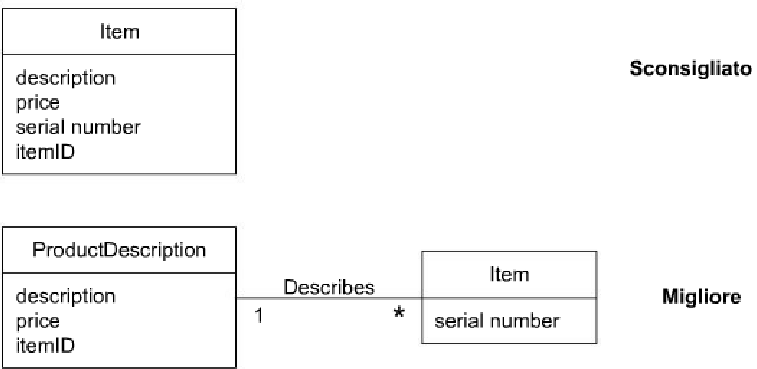
\includegraphics[scale=0.5]{images/Classe descrizione.png}
    \end{center}
}

\subsection{Associazioni}

\subsubsection{È utile includere:}

\begin{itemize}
    \item [$\Rightarrow$] Associazioni la cui conoscenza della relazione deve
    essere mantenuta dal sistema;
    \item [$\Rightarrow$] Associazioni derivate dall'elenco di associazioni comuni.
\end{itemize}

\nt{Un'associazione è per natura \fancyglitter{bidirezionale}.}

\begin{center}
    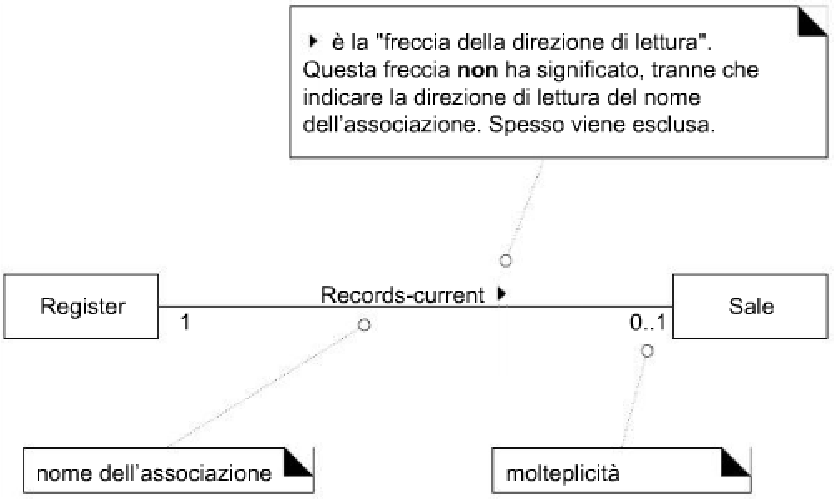
\includegraphics[scale=0.4]{images/Associazione2.png}
\end{center}

\subsubsection{Caratteristiche delle associazioni:}

\begin{itemize}
    \item [$\Rightarrow$] \fancyglitter{Nome significativo}: NomeClasse-FraseVerbale-NomeClasse;
    \item [$\Rightarrow$] \fancyglitter{Molteplicità e direzione di lettura}.
\end{itemize}

\dfn{Ruoli}{
    Un \newfancyglitter{ruolo} è l'estremità di un'associazione. I ruoli possono avere:
    \begin{itemize}
        \item [$\Rightarrow$] \newfancyglitter{Nome};
        \item [$\Rightarrow$] \newfancyglitter{Molteplicità};
        \item [$\Rightarrow$] \newfancyglitter{Navigabilità}.
    \end{itemize}


}

\cor{Molteplicità}{
    La molteplicità di un ruolo definisce quante istanze di una classe possono
    essere associate a un'istanza dell'altra classe.
}

\ex{Molteplicità}{
    \begin{center}
        \includegraphics[scale=0.5]{images/Molteplicità.png}
    \end{center}
}

\subsection{Composizione}

\dfn{Composizione}{
    La \newfancyglitter{composizione}, o aggregazione composta,
    è un tipo forte di aggregazione intero-parte:
    \begin{itemize}
        \item [$\Rightarrow$] Ciascuna istanza della parte appartiene a una sola istanza del composto alla volta;
        \item [$\Rightarrow$] La parte non può esistere senza il composto;
        \item [$\Rightarrow$] La vita delle parti è limitata a quella del composto.
    \end{itemize}
}

\subsection{Attributi}

\subsubsection{Caratteristiche degli attributi:}

\begin{itemize}
    \item [$\Rightarrow$] \fancyglitter{Origine}: derivati/non derivati;
    \item [$\Rightarrow$] \fancyglitter{Tipo di dato}: vincolo sui valori del dominio.
\end{itemize}

\begin{center}
    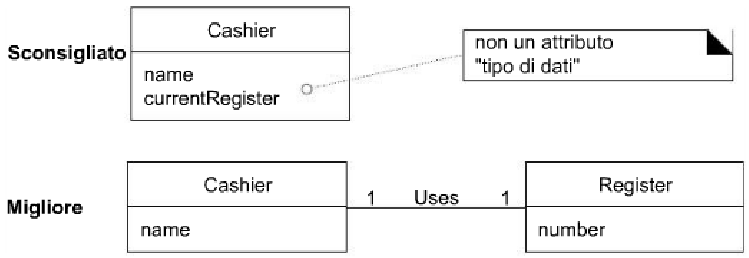
\includegraphics[scale=0.5]{images/Attributi2.png}
\end{center}

\nt{Se non si pensa a un concetto come a un numero, un testo o un
valore allora probabilmente è una classe, non un attributo.}

\begin{center}
    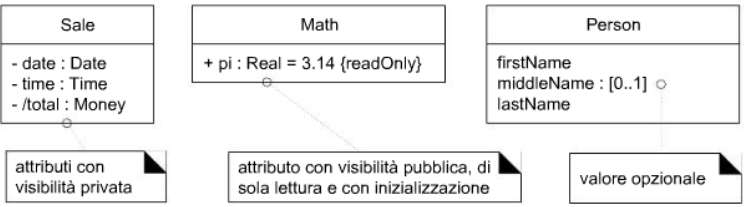
\includegraphics[scale=0.5]{images/Notazione attributi.png}
\end{center}


\subsection{Verifiche del modello}

\begin{itemize}
    \item [$\Rightarrow$] Verificare le classi concettuali introdotte:
    \begin{itemize}
        \item Alternativa classe classe-attributo attributo;
        \item Classi descrizione.
    \end{itemize}
    \item [$\Rightarrow$] Verificare le associazioni:
    \begin{itemize}
        \item Indipendenza delle associazioni diverse relative alle stesse classi.
    \end{itemize}
    \item [$\Rightarrow$] Verificare gli attributi:
    \begin{itemize}
        \item Non intrododurre attributi per riferirsi ad altre classi (chiavi esterne).
    \end{itemize}
\end{itemize}

\ex{Modello di Dominio (parziale)}{
    \begin{center}
        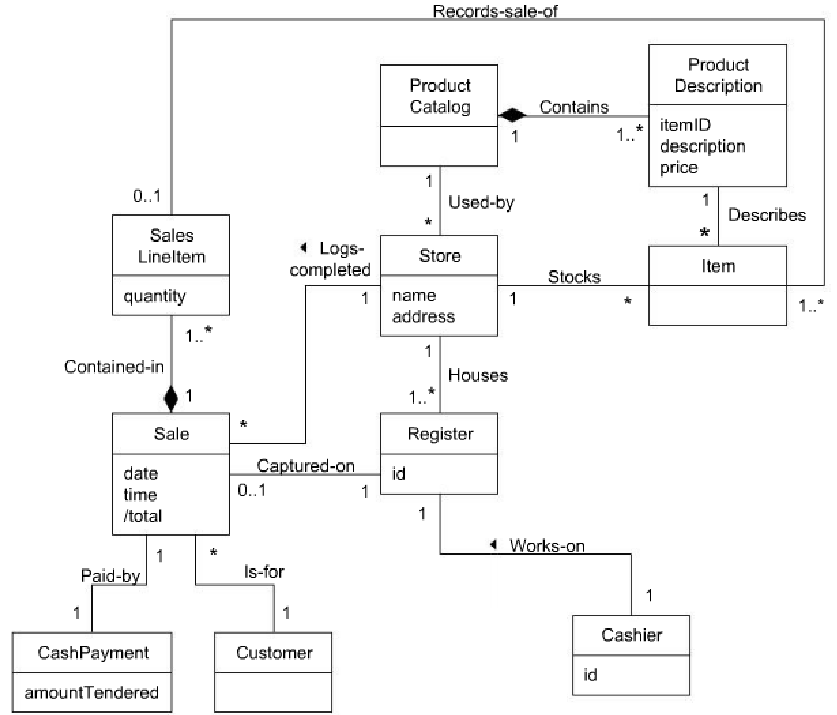
\includegraphics[scale=0.5]{images/Modello di Dominio.png}
    \end{center}

}
\dfn{Generalizzazione}{
    La \newfancyglitter{generalizzazione} è un'astrazione basata sull'identificazione
    di caratteristiche comuni tra concetti, che porta a definire un concetto più generale 
    (superclasse) e concetti più specifici (sottoclassi). Vale il principio di sostituibilità.
}

\ex{Generalizzazione}{
    \begin{center}
        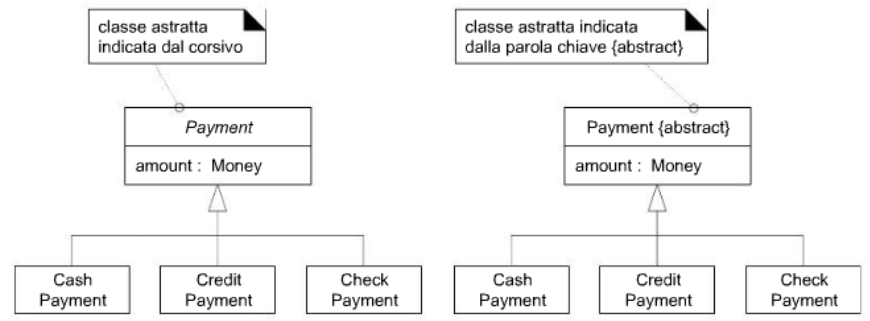
\includegraphics[scale=0.45]{images/Generalizzazione.png}
    \end{center}


}

\section{Diagrammi di sequenza del sistema (SSD)}

\dfn{SSD}{
    Il \newfancyglitter{Diagramma di Sequenza del Sistema} è un elaborato
    della disciplina dei requisitiche illustra eventi di input e di output
    relativi ai sistemi in discussione.

    È una figura che mostra, per un particolare Caso d'Uso, gli eventi
    generati dagli attori esterni al sistema, il loro ordine e gli eventi inter-sistema.
}

\nt{Di solito si usa un SSD per ogni Caso d'Uso.}

\cor{Eventi}{
    Durante un'interazione con il sistema software, un attore genera degli 
    eventi di sistema, che costituiscono un input
    per il sistema, di solito per richiedere l'esecuzione di
    alcune operazioni di sistema.

    \begin{itemize}
        \item [$\Rightarrow$] Le operazioni di sistema sono operazioni che il sistema
        deve definire proprio per gestire tali eventi;
        \item [$\Rightarrow$] Un evento deve essere degno di nota;
        \item [$\Rightarrow$] Un evento di sistema è un evento esterno al sistema generato
        da un attore per interagire con il sistema.
    \end{itemize}
}

\subsubsection{Un sistema reagisce a:}

\begin{itemize}
    \item [$\Rightarrow$] \fancyglitter{Eventi esterni}: generati da attori umani o sistemi informatici;
    \item [$\Rightarrow$] \fancyglitter{Eventi temporali};
    \item [$\Rightarrow$] \fancyglitter{Guasti o eccezioni}.
\end{itemize}


\nt{Il software deve essere progettato per gestire questi eventi.}

\ex{SSD}{
    \begin{center}
        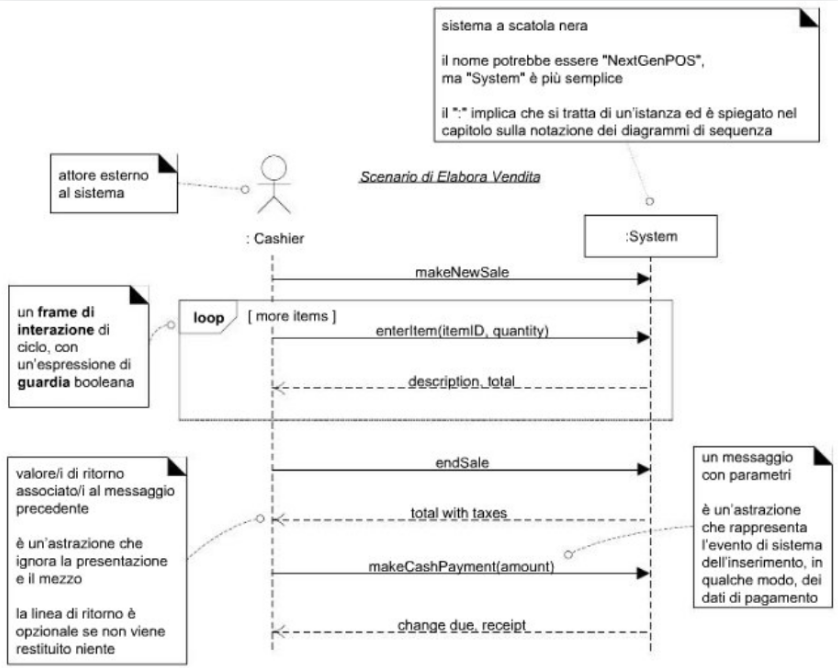
\includegraphics[scale=0.35]{images/SSD.png}
    \end{center}
\pagebreak
    \begin{itemize}
        \item [$\Rightarrow$] \textit{makeNewSale}: il cassiere inizia una nuova vendita;
        \item [$\Rightarrow$] \textit{enterItem}: il cassiere inserisce il codice identificativo di un articolo;
        \item [$\Rightarrow$] \textit{endSale}: il cassiere indica di aver terminato l'inserimento degli articoli acquistati;
        \item [$\Rightarrow$] \textit{makeCashPayment}: il cassiere indica che il cliente sta pagando in contanti e inserisce l'importo offerto dal cliente. 
    \end{itemize}


}

\subsubsection{Un SSD mostra:}

\begin{itemize}
    \item [$\Rightarrow$] L'attore primario del Caso d'Uso;
    \item [$\Rightarrow$] Il sistema in discussione;
    \item [$\Rightarrow$] I passi che rappresentano le interazioni tra il sistema e l'attore.
\end{itemize}

\nt{Le interazioni sono mostrate come messaggi con parametri.}

\subsection{Notazione}

\subsubsection{\fancyglitter{Semplice diagramma di sequenza:}}

\begin{center}
    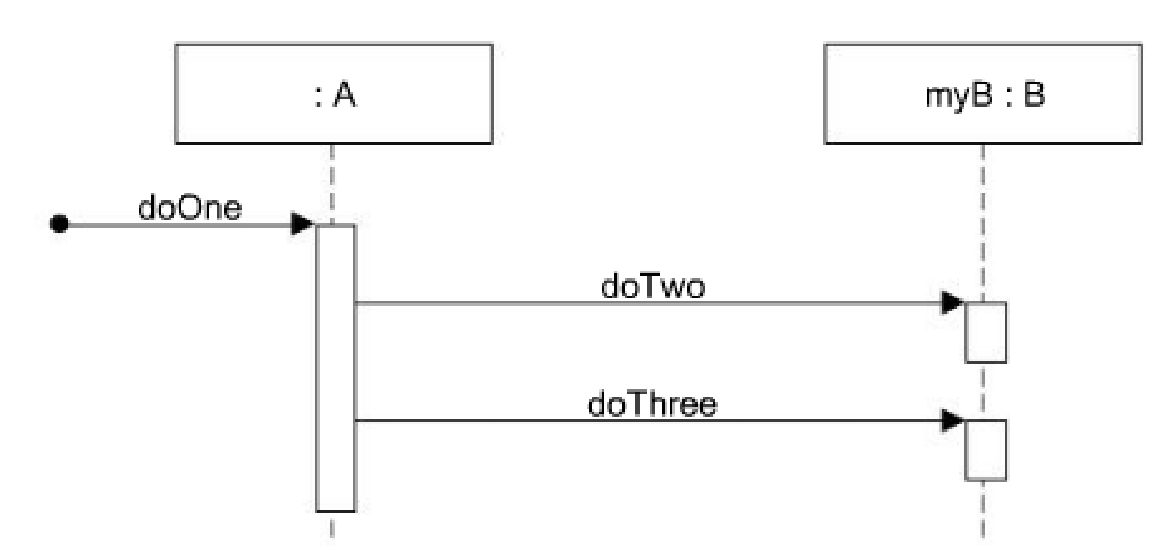
\includegraphics[scale=0.33]{images/Notazione SSD.png}
\end{center}

\subsubsection{\fancyglitter{Mostrare il risultato di ritorno:}}

\begin{center}
    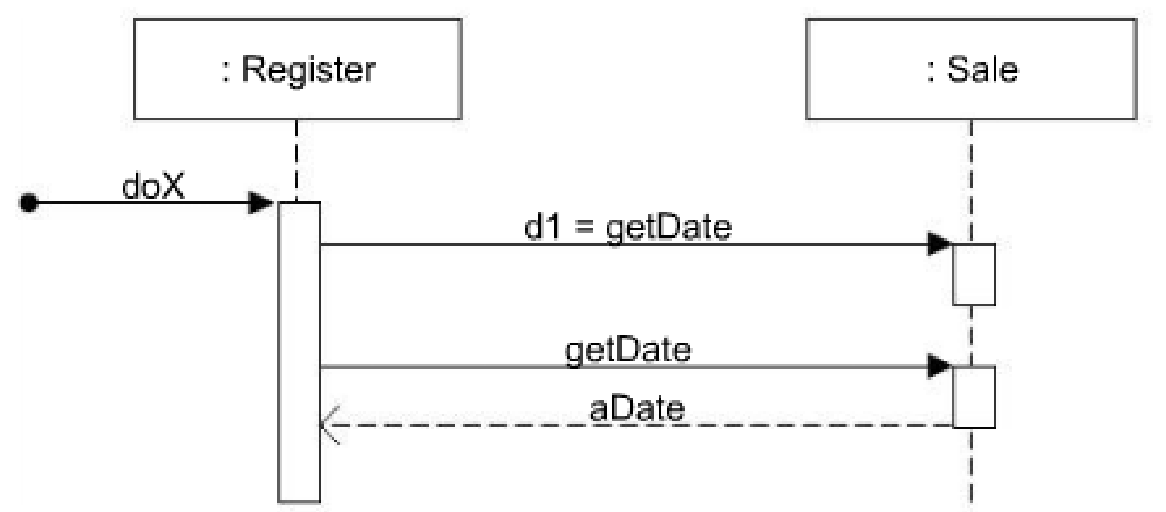
\includegraphics[scale=0.33]{images/Notazione SSD2.png}
\end{center}

\subsubsection{\fancyglitter{Frame di UML:}}

\begin{center}
    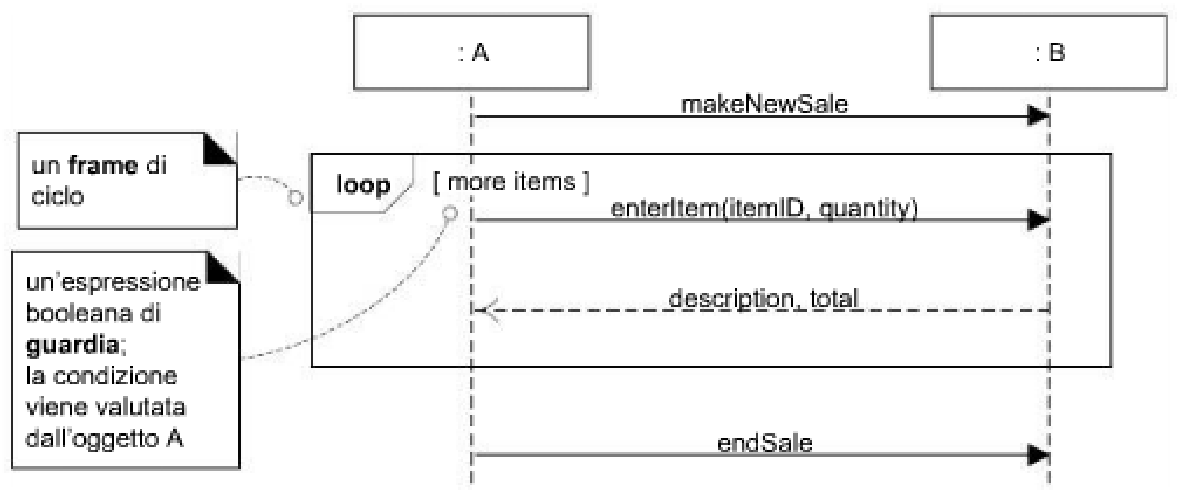
\includegraphics[scale=0.33]{images/Notazione SSD3.png}
\end{center}

\subsubsection{\fancyglitter{Operatori comuni per i frame UML:}}

\begin{center}
    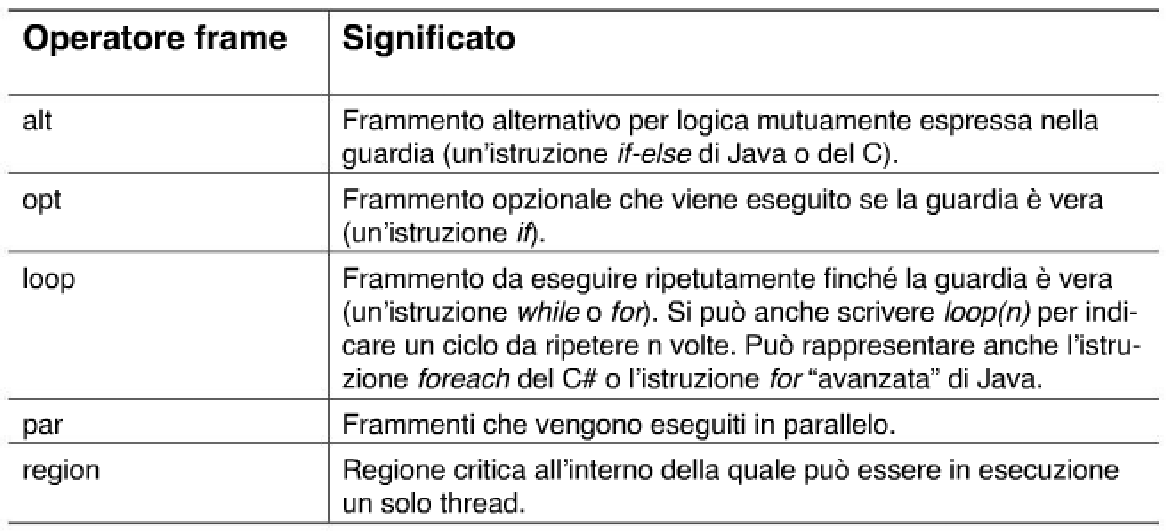
\includegraphics[scale=0.33]{images/Notazione SSD4.png}
\end{center}

\subsubsection{\fancyglitter{Annidamento di frame:}}

\begin{center}
    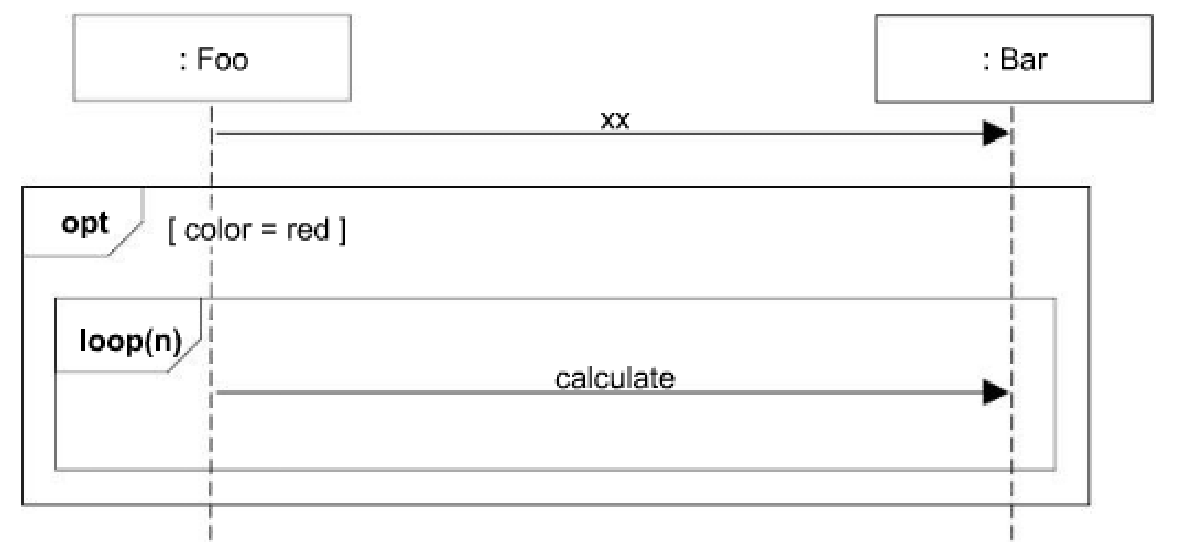
\includegraphics[scale=0.33]{images/Notazione SSD5.png}
\end{center}

\section{Contratti}
\label{contratti}

\subsection{Pre-condizioni e Post-condizioni}

\dfn{I contratti delle operazioni}{
    I contratti usano \newfancyglitter{pre-condizioni} e \newfancyglitter{post-condizioni} per descrivere nel
    dettaglio i cambiamenti agli oggetti in un Modello di Dominio.

    \paragraph{Punto di vista:}
    \begin{itemize}
        \item [\textcolor{dkgreen}{\checkmark}] Concettuale.
        \item [\textcolor{red}{\XSolidBrush}] Implementativo.
    \end{itemize}
}

\nt{Possono essere considerati parte del Modello dei Casi d'Uso, ma non sono
menzionati esplicitamente in UP.}

\ex{Contratto}{

    \begin{center}
        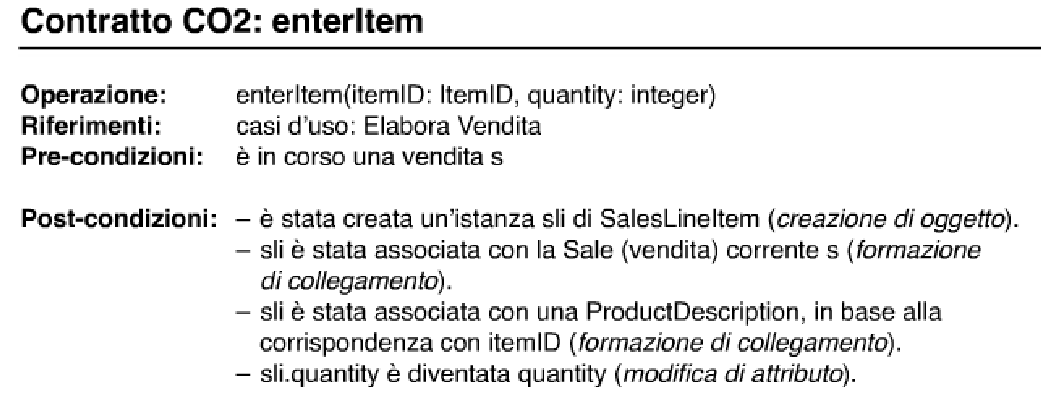
\includegraphics[scale=0.35]{images/Contratto.png}
    \end{center}
}

\subsubsection{Template di un contratto:}

\begin{itemize}
    \item [$\Rightarrow$] \fancyglitter{Operazione}: Nome e parametri dell'operazione;
    \item [$\Rightarrow$] \fancyglitter{Riferimenti}: Casi d'Uso in cui può verificarsi l'operazione;
    \item [$\Rightarrow$] \fancyglitter{Pre-condizioni}: Stato del sistema prima dell'operazione. Sono ipotesi non banali;
    \item [$\Rightarrow$] \fancyglitter{Post-condizioni}: Stato del sistema dopo l'operazione. 
\end{itemize}

\dfn{Post-condizioni}{
    Le \newfancyglitter{post-condizioni} descrivono i cambiamenti nello stato degli oggetti
    del Modello di Dominio. I cambiamenti comprendono:
    
    \begin{itemize}
        \item [$\Rightarrow$] Oggetti creati;
        \item [$\Rightarrow$] Collegamenti formati;
        \item [$\Rightarrow$] Collegamenti rotti;
        \item [$\Rightarrow$] Attributi modificati.
    \end{itemize}

}

\nt{Le post-condizioni sono osservazioni al termine dell'operazione.
Ci si concentra sul "cosa", ma non sul "come".}

\dfn{Pre-condizioni}{
    Le \newfancyglitter{pre-condizioni} sono ipotesi sullo stato del sistema
    prima dell'operazione. Sono condizioni che devono essere vere
    prima che l'operazione possa essere eseguita.
}

\nt{Le pre-condizioni sono una descrizione sintetica sullo stato
di avanzamento del Caso d'Uso.}

\subsection{Scrivere contratti}

\subsubsection{Si procede così:}

\begin{enumerate}
    \item Si identificano le operazioni dagli SSD;
    \item Si crea un contratto per le operazioni complesse
    o i cui effetti sono sottili (non chiari dai Casi d'Uso);
    \item Si scrivono le pre-condizioni e le post-condizioni:
    \begin{itemize}
        \item [$\Rightarrow$] creazione o cancellazione di oggetti;
        \item [$\Rightarrow$] formazione o rottura di collegamenti;
        \item [$\Rightarrow$] modifica di attributi.
    \end{itemize}
\end{enumerate}

\nt{Ogni operazione può avere una componente di:

\begin{itemize}
    \item [$\Rightarrow$] \fancyglitter{Trasformazione}: modifica lo stato del sistema;
    \item [$\Rightarrow$] \fancyglitter{Interrogazione}: non modifica lo stato del sistema, vengono restituiti valori.
\end{itemize}

Un'operazione ha post-condizioni solo se è di trasformazione, mentre
non le ha se è di interrogazione.
}

\qs{}{Bisogna scrivere un contratto per ogni evento di sistema trovato nel SSD?}

\paragraph{Risposta:} Non è necessario, si considerano solo quelli più complessi.
\paragraph{}
\qs{}{Se si scoprono nuove classi, attributi, si possono aggiungere nel modello di dominio?}

\paragraph{Risposta:} Sì, UP è incrementale.
\paragraph{}
\qs{}{Le post-condizioni devono essere in ogni momento le pi`u complete possibili?}

\paragraph{Risposta:} Non è necessario.

\definecolor{chaptergrey}{rgb}{1,0.75,0}
\ifnum\layout=2 
    \fancyhf{}      
    \renewcommand{\headrulewidth}{0pt}
    \renewcommand{\chaptermark}[1]{\markboth{#1}{}}

    \fancyhead[LE]{\nouppercase{\textbf{\textcolor{chaptergrey}{\chaptername}}~ \thechapter~ |~ \leftmark}}
    \fancyhead[RO]{\nouppercase{ \rightmark}}
    \fancyfoot[LE,RO]{\thepage}
    \fancypagestyle{plain}{         
    \fancyhf{}
    \fancyfoot[LE,RO]{\thepage}}    
 \else          
    \renewcommand{\headrulewidth}{0pt}
    \fancyhf{}                  
    \fancyhead[C]{\nouppercase{ \leftmark}}
    \fancyfoot[C]{\thepage}
\fi

\chapter{Architettura del software}

\section{Architettura logica}

\dfn{Architettura}{
    La progettazione OO è  basata su diversi strati architetturali,
    come uno strati UI, uno strato di logica applicativa (o "del dominio") e così via.
}

\nt{L'architettura può essere mostrata sotto forma di diagrammi UML.}

\ex{Package UML}{
    \begin{center}
        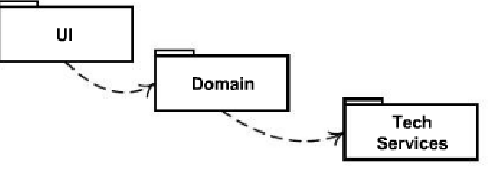
\includegraphics[scale=0.5]{images/PackageUML.png}
    \end{center}
}

\dfn{Architettura logica}{
    L'\newfancyglitter{architettura logica} di un sistema
    software è la macro-organizzazione su larga scala delle 
    classi in package (o namespace), sottoinsiemi e strati.
}

\nt{Non vengono prese decisioni su come gli elementi sono distribuiti
sui processi o sui vari computer fisici di una rete (\fancyglitter{platform independent architecture}).}

\cor{Layer (o Strato)}{
    Un layer è un gruppo di classi software, packages, sottosistemi con responsabilità
    condivisa su un aspetto importante del sistema.
}

\subsubsection{Gli strati comprendono:}

\begin{itemize}
    \item [$\Rightarrow$] \fancyglitter{UI (User Interface)}: strato che si occupa dell'interazione con l'utente;
    \item [$\Rightarrow$] \fancyglitter{Application logic} (o "domain object"): oggetti software che rappresentano concetti di dominio;
    \item [$\Rightarrow$] \fancyglitter{Technical services}: oggetti e sottosistemi che forniscono servizi tecnici (es. persistenza, sicurezza, ecc.);
\end{itemize}

\subsubsection{Rappresentazioni di strati:}
    \begin{figure}[!h]
        \centering
        \subfloat[Packeges UML]{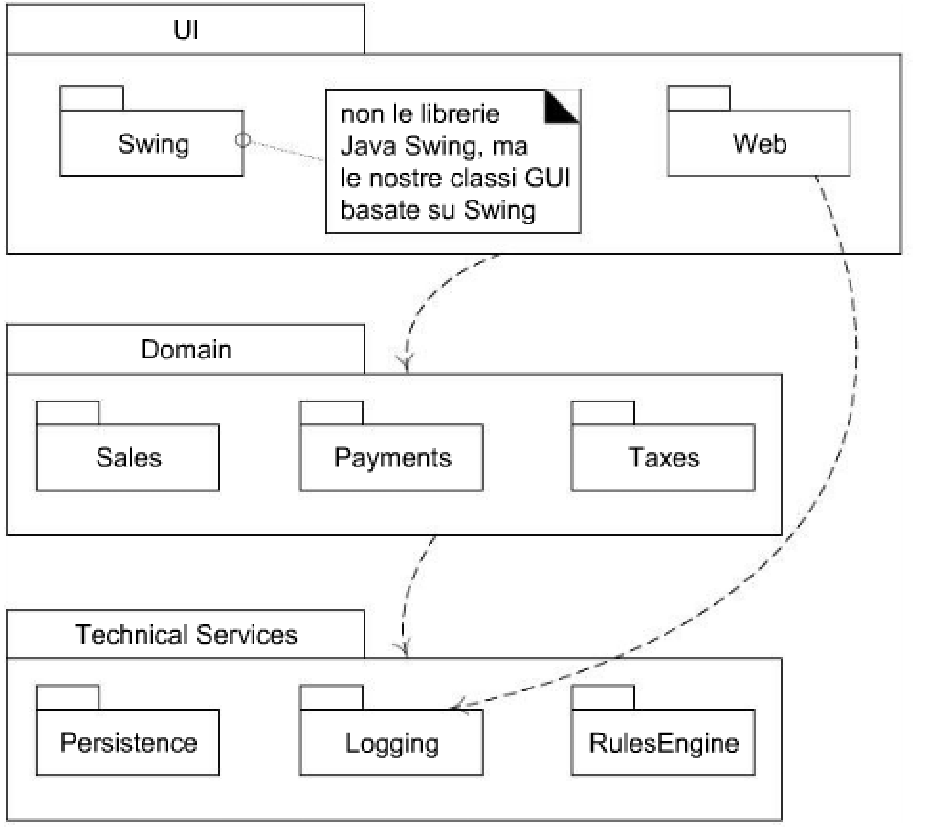
\includegraphics[scale = 0.25]{images/UMLPackage.png}} 
        \subfloat[Relativo codice]{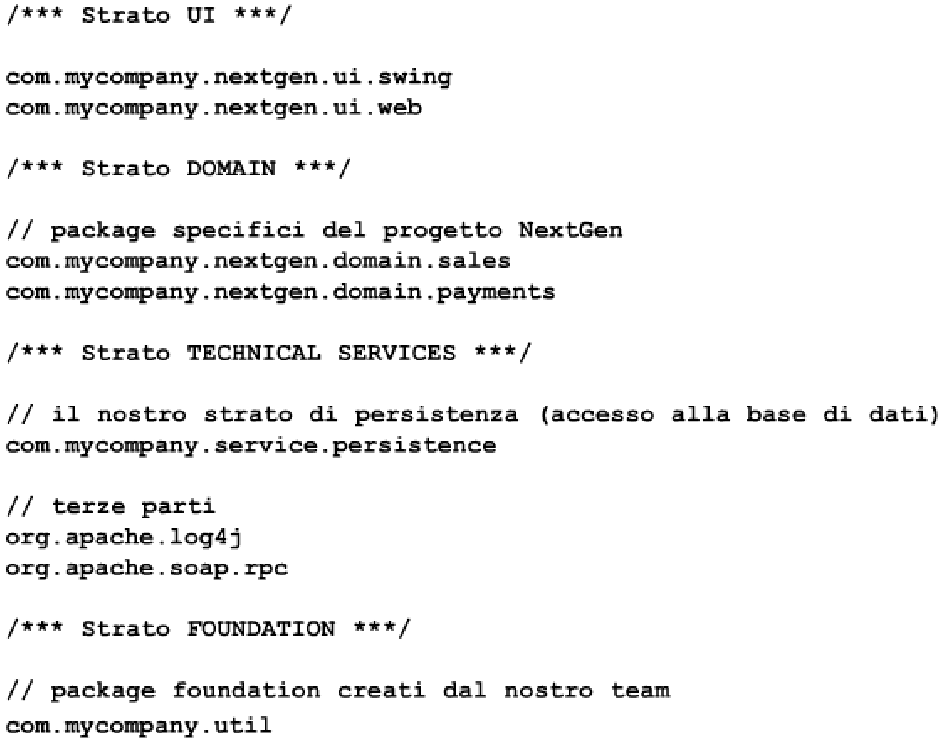
\includegraphics[scale = 0.25]{images/PackageCode.png}}
    \end{figure}

\dfn{Architettura a strati}{
    L'obiettivo di un'\newfancyglitter{architettura a strati} è la suddivisione di un sistema complesso
    in un insieme di elementi software che possano essere sviluppati e modificati in modo indipendente.
}

\cor{Separation of concerns}{
    La separazione degli interessi:

    \begin{itemize}
        \item [$\Rightarrow$] Riduce l'accoppiamento e le dipendenze;
        \item [$\Rightarrow$] Aumenta la possibilità di riuso;
        \item [$\Rightarrow$] Facilita la manutenzione e l'evoluzione del sistema;
        \item [$\Rightarrow$] Aumenta la chiarezza.
    \end{itemize}
}

\cor{Alta coesione}{
    In uno strato le responsabilità degli oggetti devono essere fortemente
    collegate tra loro, ma non essere mischiate con quelle di altri strati.
}

\nt{Questi due principi verranno ripresi in GRASP, vedi capitolo \ref{GRASP}.}

\pagebreak

\ex{Architettura a strati}{
    \begin{center}
        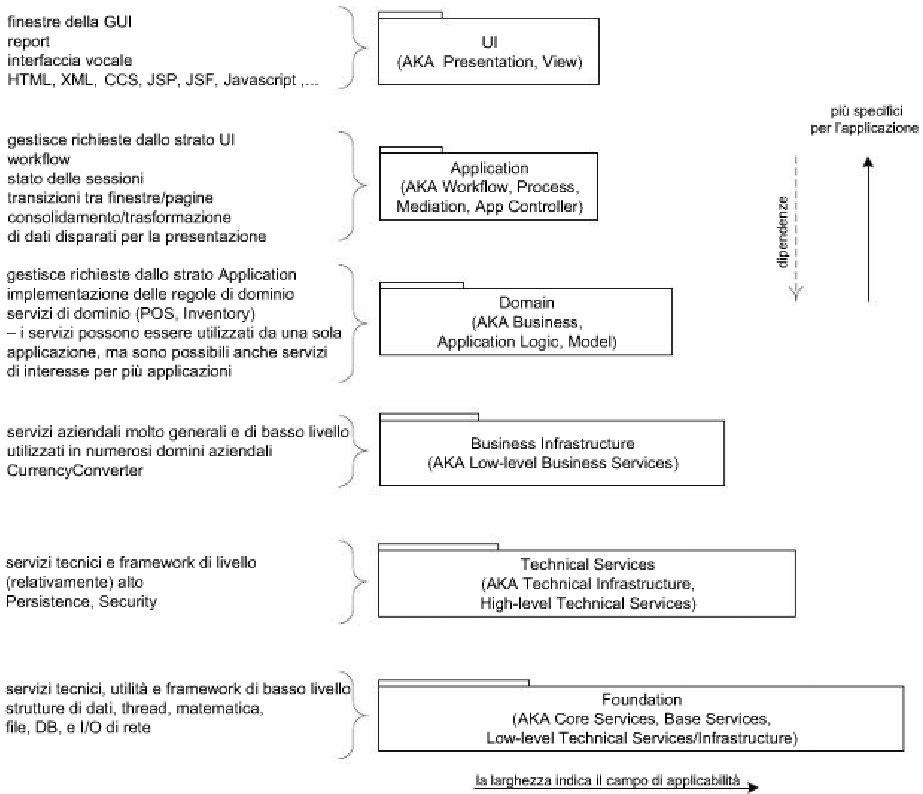
\includegraphics[scale=0.45]{images/Architettura a strati.png}
    \end{center}

}


\section{Strato del dominio}

\qs{}{Come va progettata la logica applicativa con gli oggetti?}

\paragraph{Risposta:} Si creano oggetti software con nomi e informazioni simili
al Dominio del mondo reale e assegnare a essi le responsabilità della logica applicativa.

\dfn{Oggetto del Dominio}{
    Un \newfancyglitter{oggetto del dominio} è un oggetto software che rappresenta un concetto del dominio del problema.

    Ha una logica applicativa o di business correlata.
}

\nt{Ispirandosi al Modello del Dominio si ha un basso salto rappresentazionale che
rende più facile e veloce l'implementazione.}

\ex{Strato di Dominio e Modello di Dominio}{

    \begin{center}
        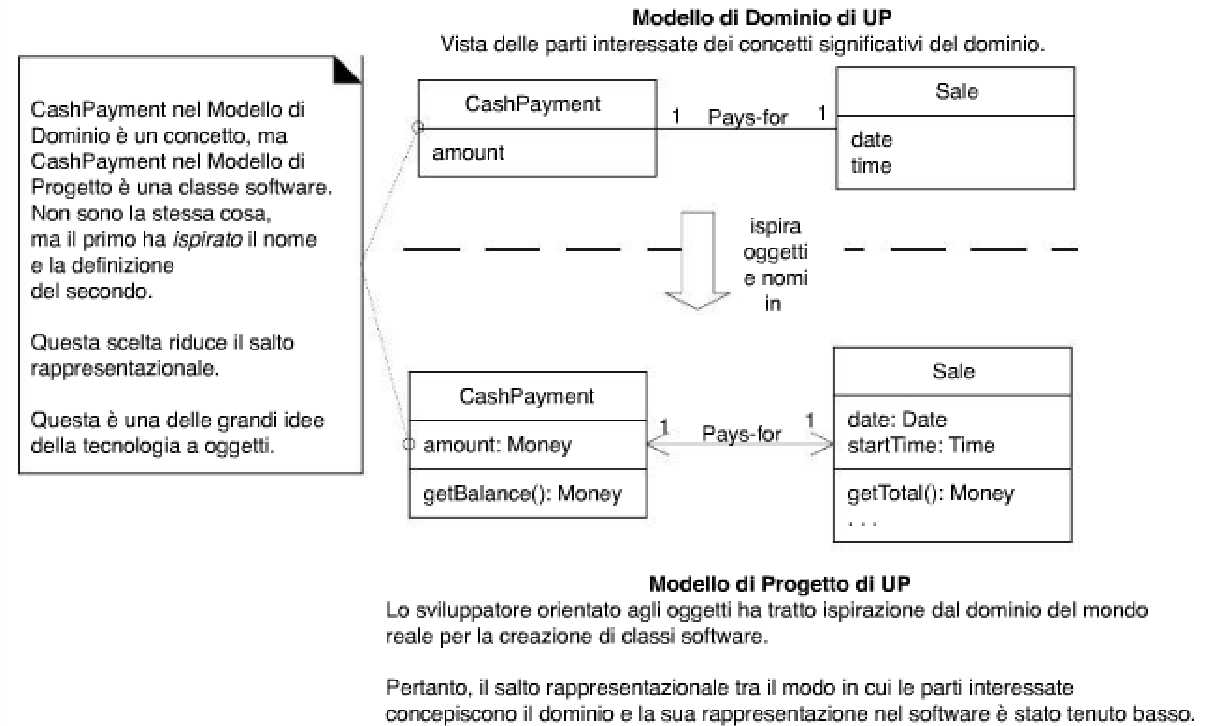
\includegraphics[scale=0.35]{images/Modello.png}
    \end{center}
}

\ex{Strati e Partizioni}{
    \begin{center}
        \includegraphics[scale=0.35]{images/Strati e Partizioni.png}
    \end{center}
}

\section{Separazione Modello-Vista}

\dfn{Principio di separazione Modello-Vista}{
    \begin{itemize}
        \item [\textcolor{red}{\XSolidBrush}] Non relazionare o accoppiare oggetti non UI con oggetti UI.
        \item [\textcolor{red}{\XSolidBrush}] Non incapsulare la logica applicativa in metodi UI.
        \item [\textcolor{green}{\Checkmark}] Le finestre appartengono a una specifica applicazione, mentre
        gli oggetti non UI possono venire riutilizzati in nuove applicazioni o associati a nuove interfacce.
        \item [\textcolor{green}{\Checkmark}] Gli oggetti UI inizializzano elementi UI, ricevono eventi UI e
        delegano le richieste della logica dell'applicazione agli oggetti non UI.
    \end{itemize}
}

\nt{
    \begin{itemize}
        \item [$\Rightarrow$] Il Modello è lo strato degli oggetti del dominio;
        \item [$\Rightarrow$] La Vista è lo strato UI.
    \end{itemize}

    Questo principio è alla base del pattern MVC\footnote{Visto nel corso "Programmazione III".}.
}

\subsubsection{Ulteriori considerazioni:}

\begin{itemize}
    \item [$\Rightarrow$] Le classi di dominio incapsulano le informazioni e il comportamento della logica applicativa;
    \item [$\Rightarrow$] Le classi della vista sono leggere, sono responsabili dell'inpute e dell'output, ma non mantengono dati.
\end{itemize}

\subsubsection{Vantaggi:}

\begin{itemize}
    \item [$\Rightarrow$] Favorire la definizione coesa dei modelli;
    \item [$\Rightarrow$] Consentire lo sviluppo separaro;
    \item [$\Rightarrow$] Minimizzare l'impatto sullo strato del dominio;
    \item [$\Rightarrow$] Consentire di connettere facilmente nuove viste;
    \item [$\Rightarrow$] Consentire l'esecuzione dello strato di modello indipendentemente dallo strato UI;
    \item [$\Rightarrow$] Consentire un \textit{porting} facile dello strato di modello a un altro framework UI.
\end{itemize}

\ex{SSD e UI}{
    \begin{center}
        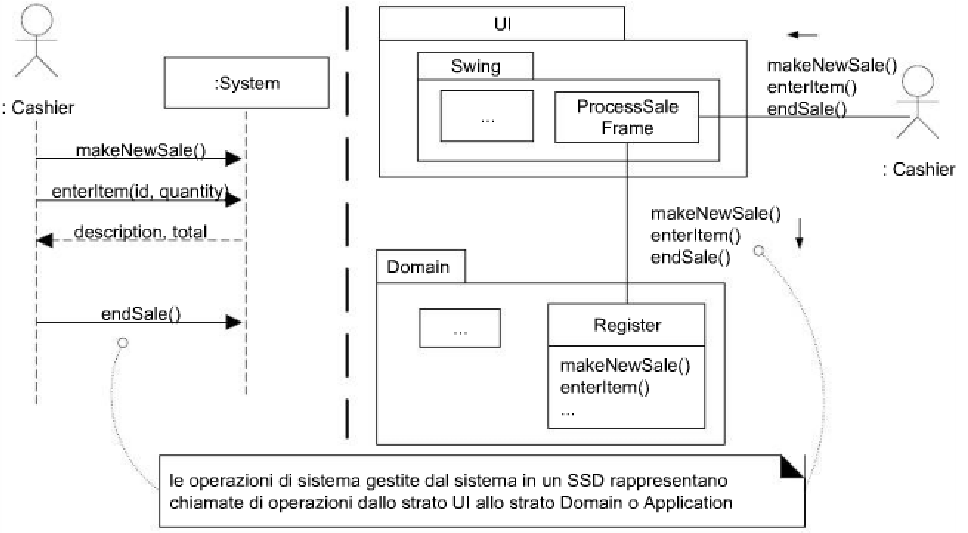
\includegraphics[scale=0.3]{images/SSD e UI.png}
    \end{center}
}
\definecolor{chaptergrey}{rgb}{1,0.75,0.8}
\ifnum\layout=2 
    \fancyhf{}      
    \renewcommand{\headrulewidth}{0pt}
    \renewcommand{\chaptermark}[1]{\markboth{#1}{}}

    \fancyhead[LE]{\nouppercase{\textbf{\textcolor{chaptergrey}{\chaptername}}~ \thechapter~ |~ \leftmark}}
    \fancyhead[RO]{\nouppercase{ \rightmark}}
    \fancyfoot[LE,RO]{\thepage}
    \fancypagestyle{plain}{         
    \fancyhf{}
    \fancyfoot[LE,RO]{\thepage}}    
 \else          
    \renewcommand{\headrulewidth}{0pt}
    \fancyhf{}                  
    \fancyhead[C]{\nouppercase{ \leftmark}}
    \fancyfoot[C]{\thepage}
\fi

\chapter{Diagrammi di interazione e di classe UML}

\section{Verso la progettazione a oggetti}

\qs{}{Come si progetta a oggetti?}

\begin{itemize}
    \item [$\Rightarrow$] \fancyglitter{Codifica}: si progetta mentre
    si codifica;
    \item [$\Rightarrow$] \fancyglitter{Disegno, poi codifica}: si
    disegnano i diagrammi UML e poi si codifica;
    \item [$\Rightarrow$] \fancyglitter{Solo disegno}: si disegnano i
    diagrammi UML e lo strumento genera ogni cosa da essi.
\end{itemize}

\nt{Solitamente si sceglie di disegnare e poi codificare.}

\subsection{Modellazione dinamica e statica}

\dfn{Modelli dinamici}{Rappresentano il comportamento del sistema,
la collaborazione tra oggetti per realizzare dei Casi d'Uso. Di solito
si utilizzano i diagrammi di interazione UML.}

\dfn{Modelli statici}{
    Servono per definire package, nomi delle classi, attributi e
    firme di operazioni. Di solito si utilizzano i diagrammi delle
    classi UML.
}

\nt{Solitamente si creano in parallelo sia i modelli dinamici che
statici.}
\pagebreak
\ex{Modelli statici e dinamici}{
    \begin{center}
        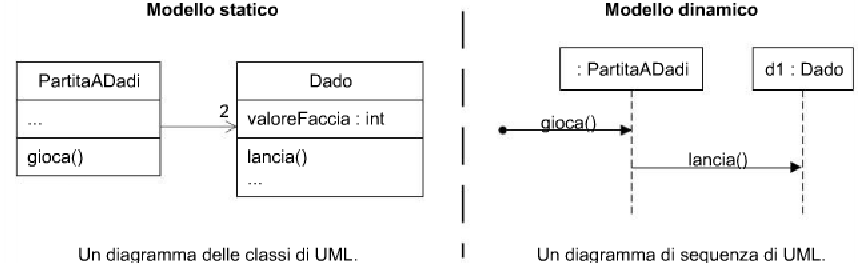
\includegraphics[scale=0.45]{images/Modelli statici e dinamici.png}
    \end{center}
}

\begin{itemize}
    \item [$\Rightarrow$] La maggior parte del lavoro utile e difficile
    avviene nel disegno dei diagrammi di interazione (o di sequenza);
    \item [$\Rightarrow$] Durante la modellazione dinamica si pensa
    a quali oggetti devono esistere e a come collaborano tra loro;
    \item [$\Rightarrow$] Per la modellazione dinamica si fa riferimento
    ai principi GRASP\footnote{Vedi capitolo \ref{GRASP}.}.
\end{itemize}

\subsubsection{Le domande che ci si deve porre sono:}

\begin{itemize}
    \item [$\Rightarrow$] \fancyglitter{Quali} sono le responsabilità
    dell'oggetto?
    \item [$\Rightarrow$] \fancyglitter{Chi} collabora con chi?
    \item [$\Rightarrow$] \fancyglitter{Quali} design pattern devono essere applicati?
\end{itemize}

\subsubsection{La progettazione a oggetti richiede la conoscenza di:}

\begin{itemize}
    \item [$\Rightarrow$] \fancyglitter{Design pattern};
    \item [$\Rightarrow$] \fancyglitter{Principi di assegnazione delle responsabilità}.
\end{itemize}

\section{Diagrammi di interazione}

\dfn{Interazione}{
    Un'\newfancyglitter{interazione} è una specifica di come alcuni
    oggetti si scambiano messaggi nel tempo per eseguire un compito nell'ambito
    di un certo contesto.
}

\nt{Il termine diagramma di interazione si riferisce a due tipi di diagrammi:
\begin{itemize}
    \item [$\Rightarrow$] \fancyglitter{Diagrammi di sequenza};
    \item [$\Rightarrow$] \fancyglitter{Diagrammi di comunicazione}.

\end{itemize}

In questo corso ci concentreremo sui diagrammi di sequenza.
}

\subsubsection{Caratteristiche dei diagrammi di sequenza:}

\begin{itemize}
    \item [$\Rightarrow$] Un'\fancyglitter{interazione} è motivata dalla necessità
    di eseguire un \fancyglitter{compito};
    \item [$\Rightarrow$] Un \fancyglitter{compito} è rappresentato da un 
    \fancyglitter{messaggio} che dà inizio all'interazione (messaggio trovato);
    \item [$\Rightarrow$] Il \fancyglitter{messaggio} è inviato a un oggetto designato
    come \fancyglitter{responsabile} del compito;
    \item [$\Rightarrow$] L'oggetto \fancyglitter{responsabile} collabora con
    altri oggetti (\fancyglitter{partecipanti}) per eseguire il compito;
    \item [$\Rightarrow$] Ciascun \fancyglitter{partecipante} svolge un proprio
    \fancyglitter{ruolo} nell'interazione;
    \item [$\Rightarrow$] La \fancyglitter{collaborazione} avviene mediante 
    \fancyglitter{messaggi} scambiati tra gli oggetti;
    \item [$\Rightarrow$] Ciascun messaggio è una richiesta che un oggetto fa a un altro
    oggetto di eseguire un'\fancyglitter{operazione}.
\end{itemize}

\subsubsection{Vantaggi e svantaggi dei diagrammi di sequenza:}

\begin{itemize}
    \item [\textcolor{green}{\checkmark}] Mostrano chiaramente la sequenza 
    dell'ordinamento temporale dei messaggi.
    \item [\textcolor{red}{\XSolidBrush}] Costringono a estendersi verso destra
    quando si aggiungono nuovi oggetti.
\end{itemize}

\ex{Diagrammi di sequenza}{
    \begin{center}
        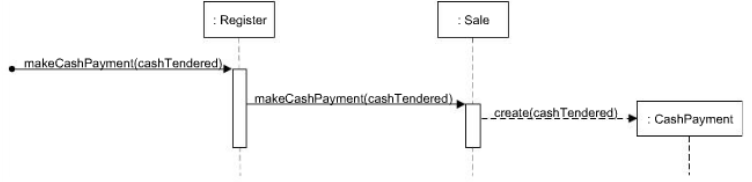
\includegraphics[scale=0.45]{images/Diagramma di sequenza.png}
    \end{center}
}

\subsection{Diagrammi di sequenza del design (DSD)}

\dfn{Design Sequence Diagram (DSD)}{
    Un \newfancyglitter{diagramma di sequenza} di progetto è un diagramma
    di sequenza utilizzato da un punto di vista software o di progetto.
}

\nt{In UP l'insieme di tutti i DSD fa parte del modello di progetto.}

\ex{Notazione di DSD: partecipanti}{
    \begin{center}
        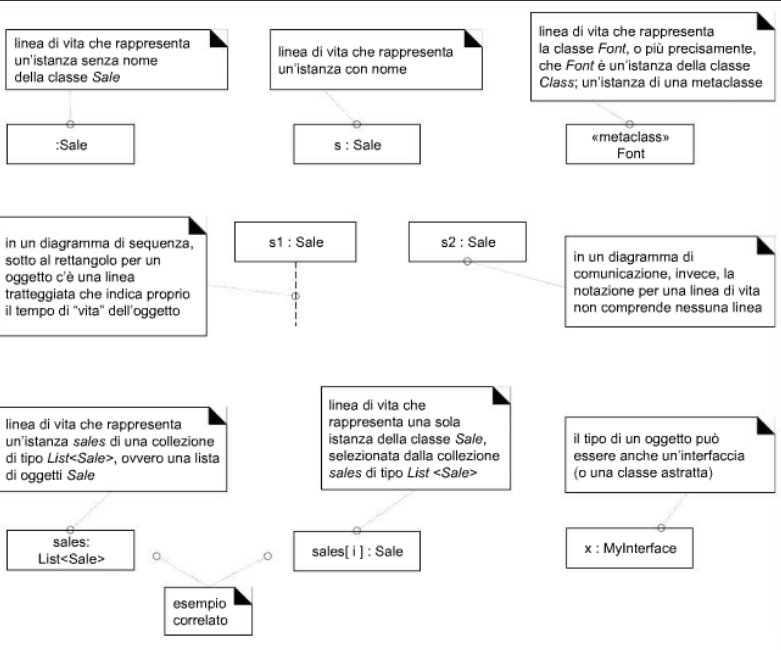
\includegraphics[scale=0.35]{images/Notazione di DSD.png}
    \end{center}
}

\dfn{Singleton}{
    Un \newfancyglitter{singleton} è un pattern nel quale da una classe viene istanziata una sola istanza.
}

\ex{Notazione di DSD: singleton}{
    \begin{center}
        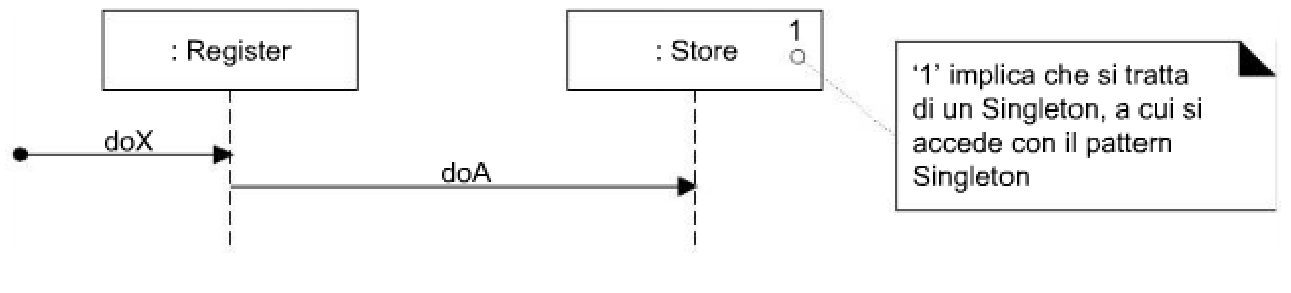
\includegraphics[scale=0.25]{images/Singleton.png}
    \end{center}
}

\ex{Notazione di DSD: messaggi}{
    \begin{center}
        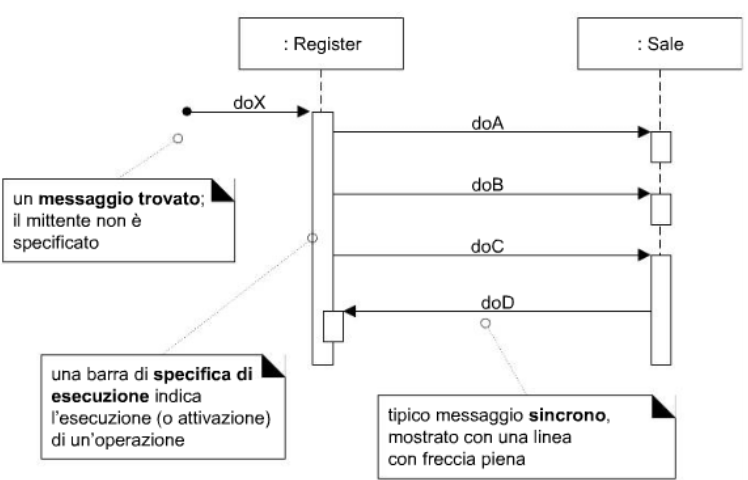
\includegraphics[scale=0.35]{images/Messaggi.png}
    \end{center}
}

\ex{Notazione di DSD: self (this)}{
    \begin{center}
        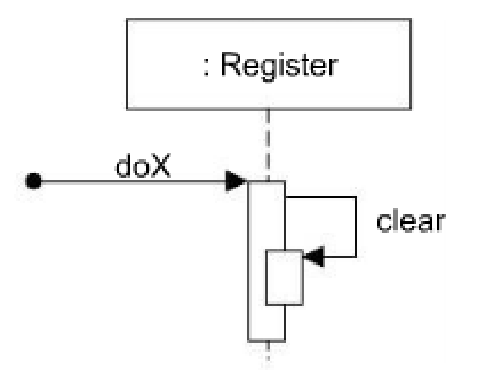
\includegraphics[scale=0.35]{images/Self.png}
    \end{center}
}

\ex{Notazione di DSD: creazione di istanze}{
    \begin{center}
        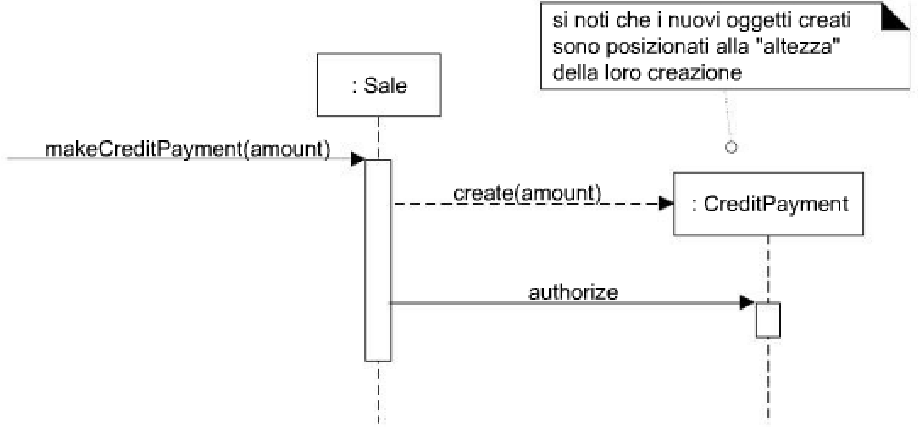
\includegraphics[scale=0.35]{images/Creazione di istanze.png}
    \end{center}
}

\ex{Notazione di DSD: distruzione di oggetti}{
    \begin{center}
        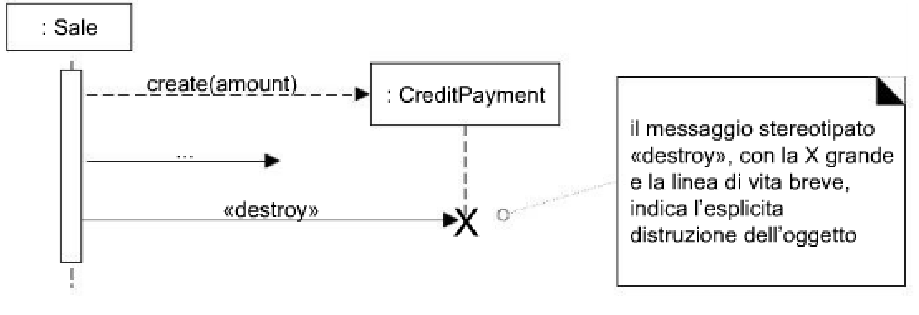
\includegraphics[scale=0.35]{images/Distruzione di oggetti.png}
    \end{center}
}
\pagebreak
\ex{Notazione di DSD: collegamenti}{
    \begin{center}
        \includegraphics[scale=0.35]{images/Collegamento1.png}
        \includegraphics[scale=0.35]{images/Collegamento2.png}
    \end{center}

}

\ex{Notazione di DSD: frame}{
    \begin{center}
        \includegraphics[scale=0.35]{images/Frame.png}
    \end{center}
}
\pagebreak
\ex{Notazione di DSD: condizionale}{
    \begin{center}
        \includegraphics[scale=0.35]{images/Condizioni.png}
    \end{center}
}

\ex{Notazione di DSD: condizionale mutualmente esclusivo}{
    \begin{center}
        \includegraphics[scale=0.35]{images/Alt.png}
    \end{center}
}

\ex{Notazione di DSD: iterazione su una collezione}{
    \begin{center}
        \includegraphics[scale=0.35]{images/Iterazione.png}
    \end{center}
}

\pagebreak

\ex{Notazione di DSD: correlare diagrammi di interazione}{
    \begin{center}
        \includegraphics[scale=0.4]{images/Correlare.png}
    \end{center}
}

\ex{Notazione di DSD: invocare metodi statici}{
    \begin{center}
        \includegraphics[scale=0.35]{images/Static.png}
    \end{center}
}

\nt{Nel caso di invocazione di metodi statici l'oggetto ricevente è
un'istanza di una meta-classe.}

\pagebreak

\ex{Notazione di DSD: chiamate sincrone e asincrone}{
    \begin{center}
        \includegraphics[scale=0.45]{images/Chiamate.png}
    \end{center}
}
\pagebreak
\section{Diagrammi delle classi}

\subsection{Diagrammi di classe del design (DCD)}

\dfn{Design Class Diagram (DCD)}{
    Un \newfancyglitter{diagramma delle classi} di progetto è un diagramma
    delle classi utilizzato da un punto di vista software o di progetto.
}


\nt{In UP l'insieme di tutti i DCD fa parte del modello di progetto.}

\ex{Notazione generale di DCD}{
    \begin{center}
        \includegraphics[scale=0.5]{images/Generale.png}
    \end{center}
}

\nt{
    \begin{itemize}
        \item [$\Rightarrow$] \fancyglitter{$+$} indica un attributo pubblico;
        \item [$\Rightarrow$] \fancyglitter{$-$} indica un attributo privato;
        \item [$\Rightarrow$] \fancyglitter{\#} indica un attributo protetto;
        \item [$\Rightarrow$] \fancyglitter{\textasciitilde} indica un attributo package.
    \end{itemize}
}

\ex{Notazione di DCD: attributi}{
    \begin{center}
        \includegraphics[scale=0.45]{images/Attributi.png}
    \end{center}
}

\nt{Se non viene specificata la visibilità di un attributo si intende
che esso sia privato.}

\ex{Notazione di DCD: parole chiave}{
    \begin{center}
        \includegraphics[scale=0.3]{images/Parole chiave.png}
    \end{center}
}
\dfn{Stereotipi}{
    Gli \newfancyglitter{stereotipi} sono un raffinamento di un concetto
    di modellazione esistente.
}

\ex{Notazione di DCD: stereotipi}{
    \begin{center}
        \includegraphics[scale=0.25]{images/Stereotipi.png}
    \end{center}
}

\dfn{Generalizzazione}{
    La \newfancyglitter{generalizzazione} è una relazione tassonomica
    tra una classe più generale e una classe più specifica. Ogni istanza
    della classe specifica è anche un'istanza della classe generale.
}

\nt{La generalizzazione implica \fancyglitter{ereditarietà} nei linguaggi OO.}

\dfn{Linee di dipendenza}{
    Una \newfancyglitter{linea di dipendenza} è una relazione tra due
    classi che indica che un cambiamento nella classe dipendente può
    influenzare la classe dipendente.
}

\ex{Notazione di DCD: dipendenza}{
    \begin{center}
        \includegraphics[scale=0.45]{images/Dipendenza.png}
    \end{center}
}

\nt{È importante mantenere un basso accoppiamento tra le classi.}

\subsubsection{Esistono varie tipologie di dipendenze:}

\begin{itemize}
    \item [$\Rightarrow$] Avere un attributo del tipo del fornitore;
    \item [$\Rightarrow$] Inviare un messaggio al fornitore;
    \item [$\Rightarrow$] Ricevere un parametro del tipo del fornitore;
    \item [$\Rightarrow$] Il fornitore è una superclasse o un'interfaccia implementata.
\end{itemize}

\dfn{Interfacce}{
    Un'\newfancyglitter{interfaccia} è un contratto tra un fornitore
    e un cliente. Un cliente può invocare i metodi definiti nell'interfaccia.
    Si hanno due notazioni:
    \begin{itemize}
        \item [$\Rightarrow$] \newfancyglitter{Notazione a pallina} (lollipop),
        indica che una classe X implementa (fornisce) un'interfaccia Y;
        \item [$\Rightarrow$] \newfancyglitter{Notazione a semicerchio} (socket),
        indica che una classe X richiede (usa) un'interfaccia Y.
    \end{itemize}
}
\pagebreak
\ex{Notazione di DCD: composizione}{
    \begin{center}
        \includegraphics[scale=0.35]{images/Composizione.png}
    \end{center}
}

\ex{Notazione di DCD: singleton}{
    \begin{center}
        \includegraphics[scale=0.33]{images/Singleton2.png}
    \end{center}
}

\ex{Notazione di DCD: tipi a template}{
    \begin{center}
        \includegraphics[scale=0.35]{images/Template.png}
    \end{center}
}

\definecolor{chaptergrey}{rgb}{0,0.13, 0.38}
\ifnum\layout=2 
    \fancyhf{}      
    \renewcommand{\headrulewidth}{0pt}
    \renewcommand{\chaptermark}[1]{\markboth{#1}{}}

    \fancyhead[LE]{\nouppercase{\textbf{\textcolor{chaptergrey}{\chaptername}}~ \thechapter~ |~ \leftmark}}
    \fancyhead[RO]{\nouppercase{ \rightmark}}
    \fancyfoot[LE,RO]{\thepage}
    \fancypagestyle{plain}{         
    \fancyhf{}
    \fancyfoot[LE,RO]{\thepage}}    
 \else          
    \renewcommand{\headrulewidth}{0pt}
    \fancyhf{}                  
    \fancyhead[C]{\nouppercase{ \leftmark}}
    \fancyfoot[C]{\thepage}
\fi

\chapter{Pattern GRASP}
\label{GRASP}

\section{Responsability-Driven Development}

\dfn{Responsability-Driven Development (RDD)}{
    L'approccio complessivo al fare la modellazione per la programmazione
    OO si basa sulla metafore della \newfancyglitter{progettazione guidata dalle responsabilità} (RDD),
    che è un modo di pensare a come assegnare le responsabilità agli oggetti
    che collaborano.
}

\cor{responsabilità}{
    Per responsabilità si intende un'astrazione di ciò che fa o rappresenta
    un oggetto o un componente software. Le responsabilità sono di due tipi:
    \begin{itemize}
        \item [$\Rightarrow$] Di fare;
        \item [$\Rightarrow$] Di conoscere.
    \end{itemize}
}

\nt{In UML la responsabilità è un \fancyglitter{contratto} o 
un \fancyglitter{obbligo} di un oggetto.}

\subsection{Tipi di responsabilità}

\subsubsection{Le responsabilità di fare comprendono:}

\begin{itemize}
    \item [\textcolor{green}{\checkmark}] un oggetto fa qualcosa per sè stesso;
    \item [\textcolor{green}{\checkmark}] un oggetto chiede ad altri oggetti di fare qualcosa;
    \item [\textcolor{green}{\checkmark}] un oggetto controlla e coordina le attività di altri oggetti.
\end{itemize}

\subsubsection{Le responsabilità di conoscere comprendono:}

\begin{itemize}
    \item [\textcolor{green}{\checkmark}] un oggetto conosce i propri dati privati;
    \item [\textcolor{green}{\checkmark}] un oggetto conosce le informazioni di oggetti correlati;
    \item [\textcolor{green}{\checkmark}] un oggetto conosce informazioni che può ricavare o calcolare.
\end{itemize}

\ex{Responsabilità}{
    Si può dichiarare che la classe \textit{Sale} è responsabile di:
    \begin{itemize}
        \item [$\Rightarrow$] creare oggetti \textit{SaleLineItems} (\fancyglitter{responsabilità di fare});
        \item [$\Rightarrow$] conoscere il suo totale (\fancyglitter{responsabilità di conoscere}).
    \end{itemize}
}

\nt{Le responsabilità più grandi coinvolgono centinaia di classi e di metodi, 
mentre le responsabilità più piccole coinvolgono poche classi e pochi metodi (anche solo un metodo).}

\subsubsection{La progettazione guidata dalle responsabilità:}

\begin{enumerate}
    \item Identificare le responsabilità, considerandole una alla volta;
    \item Decidere a quali oggetti assegnare le responsabilità. Potrebbero
    essere oggetti già esistenti o nuovi oggetti;
    \item Capire come fa un oggetto a soddisfare le proprie responsabilità. Potrebbe 
    farlo da solo o collaborando con altri oggetti.
\end{enumerate}


\section{General Responsibility Assignment Software Patterns}


\dfn{GRASP}{
\newfancyglitter{GRASP} è l'acronimo di General Responsibility Assignment Software Patterns. 
Si tratta di un insieme di linee guida per la progettazione orientata agli oggetti. I pattern GRASP sono dei principi generali che possono essere applicati in modo flessibile e adattato a seconda del contesto. 
Sono un aiuto per acquisire padronanza dell'OOD.
}

\nt{Sono principi di buona programmazione, ma adeguatamente motivati.}

\qs{}{Cosa sono i pattern?}

\dfn{Pattern}{
    I principi e gli idiomi se codificati in un linguaggio strutturato, che descrive il
    \newfancyglitter{problema} e la \newfancyglitter{soluzione} e a cui è assegnato
    un nome, diventano un \newfancyglitter{pattern}.

    Un \newfancyglitter{pattern} è una coppia problema/soluzione ben conosciuta che può
    essere applicata in \newfancyglitter{nuovi contesti} con compromessi, implementazioni, variazioni, etc.
}

\qs{}{Da dove arrivano i pattern?}

\begin{itemize}
    \item [$\Rightarrow$] La nozione di pattern fu introdotta da Christopher Alexander
    nei "pattern architettonici";
    \item [$\Rightarrow$] I pattern software furono introdotti da Kent Beck e sviluppati da
    Beck con Ward Cunningham;
    \item [$\Rightarrow$] Nel 1994 viene pubblicato il libro "Design Patterns" di Erich Gamma, Richard Helm, Ralph Johnson e John Vlissides.
    vengono descritti 23 pattern software, noti come i \newfancyglitter{Gang of Four} (GoF).
\end{itemize}

\dfn{Low Representational Gap (LGR)}{
    Quando si progetta vale \newfancyglitter{LRG}: si cerca di ridurre 
    il divario tra il mondo reale e il mondo del software.
}

\cor{Progettazione modulare}{
    Comprensibilità, modificabilità, impatto nei cambiamenti basso,
    flessibilità, riuso, semplicità sono garantiti dal principio di
    \fancyglitter{progettazione modulare}: il software viene diviso 
    in moduli coesi (High Cohesion) e debolmente accoppiati (Low Coupling).
}

\nt{I pattern High Cohesion e Low Coupling sarebbero sufficienti per garantire
una corretta assegnazione delle responsabilità, ma in pratica sono
difficili da applicare direttamente (perchè sono pattern valutativi).}

\section{I pattern GRASP}

Dei 9 pattern GRASP si andranno ad analizzare solamente:
\begin{itemize}
    \item [$\Rightarrow$] Creator;
    \item [$\Rightarrow$] Information Expert;
    \item [$\Rightarrow$] Low Coupling;
    \item [$\Rightarrow$] Controller;
    \item [$\Rightarrow$] High Cohesion.
\end{itemize}

\subsection{Creator}

\mypattern{Creator - Creatore}{
    \paragraph{Problema:} Chi crea un oggetto A? Chi deve essere responsabile
    della creazione di una nuova istanza di una classe?

    \paragraph{Soluzione:} Assegnare alla classe B la responsabilità di creare un'istanza della classe A 
    se una delle seguenti condizioni è vera:

    \begin{itemize}
        \item [$\Rightarrow$] B \textbf{aggrega} o \textbf{contiene} A;
        \item [$\Rightarrow$] B registra A\footnote{Registrare significa salvare un riferimento.};
        \item [$\Rightarrow$] B utilizza strettamente A;
        \item [$\Rightarrow$] B ha i dati necessari per inizializzare A.
    \end{itemize}
}

\nt{Più condizioni sono vere, meglio è.}
\pagebreak
\ex{Monopoly}{
    \begin{center}
        \includegraphics[scale=0.45]{images/Monopoly1.png}
        \includegraphics[scale=0.35]{images/Monopoly2.png}
        \includegraphics[scale=0.35]{images/Monopoly3.png}
    \end{center}
}

\clm{}{}{
    \begin{itemize}
        \item [$\Rightarrow$] Trovare un creatore che abbia effettivamente bisogno di essere collegato
        a un oggetto (Low Coupling);
        \item [$\Rightarrow$] Si devono usare classi di supporto (pattern non-GRASP, esempio: Factory Method)
        se la creazione può essere in alternativa a "riciclo";
        \item [$\Rightarrow$] Creator è correlato a Low Coupling. Creator favorisce il basso
        accoppiamento, riduce le dipendenze e favorisce il riuso. Solitamente
        la classe creata deve essere già visibile a chi la crea.
    \end{itemize}
}

\subsection{Information Expert}
\mypattern{Information Expert - Esperto delle informazioni}{
    \paragraph{Problema:} Qual è un principio di base, generale, per l'assegnazione
    delle responsabilità agli oggetti?

    \paragraph{Soluzione:} Assegnare la responsabilità a un oggetto che ha le informazioni
    necessarie per soddisfarla.
}

\ex{Monopoly}{
    Riferendosi all'esempio del Monopoly, si supponga che alcuni oggetti debbano essere in grado di trovare una particolare Square, dato
    il suo nome unico. Chi deve essere responsabile di conoscere una Square, dato il suo
    identificatore?
    \begin{center}
        \includegraphics[scale=0.45]{images/Monopoly4.png}
        \includegraphics[scale=0.40]{images/Monopoly5.png}
    \end{center}

}

\clm{}{}{
    \begin{itemize}
        \item [$\Rightarrow$] Si individuano informazioni parziali di cui
        diverse classi sono esperte: queste classi possono collaborare
        per soddisfare la responsabilità;
        \item [$\Rightarrow$] Gli oggetti software, a differenza degli oggetti
        \textit{reali}, hanno la responsabilità di compiere azioni sulle cose che conoscono.
    \end{itemize}
}

\subsection{Low Coupling}
\label{LowCoupling}
\mypattern{Low Coupling - Accoppiamento basso}{
    \paragraph{Problema:} Come ridurre l’impatto dei cambiamenti? Come sostenere una dipendenza
    bassa, un impatto dei cambiamenti basso e una maggiore opportunità di riuso?

    \paragraph{Soluzione:} Assegnare le responsabilità in modo tale che l’accoppiamento (non necessario)
    rimanga basso.
}

\ex{Monopoly}{
    \begin{center}
        \includegraphics[scale=0.45]{images/Monopoly6.png}
    \end{center}
}

\clm{}{}{
    \begin{itemize}
        \item [$\Rightarrow$] Low Coupling aumenta la riusabilità e la comprensione;
        \item [$\Rightarrow$] Low Coupling è un pattern valutativo (come High Cohesion);
        \item [$\Rightarrow$] Le classi più generiche devono avere un accoppiamento basso;
        \item [$\Rightarrow$] È normale avere accoppiamento tra le classi, ma bisogna evitare
        collaborazioni inutili;
        \item [$\Rightarrow$] Una sottoclasse è fortemente accoppiata alla sua 
        superclasse \footnote{Si vedano i pattern GoF, capitolo \ref{GoF}.};
        \item [$\Rightarrow$] Codice duplicato corrisponde ad alto accoppiamento;
        \item [$\Rightarrow$] Il problema non è l'accoppiamento alto in sè, ma 
        l'accoppiamento alto con classi instabili.
    \end{itemize}
    \paragraph{Le classi più comuni di accoppiamento da un tipo X a 
    un tipo Y comprendono:}
    \begin{itemize}
        \item [$\Rightarrow$] La classe X ha un attributo di tipo Y
        o referenzia un'istanza di tipo Y o una collezione di oggetti Y;
        \item [$\Rightarrow$] Un oggetto di tipo X chiama un metodo di un oggetto Y;
        \item [$\Rightarrow$] Un oggetto di tipo X crea un oggetto di tipo Y;
        \item [$\Rightarrow$] Il tipo X ha un metodo che contiene un elemento di tipo Y
        o che referenzia un oggetto di tipo Y;
        \item [$\Rightarrow$] Una classe X è sottoclasse (diretta o indiretta) di una classe Y;
        \item [$\Rightarrow$] Y è un'interfaccia implementata da X.
    \end{itemize}
}

\subsection{High Cohesion}

\mypattern{High Cohesion - Coesione alta}{
    \paragraph{Problema:} Come mantenere gli oggetti focalizzati, comprensibili e gestibili e, come effetto
    collaterale, sostenere Low Coupling?

    \paragraph{Soluzione:} Assegnare le responsabilità in modo tale che la coesione rimanga alta.

}

\ex{POS NextGen}{
    
Siano CashPayment, Register e Sale tre classi di progetto dell’applicazione POS NextGen.
\begin{itemize}
    \item [$\Rightarrow$] con il pattern Creator si sceglie Register come creatore di Payment, suggerito dalle
    responsabilità nel “mondo reale” (registra i pagamenti);
    \item [$\Rightarrow$] Si usa un metodo addPayment(p) per comunicare con Sale.  
\end{itemize}

    \begin{center}
        \includegraphics[scale=0.3]{images/POS.png}
    \end{center}

    Ma questo significa che Register ha una responsabilità di ricevere
    l'operazione di sistema makeCashPayment e contemporaneamente
    soddisfarla (anzichè delegarla). Così facendo si andrà a caricare la 
    classe Register di compiti rendendola meno coesa.

    \begin{center}
        \includegraphics[scale=0.3]{images/POS2.png}
    \end{center}
    In questo modo la responsabilità della creazione del pagamento è 
    delegata a Sale, il che rende favorisce maggiore coesione (e anche minore accoppiamento).
}

\clm{}{}{
    \begin{itemize}
        \item [$\Rightarrow$] High Cohesion è un pattern valutativo, come Low Coupling;
        \item [$\Rightarrow$] Un elemento con responsabilità altamente correlate che 
        non esegue una quantità eccessiva di compiti è altamente coeso;
        \item [$\Rightarrow$] \fancyglitter{Coesione di dati}: una classe implementa un tipo
        di dati (\textit{molto buona});
        \item [$\Rightarrow$] \fancyglitter{Coesione funzionale}: gli elementi svolgono
        una singola funzione (\textit{buona} o \textit{molto buona});
        \item [$\Rightarrow$] \fancyglitter{Coesione sequenziale}: gli elementi sono
        raggruppati perchè usati nello stesso tempo (a volte \textit{buona}, a volte \textit{meno molto buona}, 
        dipende dall'utilizzo\footnote{Per esempio il Controller.});
        \item [$\Rightarrow$] \fancyglitter{Coesione per pura coincidenza}: per esempio
        una classe che raggruppa tutti i metodi che iniziano con una certa lettera dell'alfabeto (\textit{molto cattiva}).
        \item [$\Rightarrow$] High Cohesion rappresenta la coesione funzionale.
    \end{itemize}
    \paragraph{Problemi della bassa coesione:}
    \begin{itemize}
        \item [$\Rightarrow$] Difficoltà di comprensione;
        \item [$\Rightarrow$] Difficoltà di manutenzione;
        \item [$\Rightarrow$] Difficoltà di riuso;
        \item [$\Rightarrow$] Continuamente cambiante.
    \end{itemize}
    \paragraph{In alcuni casi è accettabile avere bassa coesione:}
    \begin{itemize}
        \item [$\Rightarrow$] Se per un compito di programmazione/manutenzione
        ci vuole un esperto;
        \item [$\Rightarrow$] Per gli oggetti distribuiti lato server.
    \end{itemize}
}

\subsection{Controller}

\mypattern{Controller - Controllore}{
    \paragraph{Problema:} Qual è il primo oggetto oltre lo strato UI che riceve e coordina (“controlla”)
    un’operazione di sistema?

    \paragraph{Soluzione:} Assegnare le responsabilità a un oggetto che rappresenta una delle seguenti scelte:
    \begin{itemize}
        \item [$\Rightarrow$] Un oggetto che rappresenta il sistema (facede controller);
        \item [$\Rightarrow$] Un oggetto che rappresenta uno scenario di un Caso d’Uso
        (controller di Caso d'Uso o controller di sessione).
    \end{itemize}
}

\ex{Controller}{
    \begin{center}
        \includegraphics[scale=0.3]{images/Controller.png}
    \end{center}
    Queste operazioni andranno distribuite dal pattern Controller.

    \begin{center}
        \includegraphics[scale=0.4]{images/Controller2.png}
    \end{center}

    Ci sono possibili soluzioni:
    \begin{itemize}
        \item [$\Rightarrow$] Un oggetto che rappresenta il sistema, per esempio Register;
        \item [$\Rightarrow$] Un oggetto che rappresenta uno scenario di un Caso d’Uso, per esempio 
        ProcessSaleHandler.
    \end{itemize}

    \begin{center}
        \includegraphics[scale=0.4]{images/Controller3.png}
    \end{center}

}

\clm{}{}{
\begin{itemize}
    \item [$\Rightarrow$] Il controller è un pattern di delega;
    \item [$\Rightarrow$] Gli oggetti dell'UI catturano gli eventi e delegano
    le richieste;
    \item [$\Rightarrow$] Il controller permette di progettare gli oggetti di dominio 
    in modo indipendente dall'interfaccia utente;
    \item [$\Rightarrow$] Il controller coordina/controlla le attività, ma non le esegue.
\end{itemize}

    \paragraph{Controller di Caso d'Uso o di sessione:}
    \begin{itemize}
        \item [$\Rightarrow$] Si utilizza la classe controller per tutti gli 
        eventi nello stesso scenario;
        \item [$\Rightarrow$] Una sessione è un'istanza di una conversazione
        con un attore. Generalmente una sessione corrisponde a un'esecuzione di
        un Caso d'Uso;
        \item [$\Rightarrow$] Il controller conserva lo stato della sessione.
    \end{itemize}
}

\wc{Il pattern Controller è lo stesso controller del MVC}{
    Il Controller GRASP e il controller MVC sono due cose diverse. Il controller GRASP è un pattern di progettazione orientato 
    agli oggetti, mentre il controller MVC è un componente del pattern architetturale MVC.
    \paragraph{MVC:}
    \begin{itemize}
        \item [$\Rightarrow$] Fa parte dell'UI e gestisce gli eventi dell'utente;
        \item [$\Rightarrow$] La sua implementazione dipende dalla tecnologia UI e della piattaforma.
    \end{itemize}

    \paragraph{GRASP:}
    \begin{itemize}
        \item [$\Rightarrow$] Fa parte del dominio e gestisce le richieste del sistema;
        \item [$\Rightarrow$] Non dipende dall'UI utilizzata.
    \end{itemize}

    Generalmente il controller MVC delega le richieste dell'utente al controller GRASP.
}




\definecolor{chaptergrey}{rgb}{0.21,0.37,0.23}
\ifnum\layout=2 
    \fancyhf{}      
    \renewcommand{\headrulewidth}{0pt}
    \renewcommand{\chaptermark}[1]{\markboth{#1}{}}

    \fancyhead[LE]{\nouppercase{\textbf{\textcolor{chaptergrey}{\chaptername}}~ \thechapter~ |~ \leftmark}}
    \fancyhead[RO]{\nouppercase{ \rightmark}}
    \fancyfoot[LE,RO]{\thepage}
    \fancypagestyle{plain}{         
    \fancyhf{}
    \fancyfoot[LE,RO]{\thepage}}    
 \else          
    \renewcommand{\headrulewidth}{0pt}
    \fancyhf{}                  
    \fancyhead[C]{\nouppercase{ \leftmark}}
    \fancyfoot[C]{\thepage}
\fi

\chapter{Pattern GoF}
\label{GoF}

\section{Design Pattern GoF}

\dfn{Pattern GoF}{
    I \newfancyglitter{pattern GoF} (Gang of Four) sono un insieme di 23 pattern 
    di progettazione software, descritti nel libro \textit{Design Patterns: Elements of Reusable Object-Oriented Software}
    di Erich Gamma, Richard Helm, Ralph Johnson e John Vlissides (vengono mostrati in C++, analizzando
    dei progetti di successo e delle soluzioni a problemi ricorrenti).
    Si dividono in tre categorie: creazionali, strutturali e comportamentali.
}

\cor{GRASP e GoF}{
    I \fancyglitter{pattern GoF} sono degli "schemi di progettazione avanzata",
    mentre i \fancyglitter{pattern GRASP} sono dei principi di progettazione.
}

\clm{}{}{
    I pattern GoF preferiscono la composizione all'ereditarietà. Il meccanismo
    di delega rende la composizione potente quanto l'ereditarietà.
    \paragraph{Ereditarietà tra classi:}
    \begin{itemize}
        \item [$\Rightarrow$] Si definisce un oggetto in termini di un altro;
        \item [$\Rightarrow$] Riuso \fancyglitter{White-box}, ossia la visibilità
        della superclasse è la visibilità della sottoclasse;
        \item [$\Rightarrow$] Definità \fancyglitter{staticamente}, non è possibile 
        cambiarla a tempo di esecuzione;
        \item [$\Rightarrow$] Una modifica alla sopraclasse può avere effetti
        collaterali sulle sottoclassi (non viene rispettato l'incapsulamento).
    \end{itemize}

    \paragraph{Composizione tra oggetti:}
    \begin{itemize}
        \item [$\Rightarrow$] Le funzionalità sono ottenute assemblando e componendo
        gli oggetti per avere funzionalità più complesse;
        \item [$\Rightarrow$] Riuso \fancyglitter{Black-box}, ossia i dettagli
        interni non sono conosciuti;
        \item [$\Rightarrow$] Se una classe ne usa un'altra questa può essere referenziata
        come un'interfaccia, quindi è possibile cambiare l'implementazione a tempo di esecuzione;
        \item [$\Rightarrow$] Utilizzando un'interfaccia si rispetta l'incapsulamento per cui solo
        una modifica all'interfaccia può avere effetti collaterali.
    \end{itemize}
}

\nt{In questo corso se ne esamineranno solo 9.}

\dfn{Polimorfismo}{
    Le sottoclassi possono essere castate in base al tipo, 
    nascondendo alcuni dettagli al cliente.
}

\dfn{Specializzazione}{Le sottoclassi
    guadagnano funzionalità aggiuntive rispetto alla superclasse.}

\nt{La dicitura $<<$stereotipe$>>$ (o $<<$stereotype$>>$) indica che non si fa riferimento a nomi di classi.
    Si tratta di metaclassi.}

\section{Pattern Creazionali}

\dfn{Pattern Creazionali}{
    I \newfancyglitter{pattern creazionali} risolvono problematiche inerenti
    l'istanziamento degli oggetti.
}

\subsection{Abstract Factory}

\mypattern{Abstract Factory}{

    \paragraph{Problema:} Come creare famiglie di classi correlate che implementano
    un'interfaccia comune?

    \paragraph{Soluzione:} Definire un'interfaccia \textbf{Factory} (astratta).
    Definire una classe \textbf{Factory} concreta per ogni famiglia di elementi da creare.
    Opzionalmente si può definire una classe astratta che implementi l'interfaccia
    factory e fornisce servizi comuni alle factory che la estendono.

}

\clm{}{}{
    \begin{itemize}
        \item [$\Rightarrow$] Presenta un'interfaccia per la creazione di famiglie
        di prodotti;
        \item [$\Rightarrow$] Il cliente può creare prodotti vincolati tra loro;
        \item [$\Rightarrow$] È possibile cambiare la famiglia di prodotti senza
        modificare il codice del cliente;
        \item [$\Rightarrow$] È possibile creare una classe AbstractFactory a cui
        si accede tramite un Singleton;
        \item [$\Rightarrow$] È usato nelle librerie Java per la creazione di famiglie GUI
        per diversi SO o sottosistemi GUI.
    \end{itemize}
}

\cd{
    \begin{center}
        \includegraphics[scale=0.43]{images/AbstractFactory.png}
    \end{center}
    
}

\ex{Applicazione di Abstract Factory}{
    \begin{center}
        \includegraphics[scale=0.37]{images/Applicazione di Factory.png}
    \end{center}
}


\subsection{Singleton}

\mypattern{Singleton}{
    
        \paragraph{Problema:} È consentita (o richiesta) esattamente una sola istanza di una classe, ovvero un
        “singleton”. Gli altri oggetti hanno bisogno di un punto di accesso globale e
        singolo a questo oggetto.
    
        \paragraph{Soluzione:} Si definisce un metodo statico della classe
        che restituisce l'istanza della classe stessa (Singleton).
    
}

\clm{}{}{
    \begin{itemize}
        \item [$\Rightarrow$] Il Singleton definisce una classe della quale è possibile
        l'istanziazione di un unico oggetto tramite un metodo statico incaricato
        di restituire l'istanza;
        \item [$\Rightarrow$] Le diverse richieste di istanziazione restituiscono
        un riferimento allo stesso oggetto;
        \item [$\Rightarrow$] In UML viene illustrato con un "1" nella sezione del nome.
    \end{itemize}
    \paragraph{In Java ci sono tre possibili implementazioni:}
    \begin{itemize}
        \item [$\Rightarrow$] \textbf{Come classe statica:} non è un vero Singleton,
        perchè si lavora con la classe e non con l'oggetto;
        \item [$\Rightarrow$] \textbf{Creato da un metodo statico:} la prima chiamata alla classe
        crea l'oggetto, le successive restituiscono l'oggetto creato (inizializzazione \fancyglitter{pigra});
        \item [$\Rightarrow$] \textbf{Multi-thread:} versione a multi-thread della precedente.
    \end{itemize}
    \paragraph{Il Singleton creato da un metodo statico è preferibile al
    Singleton come classe statica perchè:}
    \begin{itemize}
        \item [$\Rightarrow$] I metodi d'istanza consentono la ridefinizione nelle 
        sottoclassi e il raffinamento;
        \item [$\Rightarrow$] La maggior parte dei meccanismi di comunicazione remota orientati agli oggetti supporta l'accesso remoto solo
        a metodi d'istanza;
        \item [$\Rightarrow$] Una classe non è sempre un Singleton.
    \end{itemize}
}

\cd{
    \begin{center}
        \includegraphics[scale=0.3]{images/Singleton1.png}
    \end{center}
    
}

\ex{Applicazione di Singleton}{
    \begin{center}
        \includegraphics[scale=0.3]{images/Applicazione di Singleton.png}
    \end{center}
}

\section{Pattern Strutturali}

\dfn{Pattern Strutturali}{
    I \newfancyglitter{pattern strutturali} risolvono problematiche inerenti
    la struttura delle classi e degli oggetti.
}


\subsection{Adapter}

\mypattern{Adapter}{

    \paragraph{Problema:} Come gestire interfacce incompatibili o fornire
    un'interfaccia stabile a comportamenti simili ma con interfacce diverse?

    \paragraph{Soluzione:} Si converte l'interfaccia originale di un componente
    in un'altra interfaccia attraverso un adattatore intermedio.

}

\nt{Adapter viene spesso usato per aumentare la riusabilità del software.}

\clm{}{}{
    \begin{itemize}
        \item [$\Rightarrow$] In una coppia client-server le interfacce sono
        \fancyglitter{incompatibili} quando l'oggetto server offre servizi di 
        interesse per l'oggetto client, ma l'oggetto client vuole fruire di questi
        servizi in una modalità diversa da quella offerta dall'oggetto server;
        \item [$\Rightarrow$] Ci sono più oggetti server che offrono servizi simili, 
        che hanno interfacce simili, ma diverse. Un oggetto client vuole fruire
        dei servizi di uno di questi oggetti server (componenti simili, ma con interfacce diverse).
    \end{itemize}
    \paragraph{Generalmente:}
    \begin{enumerate}
        \item Un adattatore riceve una richiesta da un client (nel formato del client);
        \item L'adattatore converte la richiesta nel formato del server;
        \item L'adattatore inoltra la richiesta al server;
        \item Se il server fornisce una risposta lo fa nel suo formato;
        \item L'adattatore converte la risposta nel formato del client e la restituisce
        al client.
    \end{enumerate}
}

\cd{
    \begin{center}
        \includegraphics[scale=0.31]{images/Adapter.png}
    \end{center}
}

\ex{Applicazione di Adapter: classe}{
    \begin{center}
        \includegraphics[scale=0.37]{images/Adapter1.png}
    \end{center}
}

\cd{
    \begin{center}
        \includegraphics[scale=0.37]{images/Adapter2.png}
    \end{center}
}

\ex{Applicazione di Adapter: oggetto}{
    \begin{center}
        \includegraphics[scale=0.37]{images/Adapter3.png}
    \end{center}
}

\subsection{Composite}

\mypattern{Composite}{

    \paragraph{Problema:} Come trattare un gruppo o una struttura
    composta di oggetti (polimorficamente) dello stesso tipo nello stesso
    modo di un oggetto non composto (atomico)?

    \paragraph{Soluzione:} Si definiscono le classi per gli oggetti composti
    e atomici in modo che implementino la stessa intefaccia.

}

\clm{}{}{
    \begin{itemize}
        \item [$\Rightarrow$] Consente la costruzione di gerarchie di oggetti composti;
        \item [$\Rightarrow$] È anche noto come \fancyglitter{struttura ad aòbero},
        \fancyglitter{composizione ricorsiva} o \fancyglitter{struttura induttiva},
        in cui foglie e nodi hanno le stesse funzionalità.
    \end{itemize}
    \paragraph{È utile per:}
    \begin{itemize}
        \item [$\Rightarrow$] Creare gerarchie \fancyglitter{tutto-parte};
        \item [$\Rightarrow$] Ignorare le differenze tra oggetti atomici e composti;
        \item [$\Rightarrow$] Implementare la stessa interfaccia per tutti gli elementi contenuti.
    \end{itemize}
    \paragraph{Il pattern definisce una classe astratta \fancyglitter{componente} che
    deve essere estesa in due sottoclassi:}
    \begin{itemize}
        \item [$\Rightarrow$] \fancyglitter{Foglia:} rappresenta un oggetto atomico;
        \item [$\Rightarrow$] \fancyglitter{Nodo:} rappresenta un oggetto composto e si implementa 
        come contenitore di componenti.
    \end{itemize}
}

\cd{
    \begin{center}
        \includegraphics[scale=0.42]{images/Composite.png}
    \end{center}
}

\ex{Applicazione di Composite}{
    \begin{center}
        \includegraphics[scale=0.44]{images/Applicazione di Composite.png}
        \paragraph{}
        \includegraphics[scale=0.44]{images/Applicazione di Composite 2.png}
        \paragraph{}
        \includegraphics[scale=0.44]{images/Applicazione di Composite 1.png}
    \end{center}
}

\ex{Applicazione di composite: tree}{
    \begin{center}
        \includegraphics[scale=0.42]{images/Applicazione di Composite 3.png}
    \end{center}
}

\subsection{Decorator}

\mypattern{Decorator}{

    \paragraph{Problema:} Come permettere l'assegnamento di una o più responsabilità
    a un oggetto in maniera dinamica ed evitare il problema della relazione statica?
    Come provvedere un'alternativa più flessibile al meccanismo di sottoclasse ed evitare
    il problema di avere una gerarchia di classi complessa?

    \paragraph{Soluzione:} Si ingloba l'oggetto all'interno di un altro che
    aggiunge le nuove funzionalità.

}

\nt{Riduce l'uso di extends, di fatto "simulandolo".}

\clm{}{}{
    \begin{itemize}
        \item [$\Rightarrow$] Il Decorator è anche chiamato \fancyglitter{Wrapper};
        \item [$\Rightarrow$] È usato per aggiungere responsabilità a oggetti individualmente,
        dinamicamente e in maniera trasparente (senza impatti su altri oggetti);
        \item [$\Rightarrow$] Le responsabilità possono essere \fancyglitter{ritirate};
        \item [$\Rightarrow$] Evita l'\fancyglitter{esplosione delle sottoclassi} (evita
        la creazione di una classe per ogni combinazione di responsabilità).
    \end{itemize}
}

\cd{
    \begin{center}
        \includegraphics[scale=0.5]{images/Decorator.png}
    \end{center}
}

\ex{Applicazione di Decorator}{
    \begin{center}
        \includegraphics[scale=0.7]{images/Applicazione del Decorator.png}
    \end{center}
}

\section{Pattern Comportamentali}

\dfn{Pattern Comportamentali}{
    I \newfancyglitter{pattern comportamentali} risolvono problematiche inerenti
    riguardanti l'interazione tra oggetti.    
}

\subsection{Observer}

\mypattern{Observer}{
    \paragraph{Problema:} Diversi tipi di oggetti \textit{subscriber} (abbonato)
    sono interessati ai cambiamenti di stato o agli eventi di un oggetto \textit{publisher}
    (editore). Ciascun subscriber vuole reagire in modo suo quando il publisher genera 
    un evento. Inoltre il publisher vuole mantenere un accoppiamento basso
    (vedi \ref{LowCoupling}) verso i suoi subscriber. Cosa si deve fare?

    \paragraph{Soluzione:} Si definisce un'interfaccia subscriber o listener.
    Gli oggetti subscriber implementano questa interfaccia. Il publisher
    registra dinamicamente i subscriber che sono interessati ai suoi eventi e li 
    notifica quando avvengono.
}

\nt{Questo pattern è anche chiamato \fancyglitter{publish-subscribe} o \fancyglitter{dependents}.}

\clm{}{}{
    \begin{itemize}
        \item [$\Rightarrow$] Definisce una dipendenza uno-a-molti tra oggetti.
        Quando un oggetto cambia stato, tutti i suoi dipendenti vengono notificati;
        \item [$\Rightarrow$] L'oggetto che notifica il cambiamento di stato non
        fa nessuna assunzione sulla natura degli oggetti notificati (sono disaccoppiati);
        \item [$\Rightarrow$] Il numero degli oggetti affetti dal cambiamento di stato
        di un oggetto non è noto a priori;
        \item [$\Rightarrow$] Fornisce un modo per accoppiare in maniera debole degli oggetti
        che devono comunicare (eventi). I publisher conoscono i subscriber solo attraverso
        un'interfaccia e i subscriber possono registrarsi (o cancellarsi) dinamicamente con
        il publisher;
        \item [$\Rightarrow$] Spesso viene associato al pattern MVC.
    \end{itemize}
}

\cd{
    \begin{center}
        \includegraphics[scale=0.37]{images/Observer.png}
    \end{center}
}

\ex{Funzionamento di Observer}{
    \begin{center}
        \includegraphics[scale=0.49]{images/Observer 1.png}
    \end{center}
}

\ex{Applicazione di Observer}{

    \begin{center}
        \includegraphics[scale=0.48]{images/Applicazione di Observer.png}
    \end{center}

}

\subsection{State}

\mypattern{State}{
    \paragraph{Problema:} Il comportamento di un oggetto dipende dal suo stato
    e i suoi metodi contengono logica condizionale per casi che riflette le azioni
    condizionali che dipendono dallo stato. C'è un'alternativa alla logica condizionale?

    \paragraph{Soluzione:} Si creano delle classi stato per ciascuno stato che implementano
    un'interfaccia comune. Si delegano le operazioni che dipendono dallo stato dell'oggetto
    contesto all'oggetto stato corrispondente. Si assicura che l'oggetto contesto referenzi 
    sempre un oggetto stato che riflette il suo stato corrente.
}

\clm{}{}{
    \begin{itemize}
        \item [$\Rightarrow$] Permette a un oggetto di modificare il suo comportamento
        quando il suo stato interno cambia.
    \end{itemize}
}

\cd{
    \begin{center}
        \includegraphics[scale=0.37]{images/State.png}
    \end{center}
}

\ex{Funzionamento di State}{
    \begin{center}
        \includegraphics[scale=0.4]{images/State 1.png}
    \end{center}

}

\ex{Applicazione di State}{
    \begin{center}
        \includegraphics[scale=0.37]{images/Applicazione di State.png}
    \end{center}
}

\subsection{Strategy}

\mypattern{Strategy}{
    \paragraph{Problema:} Come progettare per gestire un insieme di algoritmi 
    o politiche variabili ma correlati? Come progettare per consentire di
    modificare questi algoritmi o politiche?

    \paragraph{Soluzione:} Si definisce ciascun algoritmo/politica/strategia in una
    classe separata, con un'interfaccia comune.
}

\nt{Il pattern Strategy è anche chiamato \fancyglitter{policy}.}

\clm{}{}{
    \begin{itemize}
        \item [$\Rightarrow$] L'oggetto contesto è l'oggetto a cui va applicato
        l'algoritmo;
        \item [$\Rightarrow$] L'oggetto contesto è associato a un oggetto strategia, che
        è l'oggetto che implementa l'algoritmo;
        \item [$\Rightarrow$] Strategy consente la definizione di una famiglia di algoritmi,
        li incapsula e li rende intercambiabili;
        \item [$\Rightarrow$] Strategy consente di variare l'algoritmo indipendentemente
        dagli oggetti che lo usano;
        \item [$\Rightarrow$] Disaccoppia gli algoritmi dai clienti che vogliono usarli dinamicamente;
        \item [$\Rightarrow$] Permette al cliente di scegliere l'algoritmo più adatto;
        \item [$\Rightarrow$] È usato per modificare il comportamento di un oggetto a tempo di esecuzione;
        \item [$\Rightarrow$] Usa la composizione invece dell'ereditarietà.
    \end{itemize}
}

\cd{
    \begin{center}
        \includegraphics[scale=0.42]{images/Strategy.png}
    \end{center}
}

\ex{Applicazione di Strategy}{
    \begin{center}
        \includegraphics[scale=0.45]{images/Applicazione di Strategy.png}
    \end{center}
}

\cor{Strategy e State}{
    \begin{itemize}
        \item [$\Rightarrow$] State si occupa di che cosa (stato o tipo) un oggetto è 
        (al suo interno) e incapsula un comportamento che dipende dallo stato;
        \item [$\Rightarrow$] Strategy si occupa di come un oggetto fa qualcosa e incapsula
        un algoritmo. Un'implementazione diversa che realizza la stessa cosa, in modo che
        un'implementazione possa sostituire l'altra a seconda della strategia richiesta.
    \end{itemize}
}

\subsection{Visitor}

\mypattern{Visitor}{
    \paragraph{Problema:} Come separare l'operazione applicata su un contenitore
    complesso dalla struttura dati cui è applicata? Come poter aggiungere nuove
    operazioni e comportamenti senza dover modificare la struttura stessa?
    Come attraversare il contenitore complesso i cui elementi sono eterogenei
    applicando azioni dipendenti dal tipo degli elementi?

    \paragraph{Soluzione:} Si crea un oggetto (ConcreteVisitor) che è in grado di
    percorrere la collezione, e di applicare un metodo proprio su un oggetto (Element)
    visitato nella collezione (avendo un riferimento a questi ultimi come parametro).
    Ogni oggetto della collezione aderisce a un'interfaccia (Visitable) che consente al 
    ConcreteVisitor di essere accettato da parte di ogni Element. Il Visitor analizza 
    il tipo di oggetto ricevuto, fa l'invocazione alla particolare operazione che
    deve eseguire.
}

\clm{}{}{
    \paragraph{Visitor consente:}
    \begin{itemize}
        \item [$\Rightarrow$] Flessibilità delle operazioni;
        \item [$\Rightarrow$] Organizzazione logica;
        \item [$\Rightarrow$] Vista di vari tipi di classi;
        \item [$\Rightarrow$] Mantenimento di uno stato aggiornabile;
        \item [$\Rightarrow$] Le diverse modalità di vista della struttura
        possono essere definite come sottoclassi di Visitor.
    \end{itemize}
}

\cd{
    \begin{center}
        \includegraphics[scale=0.42]{images/Visitor.png}
    \end{center}

    \nt{La linea tratteggiata della \textit{accept} in realtà 
    deve essere collegata a \textit{ConcreteElement}.}
}

\ex{Applicazione di Visitor}{
    \begin{center}
        \includegraphics[scale=0.45]{images/Applicazione di Visitor.png}
    \end{center}

    \nt{Nella classe VisitableString \textit{getFloat} è \textit{getString}. }
} 






\definecolor{chaptergrey}{rgb}{0.5,0.5,0.5}

\ifnum\layout=2 
    \fancyhf{}      
    \renewcommand{\headrulewidth}{0pt}
    \renewcommand{\chaptermark}[1]{\markboth{#1}{}}

    \fancyhead[LE]{\nouppercase{\textbf{\textcolor{chaptergrey}{\chaptername}}~ \thechapter~ |~ \leftmark}}
    \fancyhead[RO]{\nouppercase{ \rightmark}}
    \fancyfoot[LE,RO]{\thepage}
    \fancypagestyle{plain}{         
    \fancyhf{}
    \fancyfoot[LE,RO]{\thepage}}    
 \else          
    \renewcommand{\headrulewidth}{0pt}
    \fancyhf{}                  
    \fancyhead[C]{\nouppercase{ \leftmark}}
    \fancyfoot[C]{\thepage}
\fi
\chapter{Dal progetto al codice}


\section{Trasformare i progetti in codice}

\dfn{Modello di implementazione}{
    Un \newfancyglitter{modello di implementazione} è costituito da tutti gli
    elaborati dell'implementazione, come il \newfancyglitter{codice sorgente},
    la definizione delle \newfancyglitter{basi di dati}, le pagine
    JSP/XML/HTML, etc.
}

\begin{itemize}
    \item [$\Rightarrow$] L'implementazione è un processo di traduzione
    relativamente meccanico del progetto in codice;
    \item [$\Rightarrow$] Ci possono essere dei cambiamenti e delle deviazioni
    rispetto al progetto originale.
\end{itemize}

\nt{Java viene utilizzato come linguaggio di esempio, ma i concetti sono
applicabili a qualsiasi linguaggio di programmazione OO.}

\ex{Traduzione}{
    \begin{center}
        \includegraphics[scale=0.3]{images/Implementazione.png}
    \end{center}
}

\ex{Traduzione di attributi e firme}{
    \begin{center}
        \includegraphics[scale=0.3]{images/TraduzioneAttributiFirme.png}
        \includegraphics[scale=0.3]{images/TraduzioneAttributiFirme2.png}
    \end{center}

}

\subsection {Collezioni e costruttori}

\dfn{Collezione}{
    Una \newfancyglitter{collezione} è un contenitore di oggetti, che può
    essere usato per memorizzare, recuperare e manipolare dati.
}

\nt{Le relazioni uno a molti sono generalmente implementate tramite
collezioni.}

\ex{Associazioni}{
    \begin{center}
        \includegraphics[scale=0.5]{images/Associazioni.png}
    \end{center}
}

\dfn{Costruttore}{
    Un \newfancyglitter{costruttore} è un metodo speciale che viene invocato
    quando un oggetto viene creato.
}

\begin{itemize}
    \item [$\Rightarrow$] I costruttori possono venir scritti per ispezione
    da un diagramma delle classi.
\end{itemize}

\ex{Costruttori}{
    \begin{center}
        \includegraphics[scale=0.3]{images/Costruttori.png}
    \end{center}
}

\subsection{Ordine di implementazione}

\begin{itemize}
    \item [$\Rightarrow$] Le classi possono essere implementate in modo e 
    ordine diversi (es. dalla meno accoppiata alla più accoppiata).
\end{itemize}

\ex{Ordine di implementazione}{
    \begin{center}
        \includegraphics[scale=0.5]{images/OrdineImplementazione.png}
    \end{center}
}

\section{Sviluppo test-driven e refactoring}

\subsection{I test}

\begin{itemize}
    \item [$\Rightarrow$] XP ha promosso la \fancyglitter{pratica dei test}:
    si scrivono i test prima di scrivere il codice.
\end{itemize}

\dfn{Test-Driven Development (TDD)}{
    Il \newfancyglitter{Test-Driven Development} è una pratica di sviluppo
    software che prevede la scrittura dei test prima di scrivere il codice.

}

\nt{Si immagina che il codice sorgente sia già stato scritto e si scrivono
i test che si aspettano che il codice passi.}

\paragraph{Vantaggi:}

\begin{itemize}
    \item [\textcolor{dkgreen}{\checkmark}]  La soddisfazione del programmatore
    porta a una scrittura più coerente dei test;
    \item [\textcolor{dkgreen}{\checkmark}]  L'interfaccia e i comportamenti
    sono più chiari;
    \item [\textcolor{dkgreen}{\checkmark}] La verifica è dimostrabile,
    ripetibile e automatizzabile;
    \item [\textcolor{dkgreen}{\checkmark}] Si ha maggiore fiducia nei cambiamenti.
\end{itemize}

\paragraph{Ci sono diversi tipi di test:}

\begin{itemize}
    \item [$\Rightarrow$] \fancyglitter{Test unitari}\footnote{Visti in "Algorimi e strutture dati"}: testano singole unità di codice;
    \item [$\Rightarrow$] \fancyglitter{Test di integrazione}: testano la comunicazione tra specifiche parti;
    \item [$\Rightarrow$] \fancyglitter{Test end-to-end}: testano l'intero sistema;
    \item [$\Rightarrow$] \fancyglitter{Test di accettazione}: testano il sistema, considerandolo a scatola nera, dal punto di vista dell'utente (con riferimento ai Casi d'Uso).
\end{itemize}

\paragraph{I test unitari sono composti da quattro fasi:}

\begin{enumerate}
    \item \fancyglitter{Preparazione}: si ccrea l'oggetto (o il gruppo di
    oggetti) da testare (\textit{fixture}) e si preparano altri oggetti e/o risorse necessarie per i test;
    \item \fancyglitter{Esecuzione}: si fa fare qualcosa alla fixture, viene richiesto un comportamento specifico;
    \item \fancyglitter{Verifica}: si verifica che i risultati ottenuti siano 
    quelli attesi;
    \item \fancyglitter{Rilascio}: si rilascia la fixture e si puliscono le risorse (per evitare la corruzione di altri test).
\end{enumerate}

\subsection{Il refactoring}

\nt{Gli sviluppi incrementali degradano la qualità del codice.}

\begin{itemize}
    \item [$\Rightarrow$] XP ha promosso il \fancyglitter{refactoring continuo}:
    si modifica il codice per renderlo più chiaro e più semplice da capire,
    con meno duplicazioni.
\end{itemize}

\dfn{Refactoring}{
    Il \newfancyglitter{refactoring} è un metodo strutturato e disciplinato per scrivere o 
    ristrutturare del codice esistente, senza cambiarne il comportamento esterno.
    Si applicano piccoli passi di trasformazione in combinazione con i test a ogni passo.
}

\cor{Refactoring e test}{
    Dopo ciascuna trasformazione, si eseguono i test unitari per verificare che
    il refactoring non abbia provocato una \fancyglitter{regressione} (fallimento).
}

\paragraph{Regole per TDD e refactoring:}

\begin{enumerate}
    \item Si scrive un test unitario che fallisce per dimostrare
    la mancanza di una funzionalità o di codice;
    \item Si scrive il codice per far passare il test;
    \item Si riscrive o ristruttura il codice, migliorandolo oppure si
    passa al prossimo test unitario.
\end{enumerate}

\begin{center}
    \includegraphics[scale=0.35]{images/Test.png}
\end{center}

\paragraph{Gli obiettivi del refactoring sono:}

\begin{itemize}
    \item [$\Rightarrow$] Migliorare la leggibilità del codice;
    \item [$\Rightarrow$] Eliminare il codice duplicato;
    \item [$\Rightarrow$] Eliminare l'uso dei letterali costanti hard-coded;
    \item [$\Rightarrow$] Abbreviare i metodi lunghi.
\end{itemize}

\begin{center}
    \includegraphics[scale=0.4]{images/Refactoring.png}
\end{center}

\end{document}